\begin{resume}
Dans l'ensemble des éléments qui composent les systèmes informatiques, les réseaux informatiques sont parmi les éléments qui sont les plus exposés et impactés par l'hétérogénéité. Cette hétérogénéité peut se présenter sous différéntes formes : diversité d'équipements et de technologies, variations de performance et disponibilité (volatilité), limitations liées aux caractéristiques physiques ou à la capacité des ressources, etc. 

Si cette hétérogénéité doit être prise en compte lors du développement de systèmes et applications, il s'avère souvent que les solutions se limitent à pallier les éventuels problèmes. Les travaux que j'ai mené dans le domaine de l'hétérogénéité des réseaux visent la compréhension des facteurs liés à l'hétérogénéité, leur caractérisation et aussi l'optimisation de l'usage des ressources afin de rendre les systèmes et applications plus performants et fiables.

L'une des premières étapes dans l'étude de l'hétérogénéité requiert l'observation et l'analyse des communications réseau afin de modéliser leur fonctionnement et ainsi permettre une estimation de leurs performances. Cette étude cache néanmoins une grande complexité car même sur un petit ensemble de ressources la variation de certains facteurs peut créer un nombre important de situations, chacune avec un modèle de communication différent. Afin de permettre l'application pratique de cette modélisation de performance nous devons non seulement être en mesure de découvrir la topologie du réseau, mais aussi de pouvoir quantifier les différents facteurs et émettre des hypothèses sur les modèles de communication observés. 

Un mécanisme très utile dans la réduction de la complexité de la modélisation des communications réside dans la classification et catégorisation des ressources observées. Non seulement cela permet de se concentrer sur des modèles "type" qui représentent convenablement des ensembles de ressources, comme aussi on ouvre la possibilité d'utiliser ces informations dans le but d'optimiser les échanges entre les applications.

Dans certains cas, cependant, juste la connaissance des profils de performance peut s'avérer insuffisante, notamment lorsque les applications ont des besoins de fiabilité accrus. Ainsi, l'hétérogénéité dans les réseaux doit aussi s'intéresser à l'observation des ressources afin de détecter des éventuelles défaillances, et de les signaler aux applications et systèmes, qui pourront ainsi réagir et prendre des mesures nécessaires pour assurer ses engagements de fiabilité. 

Dans cette première partie, la Section \ref{sec:reseaux-model} présente les travaux qui ont été menés sur la modélisation et l'évaluation des performances de communication des réseaux. La Section \ref{sec:reseaux-topo} présente les travaux sur la découverte de la topologie et la subséquente classification des ressources. Finalement, la Section \ref{sec:reseaux-defaillances} présente les travaux sur la détection de défaillances. Tous ces éléments sont connectés aux travaux qui seront présentés dans les chapitres suivants.  
%Cette première partie regroupe les travaux que j'ai menés sur la
%structuration des systèmes distribués à l'aide de marches
%aléatoires. Ils constituent la continuité de ceux menés durant ma
%thèse.
%
%J'exploite les marches aléatoires selon deux axes. Le premier consiste
%à n'utiliser que la circulation, sans collecte d'informations au cours
%du déplacement. Le second consiste à combiner les concepts de marche
%aléatoire et de mot circulant, afin d'exploiter l'historique des
%déplacements du jeton.
%
%La première approche m'a permis de définir un algorithme rapide de
%construction et de maintenance d'un arbre couvrant sur un système
%distribué. Cette construction est auto-stabili\-sante, et garantit
%donc la tolérance aux fautes transitoires qui peuvent affecter le
%système.
%
%Dans la seconde approche, l'historique des déplacements est conservé
%dans le jeton, mais n'a aucun impact sur la circulation qui reste
%aléatoire sans mémoire. Le contenu du jeton est analysé et exploité,
%afin de permettre la construction d'arbres couvrants sur chaque
%site. Je propose différents algorithmes auto-stabilisants de gestion
%et de correction du contenu du jeton et de sa circulation. Je dérive
%de cette circulation un algorithme auto-stabilisant garantissant la
%$k-$exclusion mutuelle.
%
%La majorité des travaux présentés dans cette partie, ont été réalisés
%en collaboration avec Alain Bui, professeur à l'université de Reims
%Champagne-Ardenne, et Thibault Bernard, dont je co-encadre une partie
%des travaux de thèse avec Alain Bui.

\end{resume}

\section{Modélisation des Performances d'un Réseau\label{sec:reseaux-model}}

%Dans le contexte de la modélisation de performance, nous appelons
%modèle la description formelle de l'exécution d'un programme sur une
%ou plusieurs machines, de manière à ce que cette description peut
%être utilisée pour comprendre, voire décrire, la performance de tel
%programme.

Une des meilleures manières de comprendre le fonctionnement des algorithmes
distribués et d'évaluer leur efficacité est de modéliser la performance
de ces algorithmes. Si d'un côté il existent certains facteurs non
déterministes qui influencent la performance des applications,
comme par exemple la congestion des ressources, pour la plupart du
temps leur impact sur le temps d'exécution est suffisamment
limité \cite{Grove03}. Ainsi, la plus grande difficulté pour la modélisation
des performances est la correcte représentation des facteurs liés
à la communication entre les processus répartis. Pour cette raison,
la plupart des modèles de performance préfèrent décrire les systèmes
de la manière la plus simple possible ; la perte de précision est
compensée par la simplicité et par la portabilité des solutions à
travers diverses situations et environnements. 

Si les principes de la modélisation de performance peuvent être trouvés
dans des travaux pionniers des années 60 et 70 \cite{Peterson81},
la modélisation de performance a connu une importante attention à
partir des années 80, où des efforts importants ont été faits pour
identifier des modèles de performance adaptés aux technologies et
paradigmes qui ont surgi depuis la décennie précédente. Pour cette
raison, dans ce chapitre nous voulons identifier les modèles qui ont les caractéristiques
les plus adaptées à la modélisation réaliste des communications.


\subsection{Exécution dans les systèmes distribués}

Un système distribué est classiquement défini comme un ensemble
d'unités de traitement ou de calcul indépendantes, reliées entre elles
par des liens de communications. Ces unités de traitement contribuent
au calcul d'un résultat en effectuant leurs exécutions de façon
concurrente.

Un réseau d'interconnexion {\cal R}, aussi appelé système distribué,
est représenté par un graphe $G =(V,E)$, dans lequel $V$ est
l'ensemble des n{\oe}uds et $E$ l'ensemble des arêtes. Les n{\oe}uds
du graphe représentent les sites du réseau, les arêtes du graphe les
liens, ou canaux de communication du réseau.

Par la suite, on parlera indifféremment de n{\oe}ud, de site, de
processus ou de processeur pour définir un n{\oe}ud du réseau. De
même, on parlera indifféremment de canaux ou de liens de communication
pour définir les supports de la communication qu'utilise le réseau.

L'écriture d'un algorithme, ainsi que l'évaluation de ses
performances, ne peut se faire que si l'on a, au préalable, défini un
modèle d'exécution. La modélisation sert à imposer les contraintes
permettant de se rapprocher de la réalité. Les algorithmes distribués
sont écrits selon trois modèles principaux : le modèle à états, le
modèle à registres et le modèle à passage de messages.

Le modèle à états a été défini par Dijkstra \cite{Dij74}. Les sites ne
communiquent pas par l'intermédiaire d'échanges de messages, mais par
leur capacité à lire l'état de la mémoire de leurs voisins. Un site
accède en lecture et en écriture à l'ensemble de son environnement et
aux variables qu'il détient, mais il accède uniquement en lecture à
l'environnement de ses voisins.

Le modèle à registres partagés représente les liens de communication
comme des registres attachés à chaque site. Un lien $l_{ij}$ reliant
les sites $i$ et $j$ "porte" donc un registre $R_{ij}$ dans lequel
le site $i$ écrit les informations à transmettre au site $j$. De même,
il existe un registre $R_{ji}$ utilisé par le site $j$ pour
transmettre des informations au site $j$.

Le modèle à passage de messages définit des canaux de communication
par lesquels transitent les messages. Il nécessite de poser des
hypothèses sur les propriétés des canaux de communication : taille,
délais de transmission, caractéristiques des échanges...

Les différents modèles permettent une approche progressive des
communications dans les systèmes distribués. Lynch \cite{Lyn96}
propose toutefois des algorithmes et des méthodes permettant de
transformer un algorithme écrit pour un modèle à registres partagés en
un algorithme exploitant le modèle à passage de messages.

Dans notre cas spécifique, nous voulons explorer le modèle à passage de messages,
étudiant notamment les modèles de performance qui peuvent apporter à la fois une
représentation fidèle du comportement des communications mais aussi une 
utilisation simple, capable d'être appliquée sur des environnements hétérogènes.

%\subsection{Hockney}
%
%Le modèle de Hockney \cite{Hockney94} est un des plus utilisés pour
%décrire la communication point-à-point dans les machines parallèles
%à mémoire distribuée. Selon ce modèle, une communication entre deux
%noeuds est décrite par : 
%
%\[
%t=t_{0}+\frac{m}{r_{\infty}}\]
%
%
%où $t_{0}$ représente le temps nécessaire à l'envoi d'un message
%de taille zéro, \emph{m} est la taille du message (en octets) et $r_{\infty}$
%est le débit asymptotique en Moctets/s, i.e., le débit maximal obtenu
%quand la taille du message s'approche de l'infini. Dans ce raisonnement,
%$m/r_{\infty}$ représente le délai de transmission d'un message de
%\emph{m} octets à travers un réseau avec un débit asymptotique de
%$r_{\infty}$ Moctets/s.
%
%Ce modèle est souvent transformé dans l'équation affine 
%
%\[
%t=\alpha+\beta m\]
%
%
%où $\alpha$ correspond à la latence de transmission et $\beta$ est
%le temps de transfert d'un octet sur ce réseau \cite{Pjesivac-Grbovic05}.
%L'obtention des paramètres $\alpha$ et $\beta$ peut se faire à travers
%l'utilisation de certains outils comme NWS \cite{Wolski97}. 
%
%Toutefois, un inconvénient de ce modèle est qu'il assume que le temps
%de transfert est proportionnel à la taille du message. Dans des situations
%réelles, certains facteurs comme la taille de la mémoire tampon et
%la segmentation des messages en paquets font varier le temps de transfert
%$\beta$ selon la taille du message. 
%
%\subsection{Postal}
%
%À partir de l'observation qu'un des principaux paramètres pour la
%modélisation des algorithmes parallèles est le coût de communication
%entre les processus, Bar-Noy et Kipnis ont proposé le modèle Postal
%\cite{Bar-Noy94}. Le modèle Postal est fondé sur un paramètre $\lambda=t_{u}/t_{snd}$,
%où $t_{snd}$ est le temps nécessaire à un processus pour envoyer
%un message (la latence d'envoi), alors que $t_{u}$ représente le
%temps total nécessaire à la réception du message par le processus
%destinataire. Une des innovations du modèle Postal par rapport à ses
%prédécesseurs est que ce modèle permet des situations où un processus
%peut émettre plusieurs messages avant que le premier récepteur a reçu
%son message : cela est dû à une analogie avec l'envoi de lettres par
%la poste. 
%
%Prenons par exemple le cas d'une diffusion ou \emph{broadcast}. Par
%simplicité, il est considéré que $\lambda$ est une valeur entière
%et que le temps est mesuré en cycles, dont la durée est équivalente
%à la latence d'envoi d'un message. Dans le cas du \emph{Broadcast},
%la valeur de $\lambda$ influence la forme de l'arbre de diffusion
%qui permet la meilleure performance. C'est ainsi que la Figure \ref{Figure:Postal Model}
%compare deux arbres de diffusion différents, chacun contenant huit
%noeuds et $\lambda=2$. On observe que l'arbre binomial, (Figure \ref{Figure:Postal Model}a),
%malgré son optimalité quand $\lambda=1$, nécessite six étapes de
%communication pour compléter l'opération, alors que l'arbre représenté
%dans la Figure \ref{Figure:Postal Model}b nécessite seulement cinq
%étapes. En effet, la construction de l'arbre de diffusion pour \emph{P}
%processus avec le modèle Postal (un arbre-$\lambda$) est fondée sur
%la fonction de Fibonacci généralisée :
%
%\[
%N_{\lambda}(t)=\left\{ \begin{array}{c}
%\begin{array}{cc}
%N_{\lambda}(t-1)+N_{\lambda}(t-\lambda) & \:\:\:\:\:\:\:\:\:\:\:\:\:\:\:\:\:\:\:\:\: si\: t\geq\lambda,\\
%1 & dans\: le\: cas\: contraire\end{array}\end{array}\right.\]
%
%
%Dans ce cas, $N_{\lambda}(t)$ représente le nombre maximum de noeuds
%qui peuvent être contactés à l'instant \emph{t} sur une architecture
%réseau \emph{1-port}. Si $t<\lambda$, seul le noeud source peut détenir
%le message à l'instant \emph{t}. Par contre, si $t\geq\lambda$, le
%nombre de noeuds contactés est la somme de deux éléments. Le premier
%élément, $N_{\lambda}(t-1)$, indique le nombre de noeuds qui ont
%été contactés jusqu'à l'instant précédent. Le deuxième facteur, $N_{\lambda}(t-\lambda)$,
%indique le nombre maximum de noeuds qui peuvent être contactés à l'instant
%\emph{t}. 
%
%%
%\begin{figure}[h]
%\begin{centering}
%\includegraphics[width=0.85\linewidth]{images/p2p/postal-bcast}
%\par\end{centering}
%
%\caption{\label{Figure:Postal Model}Broadcast avec $\lambda=2$:arbre binomial
%et arbre-$\lambda$}
%
%\end{figure}
%


\subsection{Modélisation des Communications}

Malgré le développement de processeurs et de réseaux plus efficaces,
la communication efficace entre ces deux éléments a toujours été un
obstacle à l'obtention de meilleures performances. En effet, l'augmentation
du nombre de processeurs ne permet pas nécessairement que le temps
d'une application soit réduit proportionnellement : en dehors des
limitations dues au grain des tâches, le coût de communication entre
les différents processeurs est l'un des plus importants obstacles.

Le modèle de Hockney \cite{Hockney94} est un des plus utilisés pour
décrire la communication point-à-point dans les machines parallèles
à mémoire distribuée. Selon ce modèle, une communication entre deux
noeuds est décrite par : 

\[
t=t_{0}+\frac{m}{r_{\infty}}\]


où $t_{0}$ représente le temps nécessaire à l'envoi d'un message
de taille zéro, \emph{m} est la taille du message (en octets) et $r_{\infty}$
est le débit asymptotique en Moctets/s, i.e., le débit maximal obtenu
quand la taille du message s'approche de l'infini. Dans ce raisonnement,
$m/r_{\infty}$ représente le délai de transmission d'un message de
\emph{m} octets à travers un réseau avec un débit asymptotique de
$r_{\infty}$ Moctets/s.

Ce modèle est souvent transformé dans l'équation affine 

\[
t=\alpha+\beta m\]


où $\alpha$ correspond à la latence de transmission et $\beta$ est
le temps de transfert d'un octet sur ce réseau \cite{Pjesivac-Grbovic05}.
L'obtention des paramètres $\alpha$ et $\beta$ peut se faire à travers
l'utilisation de certains outils comme NWS \cite{Wolski97}. 

Toutefois, un inconvénient de ce modèle est qu'il assume que le temps
de transfert est proportionnel à la taille du message. Dans des situations
réelles, certains facteurs comme la taille de la mémoire tampon et
la segmentation des messages en paquets font varier le temps de transfert
$\beta$ selon la taille du message. 

À partir de l'observation qu'un des principaux paramètres pour la
modélisation des algorithmes parallèles est le coût de communication
entre les processus, Bar-Noy et Kipnis ont proposé le modèle Postal
\cite{Bar-Noy94}. Le modèle Postal est fondé sur un paramètre $\lambda=t_{u}/t_{snd}$,
où $t_{snd}$ est le temps nécessaire à un processus pour envoyer
un message (la latence d'envoi), alors que $t_{u}$ représente le
temps total nécessaire à la réception du message par le processus
destinataire. Une des innovations du modèle Postal par rapport à ses
prédécesseurs est que ce modèle permet des situations où un processus
peut émettre plusieurs messages avant que le premier récepteur a reçu
son message : cela est dû à une analogie avec l'envoi de lettres par
la poste. 

%Ces deux modèles pêchent toutefois par le fait qu'ils considèrent un coût de transmission linéaire par rapport aux tailles des messages, ce qui n'est pas exact. 
%
Dans une tentative de spécifier un modèle de calcul plus réaliste,
Culler \emph{et al.} \cite{Culler96} ont proposé le modèle de coût
LogP afin de permettre la spécification du surcoût d'envoi, qui
est normalement très significatif pour la performance d'un système.
L'importance de ce paramètre est notamment observée sur des expériences
en machines réelles et, surtout, dans le cas des grappes d'ordinateurs. 

%Une autre caractéristique du modèle LogP est son comportement asynchrone. En effet, le modèle LogP ne
%requiert ni barrière de synchronisation, ni super-pas. Quand un processus
%finit l'exécution d'un groupe de tâches et de communications, il peut
%automatiquement avancer vers le prochain groupe de tâches, même s'ils
%existent encore des processeurs travaillant sur une tâche précédente.
%En contraste, le modèle BSP forçait le processeur à rester à l'attente
%de la barrière de synchronisation. Ainsi, ce comportement asynchrone
%du modèle LogP peut être considéré comme un avantage, notamment si
%l'application permet l'avancement asynchrone des différentes lignes
%d'exécution. 

Bien sûr, LogP reste un modèle simplifié des architectures parallèles,
dont certains aspects de la topologie du réseau, comme par exemple
la congestion, ne sont pas directement considérés. Les paramètres LogP qui caractérisent
la communication entre les processus sont les suivants : 

\begin{description}
\item [{L}] - représente la latence de communication entre deux processus
distincts,
\item [{o}] - le surcoût d'initialisation associée à l'envoi/réception
d'un message,
\item [{g}] - aussi appellé "\textit{gap}", cette valeur correspond au temps minimal nécessaire entre deux événements consécutifs
d'envoi ou de réception,
\item [{P}] - le nombre de processus.
\end{description}
Sous cette représentation, le modèle Postal de Bar-Noy et Kipnis devient
un cas spécial du modèle LogP (avec $g=1$ et $o=0$). 

Dans le cas du modèle LogP, le nombre maximum de messages en transit
entre deux processus est de $\lceil L/g\rceil$. La latence maximale
d'un réseau est la distance moyenne asymptotique entre les processus
; toutefois, dans le cas des réseaux fortement hétérogènes, la définition
de ces limites est bien plus complexe. 

%Pour mieux illustrer l'utilisation des paramètres définis par LogP,
%nous présentons dans la Figure \ref{Figure: logp_culler} l'exemple
%proposé par Culler où LogP est utilisé pour décrire le broadcast optimal
%sur un réseau avec $P=8$, $L=6$, $g=4$ et $o=2$. Dans cet exemple,
%nous observons qu'une communication isolée nécessite $o+L+o$ unités
%de temps pour être reçue; cependant, la transmission consécutive de
%deux messages implique un surcoût équivalent à $(g-o)$, car on n'est
%pas autorisé à transmettre deux messages consécutives en moins de
%$g$ unités de temps. En effet, le temps $o$ correspond au temps
%nécessaire au traitement du message pour la transmission (encapsulation,
%mise en mémoire tampon, etc.), alors que le gap $g$ correspond à
%l'intervalle où le réseau reste occupé par la transmission du message.
%
%%
%\begin{figure}[h]
%\begin{centering}
%\includegraphics[width=0.6\linewidth]{images/p2p/LogP-optimal}
%\par\end{centering}
%
%\caption{\label{Figure: logp_culler}Diffusion en LogP avec P=8, L=6, g=4 et
%0=2 \cite{Culler96}}
%
%\end{figure}
%


%\subsection{LogGP}
%
%Comme le comportement asynchrone de plusieurs machines parallèles
%et le surcoût de communication sont représentés par le modèle LogP,
%ce modèle est bien plus complet que les modèles précédents. Cependant,
%la faiblesse de ce modèle est que ses paramètres sont établis de façon
%absolue : les valeurs de \emph{g} et \emph{o} sont les mêmes pour
%n'importe quelle taille de message envoyé. Des expériences pratiques
%démontrent que l'utilisation de LogP n'est précise que pour des messages
%de petite taille, dont \emph{g} et \emph{o} ne varient pas trop.
%
%Pour permettre l'utilisation du modèle LogP avec des messages plus
%grands, Alexandrov \emph{et al.} \cite{Alexandrov95} ont présenté
%LogGP, une extension du modèle LogP qui établit le paramètre \emph{G},
%qui représente une valeur de \emph{gap} par octet transmis. À travers
%ce nouveau paramètre, LogGP permet la prédiction du temps de transmission
%d'un message de taille \emph{m} entre deux noeuds avec l'expression
%:
%
%\[
%L+2\times o+(m-1)\times G\]
%
%

\subsection{pLogP}

Le modèle pLogP (\emph{parameterised LogP}) est une extension
du modèle LogP présenté par Kielmann \emph{et al.} \cite{Kielmann01}. Son objectif est de 
mieux représenter à la fois des petits et des grands messages sous un modèle unifié. 

Comme ses prédécesseurs, le modèle pLogP est défini à travers des
paramètres qui représentent la latence, les surcoûts d'initialisation,
le \emph{gap} et le nombre de processus. La première différence est
l'utilisation de valeurs distinctes, $o_{r}$ et $o_{s}$, pour représenter
le surcoût d'envoi et le surcoût de réception d'un message. Toutefois,
la principale caractéristique du modèle pLogP est que les paramètres
qui représentent le \emph{gap} et les surcoûts sont paramétrés selon
la taille du message envoyé. Cela est spécialement important pour
modéliser les communications avec des tailles de messages variables,
une fois que, comme déjà observé par Alexandrov \cite{Alexandrov95},
la performance des communications n'est pas linéaire par rapport à
la taille des messages.

D'autres aspects sont aussi différents, par rapport aux modèles précédents.
En effet, les notions de la latence et du \emph{gap} sont légèrement
différentes de celles utilisées par le modèle LogP. Dans le
cas du modèle pLogP, la latence inclut tous les facteurs qui peuvent
retarder la communication entre deux processus, comme par exemple
la copie de données en mémoire tampon vers les interfaces réseaux,
qui s'ajoutent au temps de transfert des messages déjà considéré par
LogP. Ainsi, dans le cas d'un réseau local, le paramètre \emph{gap}
est défini comme l'intervalle minimale entre deux transmissions ou
réceptions consécutives, ce qui implique que $g(m)\geq os(m)$ et
$g(m)\geq or(m)$ tient toujours. La relation entre ces différents
paramètres est illustrée dans la Figure \ref{Figure: pLogP}. 

%
\begin{figure}[h]
\centering
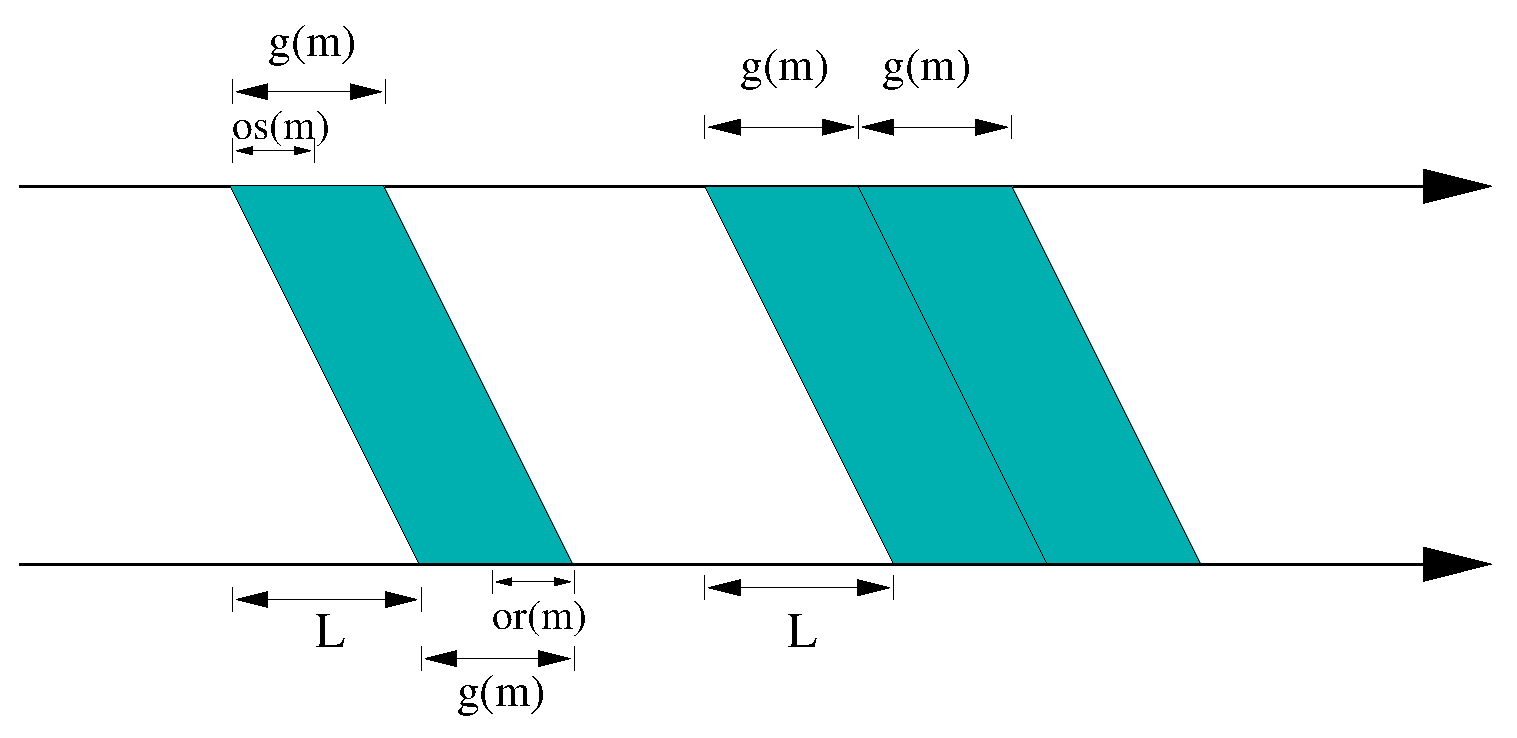
\includegraphics[width=0.7\linewidth]{images/p2p/plogp-struct}

\caption{\label{Figure: pLogP}Représentation d'une communication avec pLogP}

\end{figure}


En conséquence de cette nouvelle interprétation du \emph{gap}, les
paramètres $o_{s}$ et $o_{r}$ ont une importance moins évidente,
une fois que leur coût dans un réseau local est souvent recouvert
par celui du gap.  Ainsi, pour représenter le temps nécessaire à la transmission d'un
message de taille \emph{m} entre deux noeuds avec des primitives de
communication bloquante, le modèle pLogP utilise l'expression $L+g(m)$,
au lieu de $L+g+2o$ comme dans le modèle LogP. 


La variation des paramètres vis-à-vis de la taille des messages et des politiques d'émission est mise en évidence en Figure \ref{Figure: logp x hockney}, où on affiche les différents temps de communication mesurés avec la bibliothèque applicative LAM-MPI \cite{LAM04}. On observe un
changement de politique d'acquittement quand la taille des messages dépasse les 64 Ko, de manière à ce que le coût du gap dépend à la fois
de la saturation de la fenêtre TCP et de la politique d'acquittement.

%
\begin{figure}
\centering
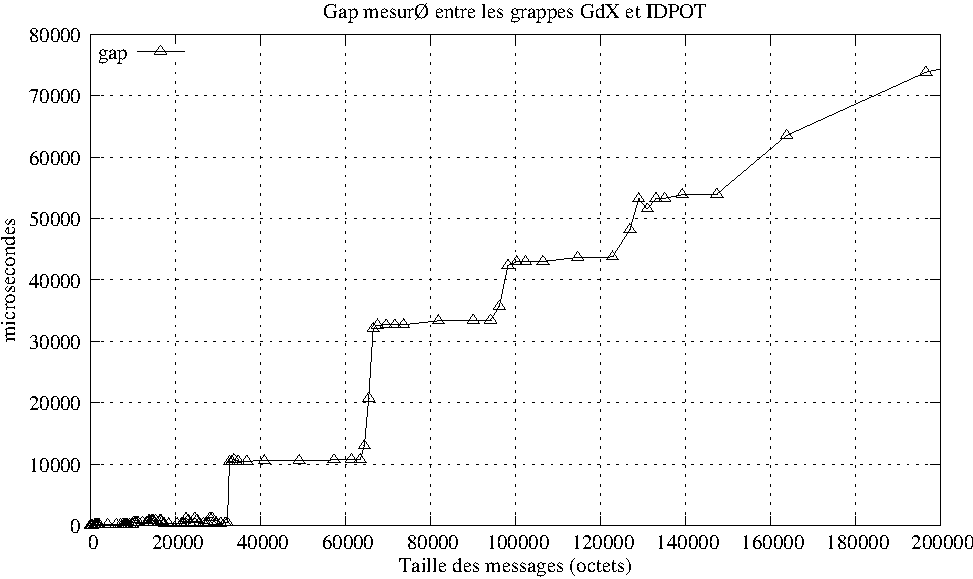
\includegraphics[width=0.7\linewidth]{images/p2p/hockney-logp1}

\caption{\label{Figure: logp x hockney}Valeurs de gap mesurés entre deux grappes
distantes (GdX et IDPOT)}

\end{figure}

\subsection{\label{sec:Broadcast}Exemple d'utilisation: modélisation d'un Broadcast\emph{: MPI\_Bcast}}

Une opération de \emph{Broadcast} s'effectue quand un seul processus,
appelé \emph{racine,} envoie le même message de taille \emph{m} à
tous les autres $(P-1)$ processus. 


L'approche classique pour implémenter l'opération \emph{Broadcast} utilise
des arbres qui sont décrits par deux paramètres, \emph{d} et \emph{h},
où \emph{d} est le nombre maximum de successeurs qu'un noeud peut
avoir, et \emph{h} est la hauteur de cet arbre, le chemin le plus
long qui relie la racine et les feuilles de cet arbre. Plus généralement,
des arbres de diffusion avec différents degrés \emph{d} et \emph{h}
peuvent être générés à partir d'un algorithme de type \emph{arbre-alpha}
(\emph{alpha-tree} en anglais) suggéré par Bernaschi et Ianello \cite{Bernaschi98}.
À l'aide de cet algorithme et des paramètres du réseau, un arbre optimal
peut être construit à partir des paramètres du réseau et avec \emph{d,
	h $\in$}{[}1...\emph{P}-1] tel que $\sum_{i=o}^{h}d^{i}\geq P$ soit
respecté. %Cependant, pour une question de simplicité, la plupart des
%implémentations MPI utilisent des formes fixes telles que les arbres
%plats ou les arbres binomiaux. 

La performance des différentes formes fixes dépend surtout des paramètres
du réseau, notamment le \emph{gap}, la latence et le nombre de noeuds.
Par conséquent, un réseau avec une latence faible par rapport au \emph{gap}
favorise les algorithmes de type Arbre Binaire et Arbre Binomial,
qui cherchent à minimiser le temps de communication par la multiplication
des sources de transmission. Au contraire, si la latence est trop
élevée par rapport au \emph{gap}, les algorithmes de type Arbre Plat
sont favorisés, où un seul processus envoie des messages à tous les
autres. 

%De ce fait, la plupart des implémentations MPI utilisent deux formes
%fixes, un Arbre Plat pour un nombre réduit de noeuds (jusqu'à 3 noeuds),
%et un Arbre Binomial pour un plus grand nombre de noeuds. Cela est
%dû au fait que généralement les arbres Binomiaux sont optimaux pour
%les réseaux homogènes locaux (dont une faible latence) ; l'utilisation
%des arbres Plats ne se fait que pour un nombre très réduit de processus,
%et cela seulement pour minimiser le coût de construction de l'arbre
%de diffusion.

À la diversité de formes fixes s'ajoutent aussi différentes techniques
d'implémentation. En effet, certaines techniques peuvent s'appliquer
à des situations spécifiques, comme par exemple, l'envoi de messages
avec des tailles plus importantes ; dans ce cas, un message de \emph{rendez-vous} est
envoyé préalablement pour préparer le récepteur, réduisant ainsi le
stockage des messages dans des buffers temporaires. Autre technique
souvent employée est l'utilisation des primitives de communication
non bloquantes pour permettre le recouvrement des communications et
du calcul. Il faut néanmoins compter que ces techniques apportent
un coût supplémentaire aux opérations : alors que le \emph{rendez-vous}
ajoute une étape de communication de plus, la communication non bloquante
est obtenue à partir de la copie des données vers des buffers intermédiaires.
Dans le premier cas le surcoût est constant et correspond à l'envoi
de deux messages de taille zéro, tandis que le deuxième cas a un coût
qui dépend de la taille du message, et qui correspond à $o_{s}$.

À partir des modèles de coût LogP \cite{Culler96} et pLogP \cite{Kielmann01}
et de travaux comme ceux de Huse \cite{Huse99}, Vadhiyar \cite{Vadhiyar00}
et autres, nous avons déduit les formules qui représentent différentes
stratégies de communication évaluées dans ce travail, comme indiqué
dans le Tableau \ref{table:bcast_models_classique}. Certaines de
ces stratégies sont clairement inefficaces, comme par exemple le broadcast
en Chaîne, qui exécute $P-1$ communications en série. D'autres stratégies,
comme les variantes \emph{rendez-vous}, ne sont utilisées qu'à partir
d'une taille de message suffisamment grande, ce qui minimise l'impact
des étapes de communication supplémentaires dues au \emph{rendez-vous}.
%Ainsi, nous avons choisi les stratégies d'Arbre Plat et d'Arbre Binomial
%pour représenter les algorithmes classiques, après avoir vérifié que
%ceux-ci sont les deux stratégies utilisées par défaut dans l'implémentation
%LAM-MPI \cite{LAM04}. Ces stratégies seront analysées dans la section
%\ref{sub:Broadcast_Practical}, où les modèles de communication seront
%validés à travers des résultats issus des expérimentations pratiques.

%
\begin{table}[h]
	\centering
		\begin{tabular}{|c|c|}
			\hline 
			\textbf{\small Stratégie} & \textbf{\small Modèle de Communication}\tabularnewline
			\hline
			\hline 
			{\small Arbre Plat} & {\small $L+(P-1)\times g(m)$}\tabularnewline
			\hline 
			{\small Arbre Plat Rendez-vous} & {\small $3\times L+(P-1)\times g(m)+2\times g(1)$}\tabularnewline
			\hline 
			{\small Chaîne} & {\small $(P-1)\times(g(m)+L)$}\tabularnewline
			\hline 
			{\small Chaîne Rendez-vous} & {\small $(P-1)\times(g(m)+2\times g(1)+3\ \times L)$}\tabularnewline
			\hline 
			{\small Arbre Binaire} & {\small $\leq\lceil log_{2}P\rceil\times(2\times g(m)+L)$}\tabularnewline
			\hline 
			{\small Arbre Binomial} & {\small $\lceil log_{2}P\rceil\times L+\lfloor log_{2}P\rfloor\times g(m)$}\tabularnewline
			\hline 
			{\small Arbre Binomial Rendez-vous} & {\small $\lceil log_{2}P\rceil\times(2\times g(1)+3\times L)+\lfloor log_{2}P\rfloor\times g(m)$}\tabularnewline
			\hline
		\end{tabular}
		
	
	\caption{\label{table:bcast_models_classique}Modèles de communication pour
		le \emph{Broadcast}}
	
\end{table}

%\subsubsection{\label{sub: approches par segmentation}Approches par segmentation}

Une autre possibilité de construire un \emph{Broadcast} est la composition
des chaînes de retransmission \cite{Barnett96}. Cette stratégie,
possible grâce à la segmentation des messages, présente des avantages
importants, comme l'indiquent \cite{Kielmann01}\cite{Thakur03}\cite{Beaumont04a}.
Dans un \emph{Broadcast} Segmentée, la transmission des messages en
segments permet le recouvrement de la transmission d'un segment \emph{k}
et la réception du segment \emph{k}+1, minimisant le \emph{gap}.

Dans ce cas, nous considérons que le segment de taille \emph{s} d'un
message \emph{m} est un multiple de la taille du type basique de données
qui est transmis, divisant alors le message initial \emph{m} en \emph{k}
segments. Par conséquent, \emph{g(s)} représente le \emph{gap} d'un
segment de taille \emph{s}. Toutefois, le choix de la taille des segments
reste dépendant des caractéristiques du réseau. En effet, l'utilisation
de segments trop petits a un surcoût non-négligeable dû à l'en-tête
du message, alors que l'utilisation des segments trop grands ne permet
pas l'exploitation intégrale du débit du réseau. 

La recherche de la taille de segment \emph{s} qui minimise le temps
de communication se fait à l'aide des modèles de communication présentés
dans le Tableau \ref{table:bcast_models_seg}. D'abord, on cherche
une taille de segment \emph{s} qui minimise le temps de communication
parmi $s=m/2^{i}\;\mathrm{pour}\; i\in[0\ldots log_{2}m]$. Ensuite,
on peut affiner la recherche de la taille optimale avec l'aide d'heuristiques
comme le \emph{\og local hill-climbing} \fg{} \cite{Kielmann01}.

%
\begin{table}[h]
	\centering
		\begin{tabular}{|c|c|}
			\hline 
			\textbf{\small Stratégie} & \textbf{\small Modèle de Communication}\tabularnewline
			\hline
			\hline 
			{\small Arbre Plat Segmenté} & {\small $L+(P-1)\times(g(s)\times k)$}\tabularnewline
			\hline 
			{\small Chaîne Segmentée (Pipeline)} & {\small $(P-1)\times(g(s)+L)+(g(s)\times(k-1))$}\tabularnewline
			\hline 
			{\small Arbre Binomial Segmenté} & {\small $\lceil log_{2}P\rceil\times L+\lfloor log_{2}P\rfloor\times g(s)\times k$}\tabularnewline
			\hline
			{\small Pieuvre avec un degré }\emph{\small d} & {\small $(d+\lceil\frac{P-(2^{d}+1)}{(2^{d}+1)}\rceil)\times(g(s)+L)+(g(s)\times(k-1))$}\tabularnewline
			\hline
			{\small Scatter/Collection \cite{Thakur03}} & {\small $(log_{2}P+P-1)\times L+2\times(\frac{p-1}{p})\times g(m)$}\tabularnewline
			\hline
		\end{tabular}
	
	\caption{\label{table:bcast_models_seg}Modèles de communication segmentée
		pour le \emph{Broadcast}}
	
\end{table}

%
%Dans les pages suivantes nous décrivons les stratégies qui utilisent
%la segmentation.
%
%
%\subsubsection*{Chaîne segmentée}
%
%La stratégie la plus simple de broadcast segmenté est la Chaîne Segmentée,
%appelée aussi \emph{pipeline}, présentée dans la Figure \ref{Figure: Chaine et segmentation}.
%La Chaîne Segmentée présente des performances assez avantageuses quand
%la taille des messages est considérablement grande, et surtout si
%la latence est réduite. Malgré ces performances, une implémentation
%en Chaîne Segmentée est sujette à certaines instabilités dues à la
%variation de performance des différents processus qui composent la
%chaîne. En effet, il suffit qu'un processus retarde la transmission
%des segments pour que l'exécution du broadcast soit perturbée. 
%
%%
%\begin{figure}[h]
%	\centering
%	\includegraphics[width=0.45\linewidth]{images/modeles/definitions/chainseg}
%	\caption{\label{Figure: Chaine et segmentation}Structure de communication
%		d'une Chaîne Segmentée}
%	
%\end{figure}
%
%
%
%\subsubsection*{Pieuvre}
%
%Si une chaîne est trop sensible à l'accumulation des retards des processus,
%une alternative suffisamment efficace est l'implémentation d'une stratégie
%hybride, qui mélange à la fois un Arbre Plat ou Binomial et des chaînes
%segmentées. Cette stratégie, appelée \emph{pieuvre} (ou \emph{k-chain}
%en anglais \cite{Pjesivac-Grbovic05}, Figure \ref{Figure: k-chain}) utilise
%un petit \og coeur \fg{} en forme d'arbre plat ou binomial, dont
%les processus donnent à leur tour naissance à plusieurs chaînes. 
%
%%
%\begin{figure}[h]
%	\centering
%		\includegraphics[width=0.25\linewidth]{images/modeles/definitions/bcastkchain}
%		
%	\caption{\label{Figure: k-chain}Structure de fonctionnement d'un arbre \emph{pieuvre}}
%	
%\end{figure}
%
%
%En conséquence, les chaînes formées sont plus courtes et plus nombreuses
%; les effets dus au retard d'un processus affectent seulement un groupe
%de processus, et le retard accumulé sera moins répandu dans les chaînes
%de diffusion. Ceci dit, un désavantage de cette stratégie par rapport
%à la Chaîne Segmentée classique est que le nombre de processus doit
%être suffisamment grand pour que l'accumulation des latences compense
%le coût initial des arbres de diffusion. Dans les expériences effectuées
%dans le cadre de ce travail, la performance de la pieuvre n'a pas
%pu dépasser celle de la chaîne segmentée, malgré un léger gain de
%performance par rapport à l'arbre binomial. Pour cette raison, et
%à cause de sa complexité, nous avons préféré l'étude de la chaîne
%segmentée, technique déjà utilisée pour la distribution de données
%à large échelle. 
%
%
%%\subsubsection*{Scatter/Collection}
%%
%%L'algorithme en arbre binomial est adéquat aux petits messages à cause
%%de son coût de latence logarithmique, tandis qu'un algorithme de type
%%Chaîne Segmentée peut s'avérer efficace pour les grands messages.
%%Cependant, l'algorithme en Chaîne Segmentée requiert une performance
%%uniforme de tous les processus, sinon sa performance est trop sujette
%%à des variations. 
%%
%%Une alternative plus sûre pour la diffusion de grands messages est
%%l'algorithme Scatter-Collection, proposé par Van de Geijn et \emph{al.}
%%\cite{Barnett96}. Dans cet algorithme, le message est d'abord partagé
%%entre les processus à l'aide d'une opération similaire à MPI\_Scatter
%%; ensuite, les données sont regroupées avec une opération similaire
%%à MPI\_Allgather. Le temps d'exécution est alors la somme du temps
%%d'exécution du \emph{Scatter} et du \emph{Allgather}. 
%%
%%En effet, Thakur \emph{et al.} \cite{Thakur03} utilisent cette technique
%%pour l'implémentation de MPI\_Bcast adaptée aux grands messages, où
%%un algorithme binomial est utilisé pour le \emph{Scatter} et un algorithme
%%en anneau pour le \emph{Allgather}.
%%
%%
%\subsubsection*{Segmentation et arbres de diffusion}
%
%Si dans certains cas la segmentation peut augmenter la performance
%de certaines stratégies de diffusion, cela ne s'applique pas à toutes
%les stratégies de communication. Par exemple, l'apport de l'utilisation
%conjointe de la segmentation de messages et des stratégies de broadcast
%en arbre Plat ou Binomial dépend surtout des paramètres de communication
%(\emph{L} et \emph{g}), une fois que ces stratégies obligent une interdépendance
%entre processus par rapport à la distribution des données. Pour mieux
%illustrer cette situation, la Figure \ref{Figure: Arbre Binomial et Segmentation}
%représentent le schéma de communication pour l'algorithme en arbre
%binomial avec $L=1$ et $g=1$. Nous observons que la structure de
%cet algorithme oblige un flux de données qui n'est pas adapté à l'enchaînement
%des communications, comme c'était le cas avec la chaîne segmentée
%\ref{Figure: Chaine et segmentation}. 
%
%
%
%\begin{figure}[t]
%	\centering
%		\includegraphics[width=0.45\linewidth]{images/modeles/definitions/binomialtrad} \includegraphics[width=0.45\linewidth]{images/modeles/definitions/binomialseg}
%	\caption{\label{Figure: Arbre Binomial et Segmentation}La stratégie en Arbre
%		Binomial sans et avec segmentation avec L=1 et g=1}
%	
%\end{figure}
%
%
%En effet, pour des valeurs de $g\geq L$, la chaîne segmentée est
%la forme optimale; seulement si $g\leq L$ les autres formes d'arbre
%deviennent plus intéressantes, car elles rendent possible le recouvrement
%de la latence de communication par des émissions successives.


\subsection{\label{sub:Broadcast_Practical}Validation des modèles}

Pour valider ces modèles de communication, nous avons choisi la comparaison
entre les prédictions des modèles et les résultats réels obtenus à
partir d'expérimentations sur différentes plates-formes réseaux. Pour
illustrer notre approche, nous avons comparé des implémentations de
MPI\_Bcast selon les stratégies Arbre Plat, Arbre Binomial et Chaîne
Segmentée. 
%Dans les prochaines pages nous présentons l'analyse des
%expérimentations effectuées sur chaque plate-forme réseau différente. 


\subsubsection*{Réseau Fast Ethernet}

Comme nous pouvons observer dans les Figures \ref{Figure:Comparison-Bcast_Flat_FEth},
\ref{Figure:Comparison-Bcast_Bin_FEth} et \ref{Figure:Comparison-Bcast-Chain_FEth},
les prédictions des trois stratégies d'implémentation représentent presque
fidèlement les résultats expérimentaux obtenus sur un cluster.
%le réseau Fast Ethernet. 

Plus spécifiquement, des différences entre les prédictions et les
valeurs réelles sont observées surtout dans le cas de la stratégie
en Arbre Binomial, où le temps mesuré pour l'envoi de petits messages
est plus élevé que celui prévu, et ne suit pas un comportement linéaire
par rapport à la taille des messages. Cette variation de performance,
observée aussi dans des expériences avec d'autres réseaux,
%le réseau Giga Ethernet,
a été l'objet d'analyses précédentes (cette discussion peut être retrouvée
dans les articles \cite{Steffenel04a} et \cite{Steffenel04c}) et dont l'origine des retards
est due à l'implémentation des politiques d'acquittement TCP sur Linux, qui retarde
des messages même si l'option \emph{socket} TCP\_NODELAY est activée. 

En effet, parfois un seul message
à chaque \emph{n} messages transmis n'est pas acquitté comme il le
faut. Cette défaillance du protocole d'acquittement induit un temps supplémentaire
nécessaire à la retransmission du message et à son acquittement.  

%
\begin{figure}[h]
	\centering
		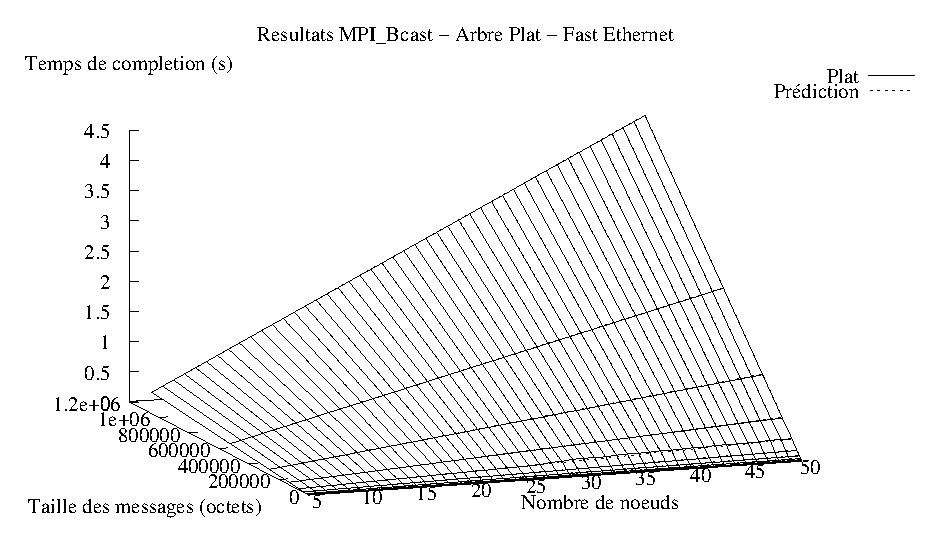
\includegraphics[width=0.6\linewidth]{images/modeles/FEth/Bcast/comp_Flat}
		
	\caption{\label{Figure:Comparison-Bcast_Flat_FEth}Les performances réelles
		et prédites pour l'Arbre Plat avec un réseau Fast Ethernet}
	
\end{figure}


%
\begin{figure}[h]
	\centering
		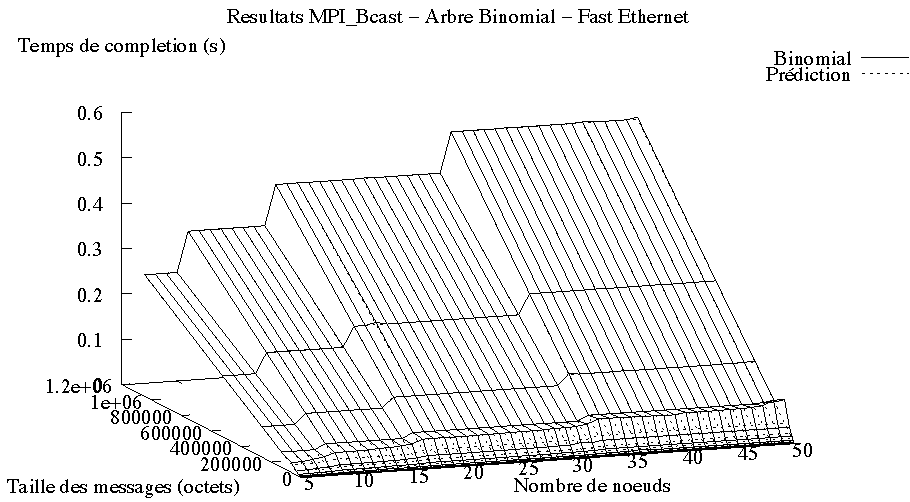
\includegraphics[width=0.6\linewidth]{images/modeles/FEth/Bcast/comp_Binomial}
	
	\caption{\label{Figure:Comparison-Bcast_Bin_FEth}Les performances réelles
		et prédites pour l'Arbre Binomial avec un réseau Fast Ethernet}
	
\end{figure}


%
\begin{figure}[h]
	\centering
		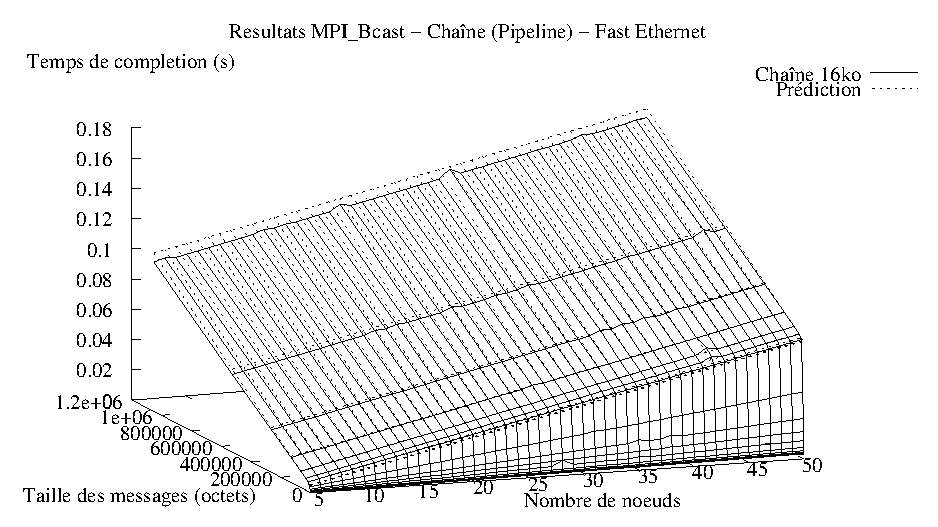
\includegraphics[width=0.6\linewidth]{images/modeles/FEth/Bcast/comp_Chain_16384}
	
	\caption{\label{Figure:Comparison-Bcast-Chain_FEth}Les performances réelles
		et prédites pour la Chaîne Segmentée avec un réseau Fast Ethernet}
	
\end{figure}

%
%Nous pouvons également observer dans la Figure \ref{Figure:Comparison-between-models Bcast FEth}
%le comportement des trois stratégies et leurs prédictions lorsque
%varie le nombre de processus. Nous observons que la stratégie en Arbre
%Plat est beaucoup moins performante que les deux autres stratégies,
%et sa performance décroît avec l'augmentation du nombre de processus
%communicants, alors que les autres stratégies sont beaucoup plus stables
%par rapport au nombre de processus. Cela est du au modèle de communication
%employé par la stratégie en Arbre Plat, qui la rend directement dépendante
%du nombre de processus et du surcoût d'envoi des messages (\emph{gap}).
%Les stratégies en Arbre Binomial et en Chaîne Segmentée sont moins
%sensibles à l'augmentation du nombre de processus car la première
%stratégie a un coût logarithmique, alors que la deuxième est linéairement
%dépendante de la latence, qui a une valeur bien plus réduite. 
%
%%
%\begin{figure}[h]
%	\centering
%		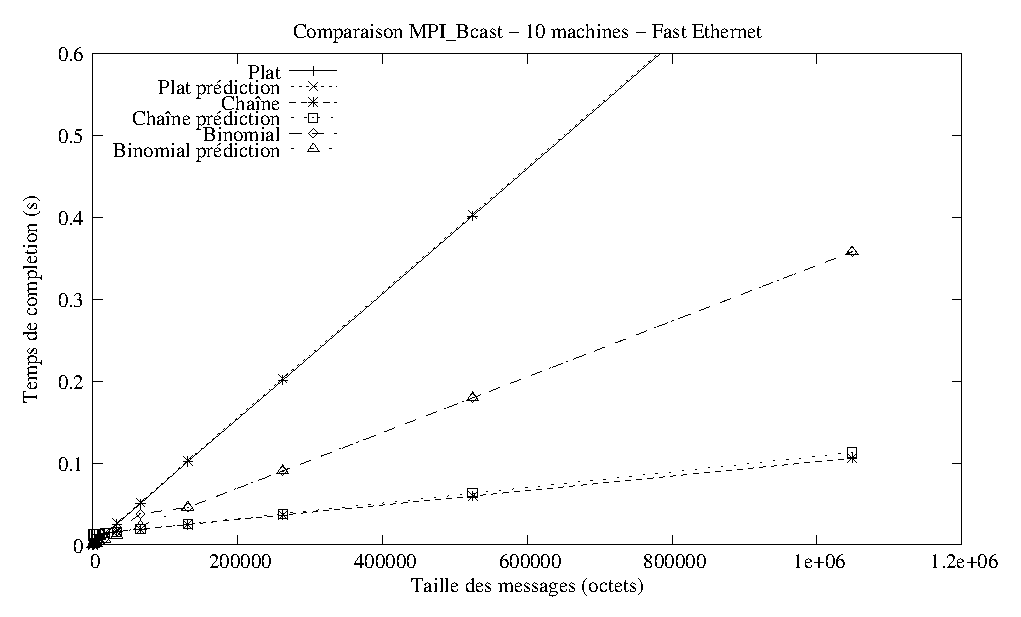
\includegraphics[width=0.6\linewidth]{images/modeles/FEth/Bcast/comp10}
%		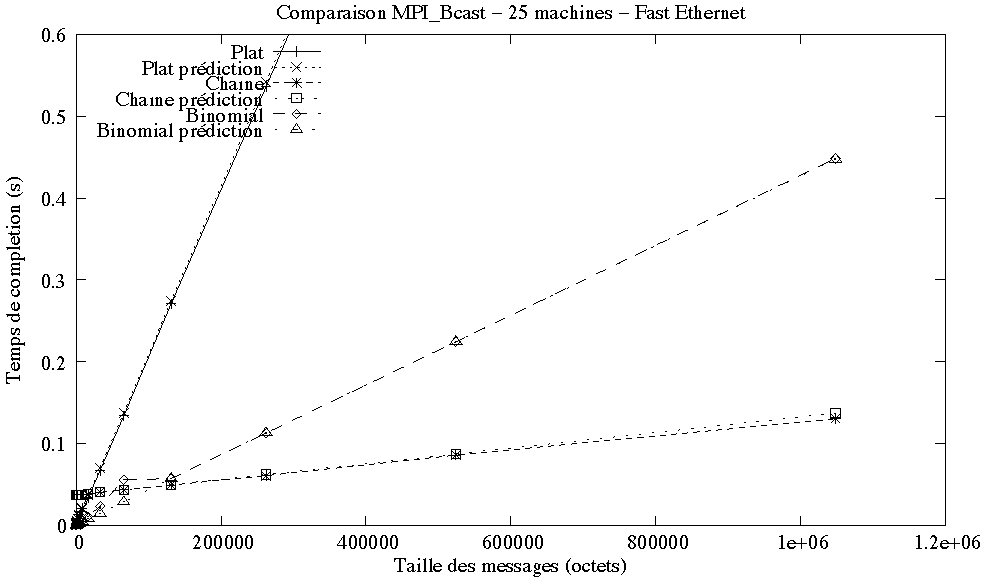
\includegraphics[width=0.6\linewidth]{images/modeles/FEth/Bcast/comp25}
%		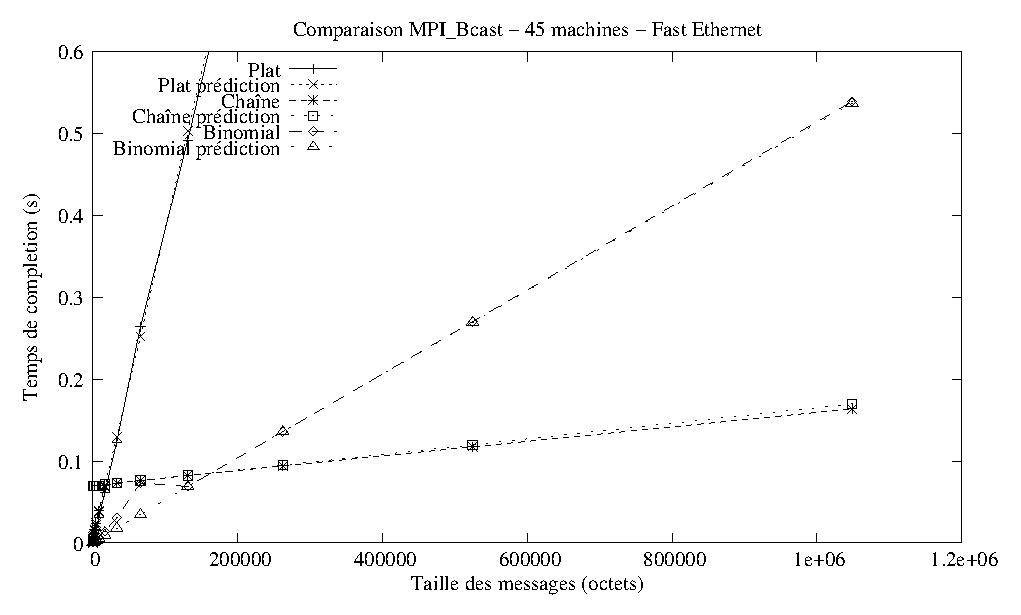
\includegraphics[width=0.6\linewidth]{images/modeles/FEth/Bcast/comp45}
%	
%	\caption{\label{Figure:Comparison-between-models Bcast FEth}Comparaison entre
%		les résultats réels et prédits pour des groupes de 10, 25 et 45 machines
%		dans un réseau Fast Ethernet}
%	
%\end{figure}


Les variations de performance observées dans le cas de la stratégie
en Arbre Binomial sont plus visibles dans la Figure \ref{Figure:Erreur-Bcast-FEth}.
Ici, nous observons que les résultats réels, normalement très proches
des prédictions (à une marge de 10\% maximum), s'écartent des prédictions
jusqu'à 90\% pour des messages autour de 128 Ko. Néanmoins, ces variations
affectent des communications où la différence absolue n'est que de
quelques millisecondes, ce qui n'empêche pas l'utilisation des modèles
de communication pour choisir la meilleure stratégie de communication. 

%
\begin{figure}[h]
	\centering
			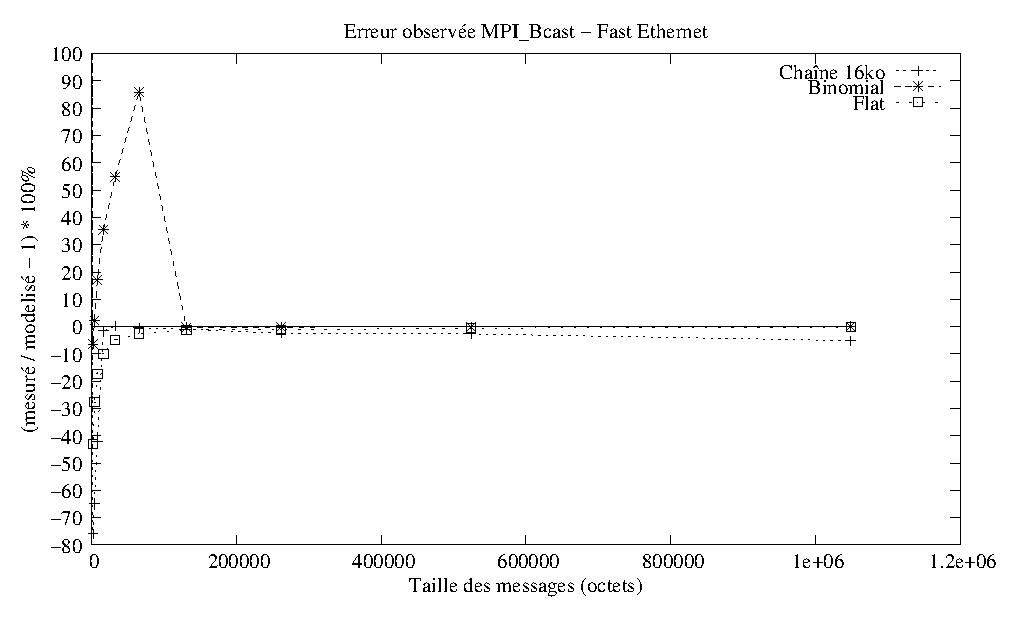
\includegraphics[width=0.6\linewidth]{images/modeles/FEth/Bcast/error}
		
	
	\caption{\label{Figure:Erreur-Bcast-FEth}L'erreur des prédictions par rapport
		aux valeurs mesurées, dans un réseau Fast Ethernet}
	
\end{figure}



%\subsubsection*{Réseau Giga Ethernet}
%
%Les résultats des expérimentations effectuées sur le réseau Giga Ethernet
%de la grappe \emph{Grid eXplorer} sont présentés dans les Figures
%\ref{Figure:Comparison-Bcast_Flat_GEth}, \ref{Figure:Comparison-Bcast_Bin_GEth}
%et \ref{Figure:Comparison-Bcast-Chain_GEth}. Si les prédictions pour
%la stratégie en Arbre Plat suivent fidèlement les résultats pratiques,
%nous observons des variations importantes dans les cas des stratégies
%en Arbre Binomial et en Chaîne Segmentée. Dans les deux cas, le temps
%des communications a subi une forte augmentation quand l'application
%utilise plus de 24 processus. Si l'origine de cette augmentation nécessite
%une investigation plus approfondie, nous considérons fortement la
%possibilité d'une surcharge du commutateur. En effet, la stratégie
%en Arbre Plat limite les communications à la capacité d'envoi du processus
%\emph{racine}, alors que les autres stratégies favorisent l'envoi
%simultané de messages par différents processus, ce qui peut surcharger
%le commutateur.
%
%%
%\begin{figure}[h]
%	\centering
%		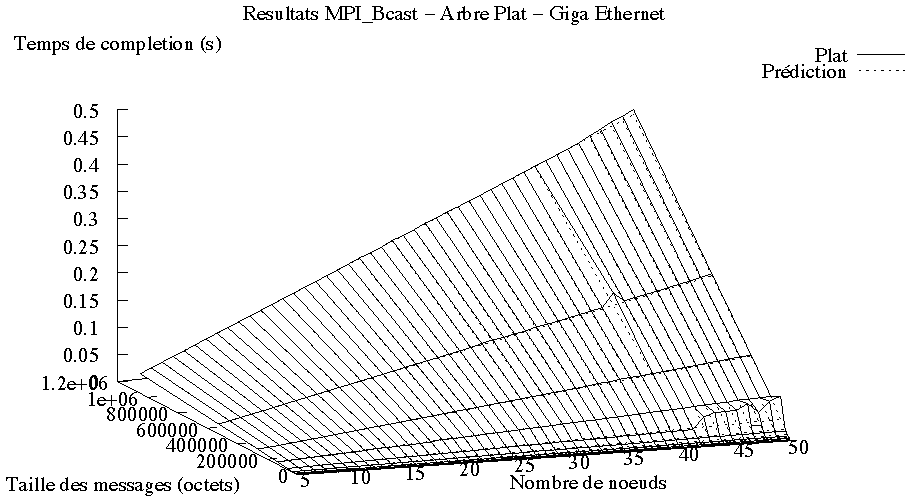
\includegraphics[width=0.6\linewidth]{images/modeles/GEth/Bcast/comp_Flat}
%	\caption{\label{Figure:Comparison-Bcast_Flat_GEth}Les performances réelles
%		et prédites pour l'Arbre Plat avec un réseau Giga Ethernet}
%	
%\end{figure}
%%
%\begin{figure}[h]
%	\centering
%		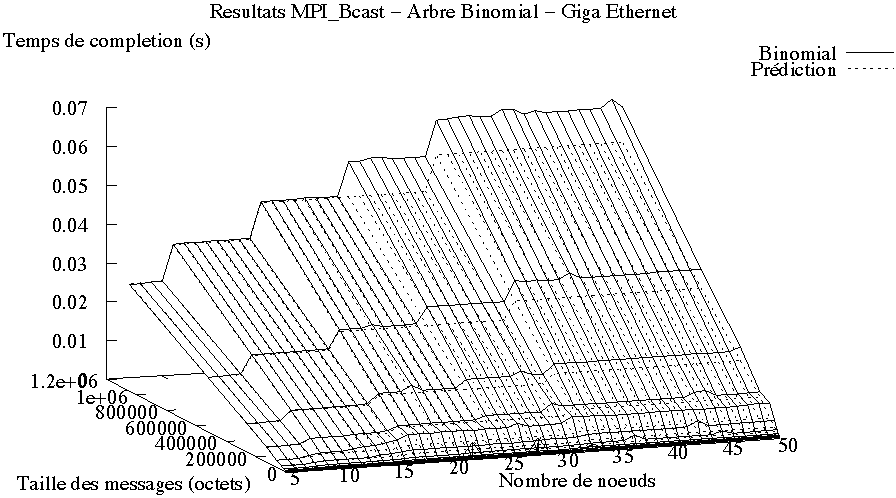
\includegraphics[width=0.6\linewidth]{images/modeles/GEth/Bcast/comp_Binomial}
%	
%	\caption{\label{Figure:Comparison-Bcast_Bin_GEth}Les performances réelles
%		et prédites pour l'Arbre Binomial avec un réseau Giga Ethernet}
%	
%\end{figure}
%
%
%%
%\begin{figure}[h]
%	\centering
%		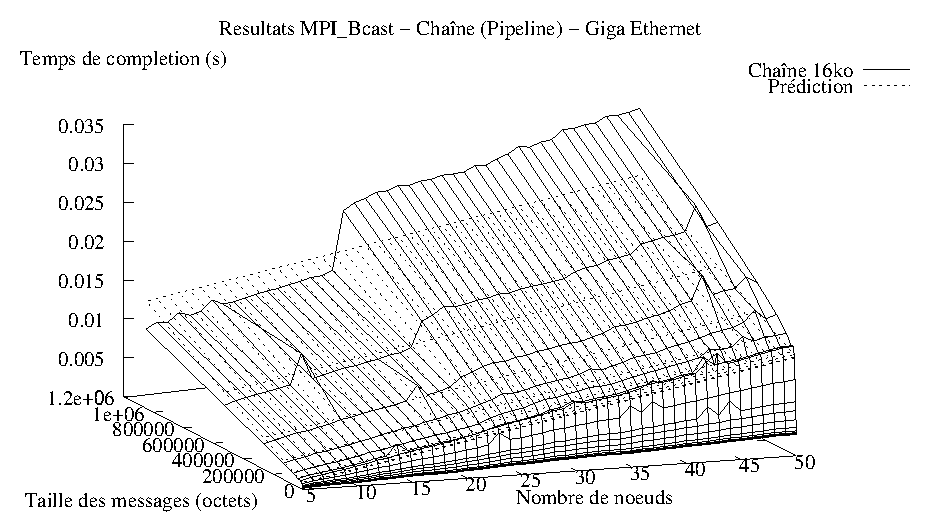
\includegraphics[width=0.6\linewidth]{images/modeles/GEth/Bcast/comp_Chain_16384}
%	
%	\caption{\label{Figure:Comparison-Bcast-Chain_GEth}Les performances réelles
%		et prédites pour la Chaîne Segmentée avec un réseau Giga Ethernet}
%	
%\end{figure}
%
%
%Toutefois, nous pouvons observer dans la Figure \ref{Figure:Comparison-between-models Bcast GEth}
%que si les prédictions ne correspondent pas exactement aux résultats
%réels, au moins elles suivent le comportement général des trois stratégies
%d'implémentation. Plus exactement, si nous considérons seulement le
%cas des 10 processus (et que par conséquent sont exemptés des effets
%dûs au commutateur), les prédictions sont très similaires aux résultats
%réels, comme atteste la Figure \ref{Figure:Comparison-between-models Bcast GEth}(a). 
%
%Dans tous les cas, nous observons que la stratégie en Arbre Plat est
%beaucoup moins performante que les deux autres stratégies, et que
%la Chaîne Segmentée présente la meilleure performance pour les grands
%messages (la meilleure stratégie pour l'envoi de petits messages dépend
%surtout du nombre de processus).
%
%%
%\begin{figure}[h]
%	\centering
%		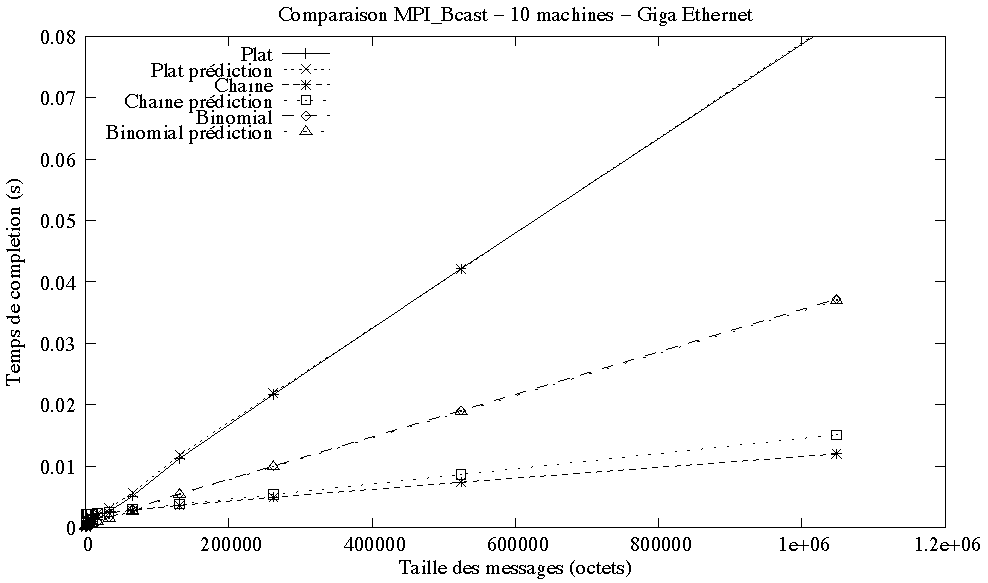
\includegraphics[width=0.6\linewidth]{images/modeles/GEth/Bcast/comp10}\\
%		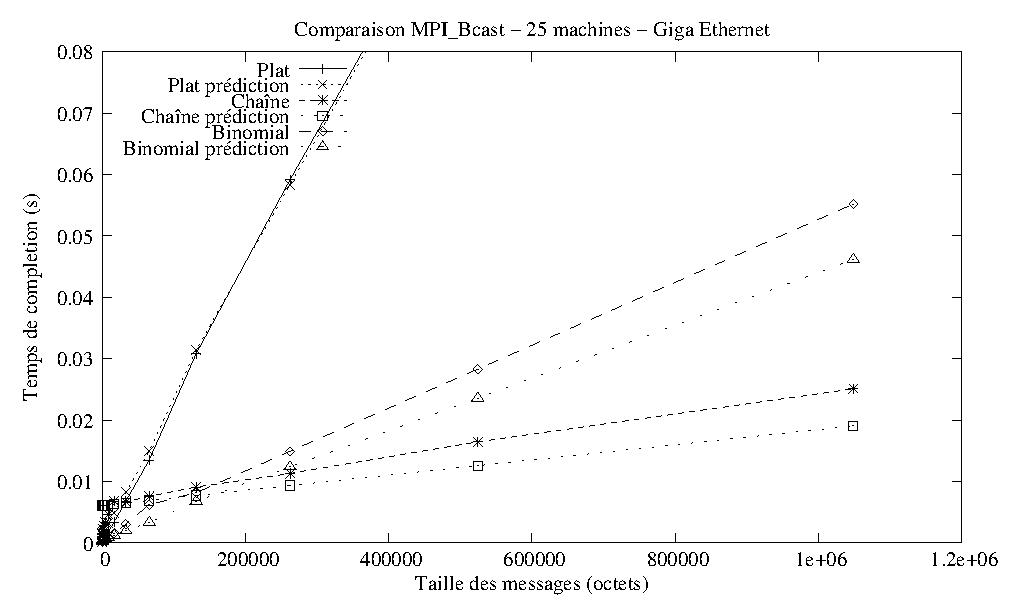
\includegraphics[width=0.6\linewidth]{images/modeles/GEth/Bcast/comp25}\\
%		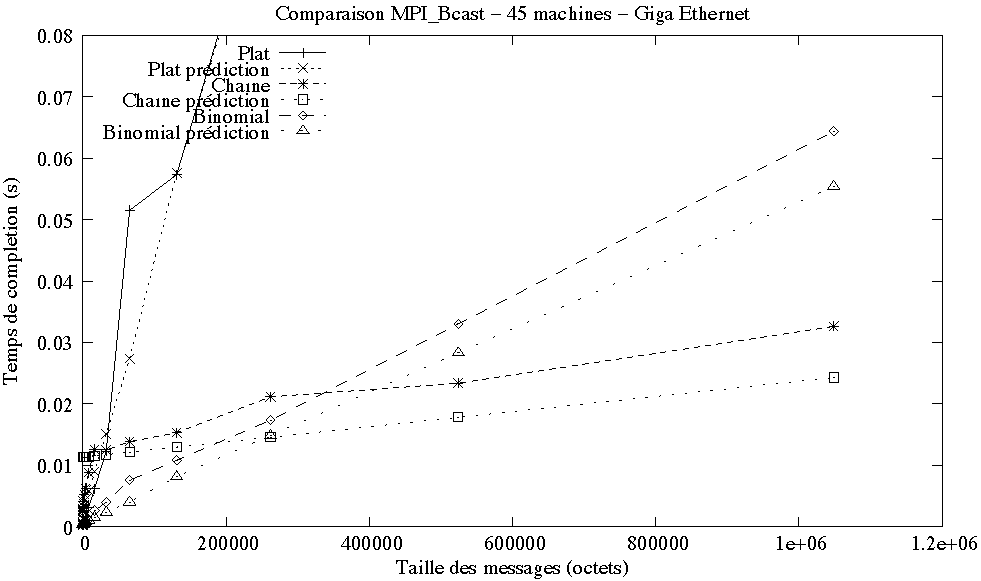
\includegraphics[width=0.6\linewidth]{images/modeles/GEth/Bcast/comp45}
%	\caption{\label{Figure:Comparison-between-models Bcast GEth}Comparaison entre
%		les résultats réels et prédits pour des groupes de 10, 25 et 45 machines
%		dans un réseau Giga Ethernet}
%	
%\end{figure}
%
%
%Étant donné que le surcout dû à la surcharge du commutateur est un
%facteur difficile à prédire, nous avons concentré l'analyse de l'erreur
%relative des prédictions au groupe de processus qui n'étaient pas
%sous l'influence du commutateur surchargé. Ainsi, nous pouvons observer
%dans la Figure \ref{Figure:Erreur_Bcast_GEth} que les prédictions
%sont suffisamment proches des résultats expérimentaux, avec une erreur
%généralement inférieure à 10\%. Nous pouvons aussi constater que l'approche
%en Arbre Binomial subit les mêmes variations déjà observées dans le
%cas du réseau Fast Ethernet avec des petits messages, ce qui corrobore
%l'hypothèse que l'implémentation du protocole TCP sous Linux occasionne
%arbitrairement des retards importants pour certains messages.
%
%%
%\begin{figure}[h]
%	\begin{centering}
%		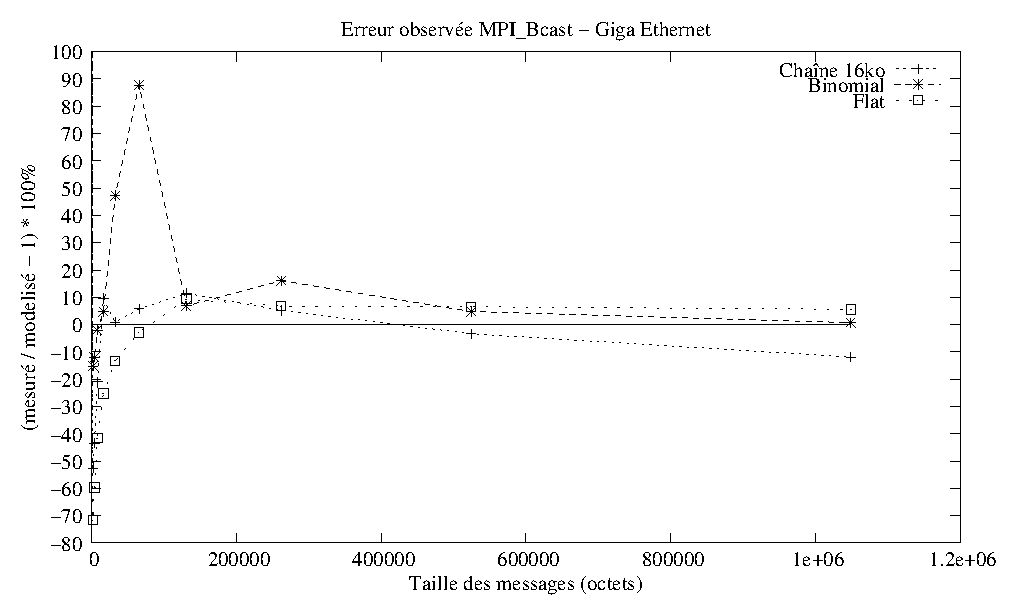
\includegraphics[width=0.6\linewidth]{images/modeles/GEth/Bcast/error}
%	\end{centering}
%	
%	\caption{\label{Figure:Erreur_Bcast_GEth}L'erreur des prédictions par rapport
%		aux valeurs mesurées, dans un réseau Giga Ethernet}
%	
%\end{figure}
%
%
%
%%\subsubsection*{Réseau Myrinet}
%%
%%
%%Les expériences conduites sur le réseau Myrinet de la grappe \emph{icluster-2}
%%sont présentées dans les Figures \ref{Figure:Comparison-Bcast_Flat_Myri},
%%\ref{Figure:Comparison-Bcast_Bin_Myri} et \ref{Figure:Comparison-Bcast-Chain_Myri}.
%%Similairement à ce qui a déjà été observé pour les réseaux Fast Ethernet
%%et Giga Ethernet, les modèles de communication des stratégies en Arbre
%%Plat et Arbre Binomial reproduisent fidèlement le comportement des
%%expériences pratiques. 
%%
%%%
%%\begin{figure}[h]
%%	\begin{centering}
%%		\begin{tabular}{c}
%%			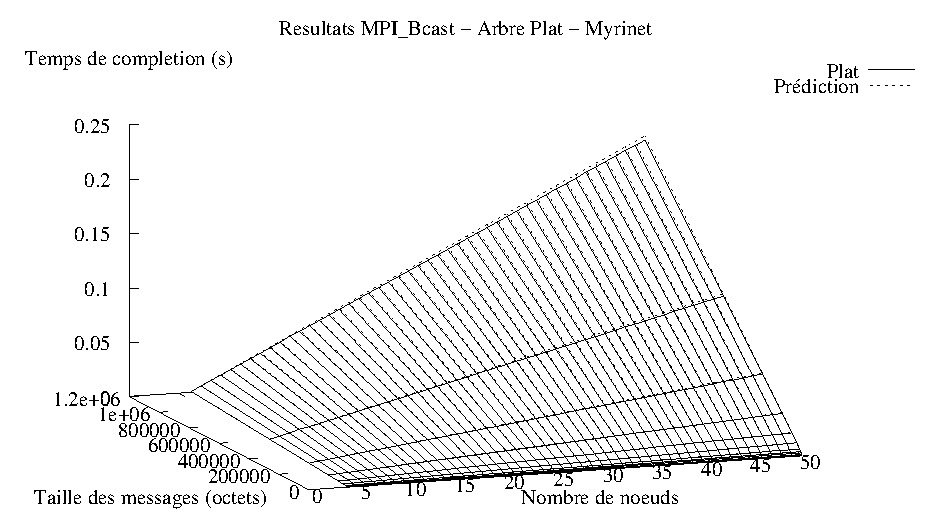
\includegraphics[width=0.6\linewidth]{images/modeles/Myrinet/Bcast/comp_Flat}\tabularnewline
%%		\end{tabular}\vspace{-0.5cm}
%%		\par\end{centering}
%%	
%%	\caption{\label{Figure:Comparison-Bcast_Flat_Myri}Les performances réelles
%%		et prédites pour l'Arbre Plat avec un réseau Myrinet}
%%	
%%\end{figure}
%%
%%
%%%
%%\begin{figure}[h]
%%	\begin{centering}
%%		\begin{tabular}{c}
%%			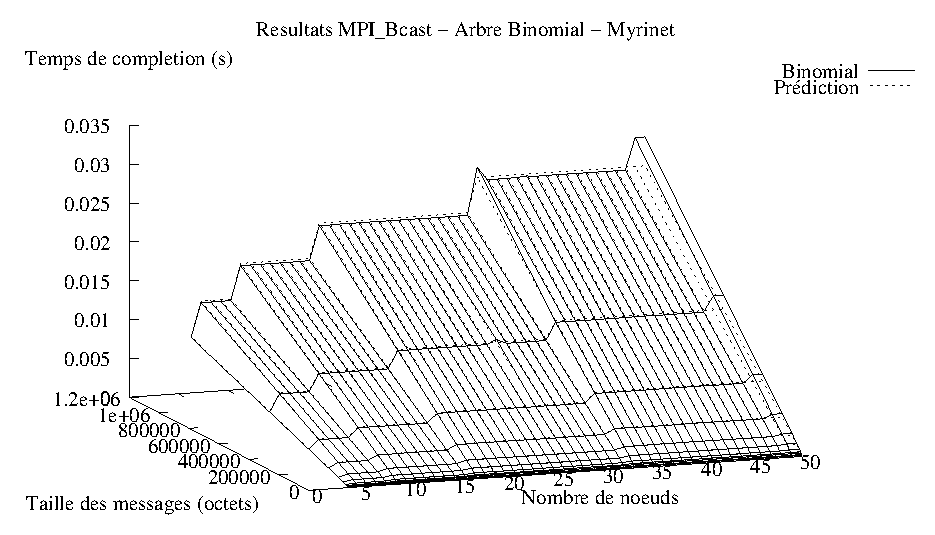
\includegraphics[width=0.6\linewidth]{images/modeles/Myrinet/Bcast/comp_Binomial}\tabularnewline
%%		\end{tabular}\vspace{-0.5cm}
%%		\par\end{centering}
%%	
%%	\caption{\label{Figure:Comparison-Bcast_Bin_Myri}Les performances réelles
%%		et prédites pour l'Arbre Binomial avec un réseau Myrinet}
%%	
%%\end{figure}
%%
%%
%%%
%%\begin{figure}[h]
%%	\begin{centering}
%%		\begin{tabular}{c}
%%			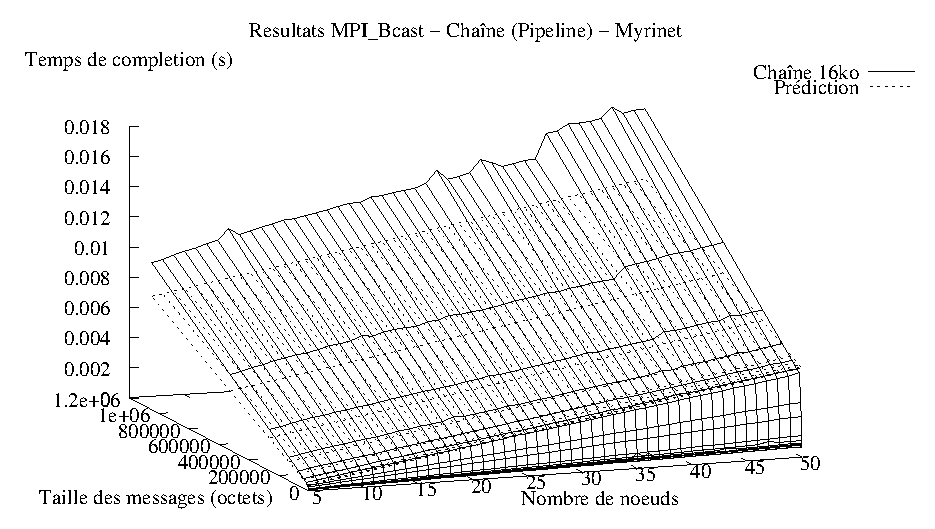
\includegraphics[width=0.6\linewidth]{images/modeles/Myrinet/Bcast/comp_Chain_16384}\tabularnewline
%%		\end{tabular}\vspace{-0.5cm}
%%		\par\end{centering}
%%	
%%	\caption{\label{Figure:Comparison-Bcast-Chain_Myri}Les performances réelles
%%		et prédites pour la Chaîne Segmentée avec un réseau Myrinet}
%%	
%%\end{figure}
%%
%%
%%Dans le cas de la Chaîne Segmentée toutefois les prédictions sous-estiment
%%le temps nécessaire à l'exécution du broadcast. Nous croyons que l'erreur
%%observée est liée au coût de la manipulation des segments. Ce coût,
%%qui normalement représente une petite partie du temps total d'exécution,
%%devient plus important quand l'environnement réseau utilisé est suffisamment
%%rapide, à l'exemple du réseau Myrinet, où la latence et le \emph{gap}
%%sont très faibles par rapport aux autres architectures réseau utilisées.
%%Pour vérifier si cette erreur est réellement due à la manipulation
%%des segments et pas au mauvais choix du segment, nous avons effectué
%%l'expérience avec d'autres tailles de segment, 32Ko et 64Ko (Figures
%%\ref{Figure:Comparison-Bcast-Chain_Myri_outrosseg}a et \ref{Figure:Comparison-Bcast-Chain_Myri_outrosseg}b).
%%Celles ci montrent d'un côté que le surcoût par rapport à la prédiction
%%reste importante, mais aussi que l'utilisation de segments plus grands
%%n'a pas permis la réduction du temps de communication.
%%
%%%
%%\begin{figure}[h]
%%	\begin{centering}
%%		\begin{tabular}{c}
%%			\subfigure[Chaîne segmentée avec 32Ko]{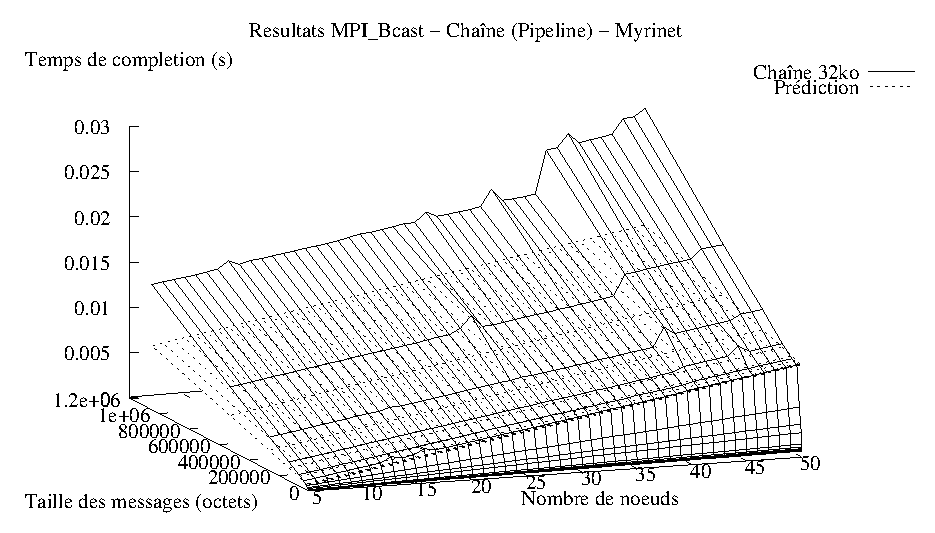
\includegraphics[width=0.6\linewidth]{images/modeles/Myrinet/Bcast/comp_Chain_32768}}\tabularnewline
%%		\end{tabular}\vspace{-0.5cm}\\
%%		\begin{tabular}{c}
%%			\subfigure[Chaîne segmentée avec 64Ko]{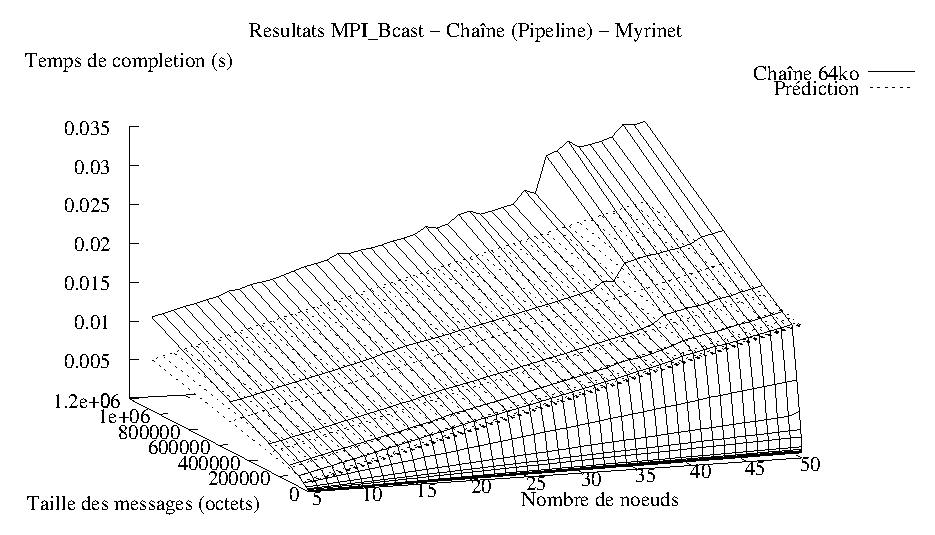
\includegraphics[width=0.6\linewidth]{images/modeles/Myrinet/Bcast/comp_Chain_65536}}\tabularnewline
%%		\end{tabular}\vspace{-0.5cm}
%%		\par\end{centering}
%%	
%%	\caption{\label{Figure:Comparison-Bcast-Chain_Myri_outrosseg}Les performances
%%		réelles et prédites pour la Chaîne Segmentée sur un réseau Myrinet
%%		avec différentes tailles de segment}
%%	
%%\end{figure}
%%
%%
%%Bien que les prédictions pour la Chaîne Segmentée ont une marge d'erreur
%%plus importante, nous pouvons observer dans la Figure \ref{Figure:Comparison-between-models Bcast Myri}
%%que les prédictions de cette stratégie sont encore suffisamment proches
%%pour permettre le choix de la meilleure stratégie à utiliser. Cependant,
%%avec le développement et la démocratisation d'architectures réseau
%%plus rapides, on peut envisager l'intégration de ce coût aux modèles
%%de communication, à l'exemple de l'approche proposée pour le patron
%%de communication \emph{Plusieurs vers Plusieurs Personnalisé}, décrite
%%dans la section \ref{sec:Alltoall}.
%%
%%%
%%\begin{figure}[h]
%%	\begin{centering}
%%		\vspace{-0.5cm}\begin{tabular}{c}
%%			\subfigure[10 machines]{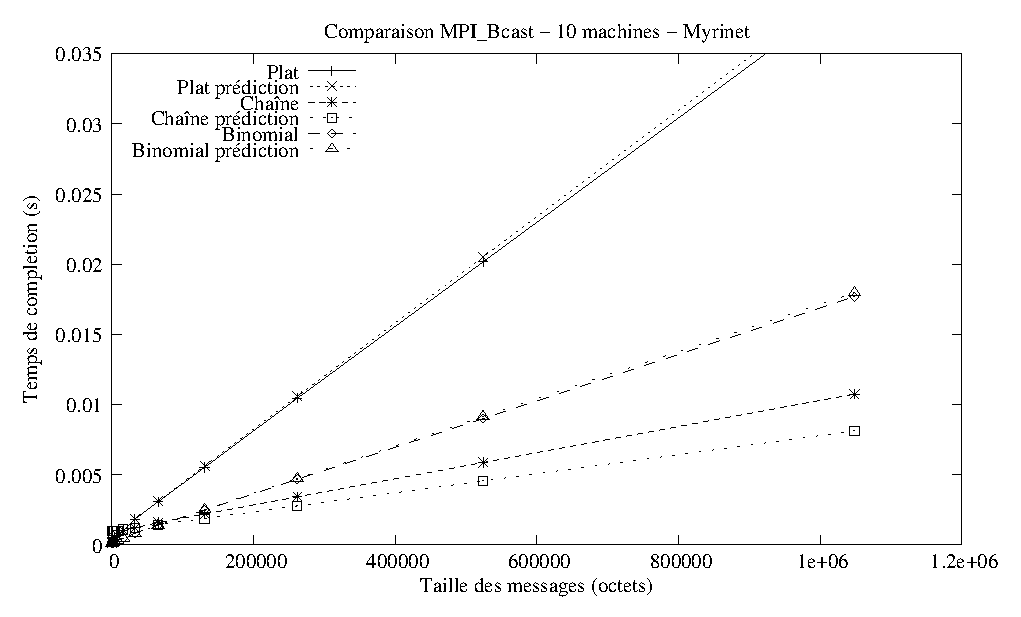
\includegraphics[width=0.6\linewidth]{images/modeles/Myrinet/Bcast/comp10}}\tabularnewline
%%		\end{tabular}\\
%%		\vspace{-0.5cm}
%%		\par\end{centering}
%%	
%%	\begin{centering}
%%		\begin{tabular}{c}
%%			\subfigure[25 machines]{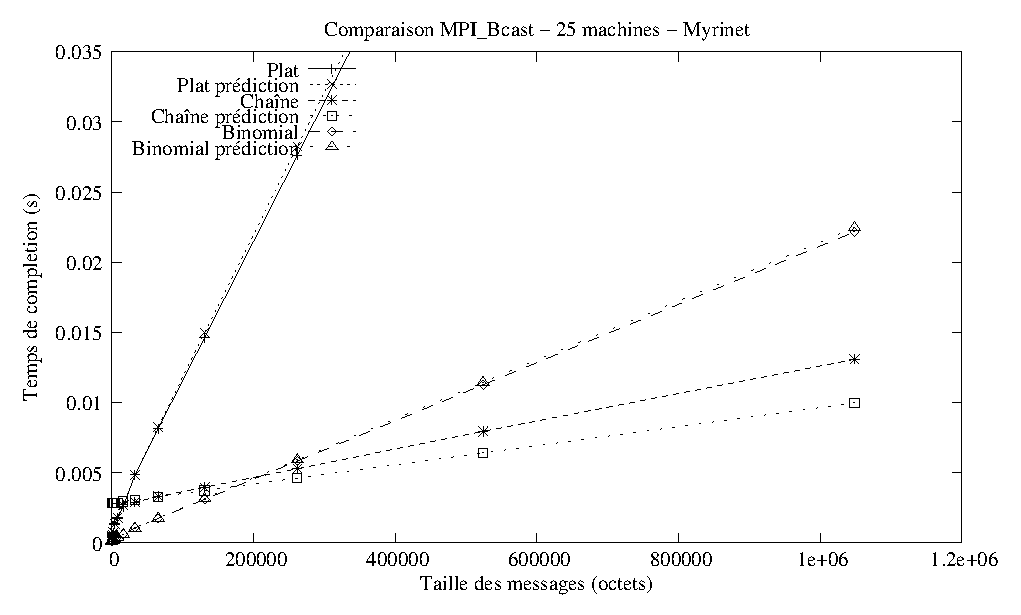
\includegraphics[width=0.6\linewidth]{images/modeles/Myrinet/Bcast/comp25}}\tabularnewline
%%		\end{tabular}\vspace{-0.5cm}
%%		\par\end{centering}
%%	
%%	\begin{centering}
%%		\begin{tabular}{c}
%%			\subfigure[45 machines]{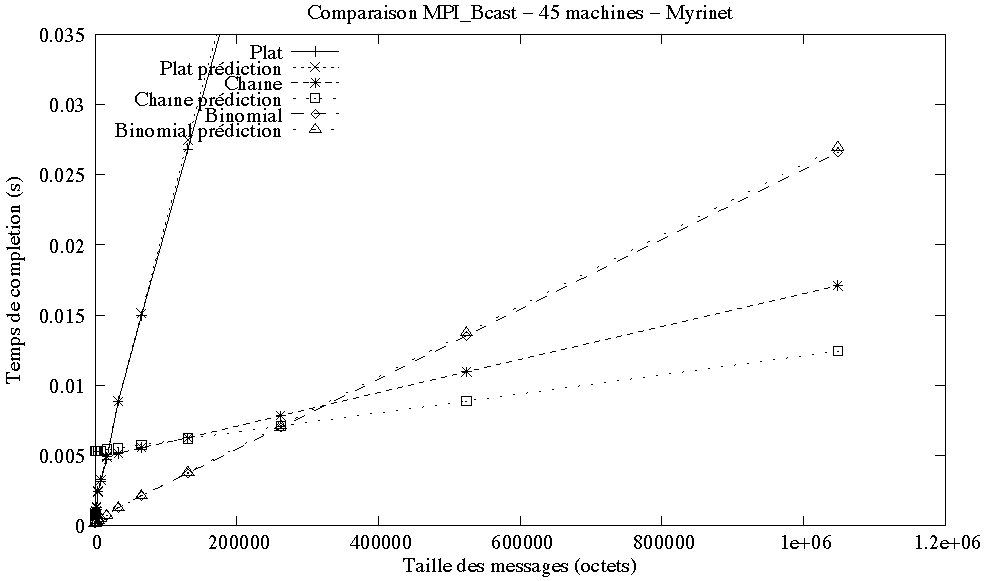
\includegraphics[width=0.6\linewidth]{images/modeles/Myrinet/Bcast/comp45}}\tabularnewline
%%		\end{tabular}\vspace{-0.5cm}
%%		\par\end{centering}
%%	
%%	\caption{\label{Figure:Comparison-between-models Bcast Myri}Comparaison entre
%%		les résultats réels et prédits pour des groupes de 10, 25 et 45 machines
%%		dans un réseau Myrinet}
%%	
%%\end{figure}
%%
%%
%%L'impact du coût dû à la segmentation des messages sur l'approche
%%Chaîne Segmentée peut être mieux observé à travers l'analyse de l'erreur
%%présentée dans la Figure \ref{Figure:Erreur Bcast Myri}. Alors que
%%les autres stratégies de communication ont une erreur insignifiante,
%%l'erreur des prédictions pour la Chaîne Segmentée peut dépasser les
%%30\% selon la taille de segment utilisée, mais se stabilise avec l'augmentation
%%de la taille des messages envoyés.
%%
%%%
%%\begin{figure}[h]
%%	\begin{centering}
%%		\begin{tabular}{c}
%%			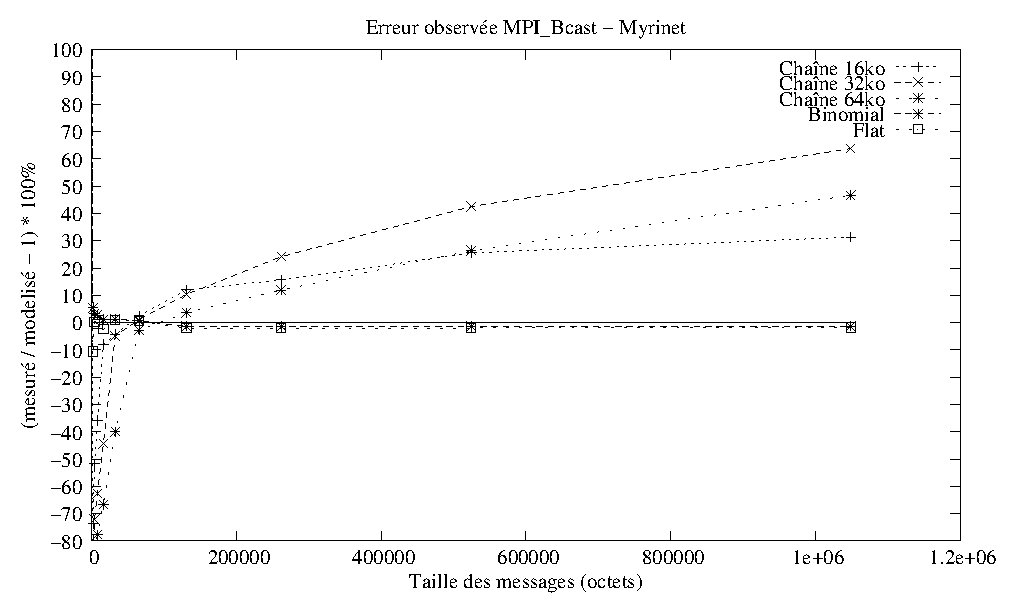
\includegraphics[width=0.6\linewidth]{images/modeles/Myrinet/Bcast/error}\tabularnewline
%%		\end{tabular}\vspace{-0.5cm}
%%		\par\end{centering}
%%	
%%	\caption{\label{Figure:Erreur Bcast Myri}L'erreur des prédictions par rapport
%%		aux valeurs mesurées, dans un réseau Myrinet}
%%	
%%\end{figure}
%%
%%
%%
%%
%%
%%
%%
%\section{Découverte de Topologie et Classification des Ressources \label{sec:reseaux-topo}}
%
%La connaissance de la topologie du réseau est un atout indispensable
%pour la distribution efficace des applications, et pour l'optimisation
%des communications entre les processus parallèles. Une utilisation
%de la connaissance de la topologie est le placement des processus
%parallèles, selon leur nombre et leurs besoins en ressources de calcul
%\cite{Park03}. Cependant, quand les ressources nécessaires ne sont
%plus contraintes à une seule grappe, le simple placement des processus
%ne suffit pas pour garantir la performance de l'application, spécialement
%si les applications échangent intensivement des messages.
%
%Afin d'assurer une performance de communication compatible avec le
%nombre de ressources employées, nous nous intéressons à la découverte
%de topologie comme un outil pour augmenter la connaissance du réseau,
%afin de faciliter la construction des primitives de communication
%collective adaptées aux environnements de type grille de calcul. Puisque
%les environnements de grille sont intrinsèquement hétérogènes et comptent
%un nombre important de composants, l'optimisation des communications
%collectives ne permet plus l'utilisation de stratégies exhaustives
%comme celles proposées par Bhat \cite{Bhat03} ou Vadhiyar\cite{Vadhiyar00}.
%En effet, ces propositions considèrent soit la génération d'arbres
%de communication à partir des données d'interconnexion de tous les
%noeuds, soit l'expérimentation pratique pour déterminer les meilleurs
%paramètres d'utilisation. 
%
%%Une solution adoptée par plusieurs auteurs pour réduire la complexité
%%des optimisations est la sous-division du réseau en différentes couches
%%de communication. Ainsi, l'approche la plus simple est d'établir une
%%séparation entre les communications de courte et longue distance,
%%ce qui permet, par exemple, l'optimisation des communications entre
%%deux grappes distantes, normalement plus lentes que les communications
%%à l'intérieur des grappes. Un autre avantage de cette stratégie est
%%que les ressources à l'intérieur d'une grappe sont normalement homogènes,
%%ce qui facilite la modélisation des communications et par conséquent,
%%réduit la complexité des optimisations. Quelques exemples de cette
%%approche en \og deux couches \fg{} sont les systèmes ECO \cite{Lowekamp96,Lowekamp00}
%%et MagPIe \cite{Kielmann99b}. On observe toutefois que le découpage en plus de deux couches n'est pas une
%%pratique courante, malgré les résultats présentés par Karonis \cite{Karonis00,Karonis02}
%%qui démontrent la possibilité d'augmenter la performance des communications
%%collectives par l'utilisation de plusieurs couches de communications,
%%adaptées à la topologie du réseau et au coût des communications à
%%l'intérieur des grappes. 
%
%L'approche suivie par ce travail est celle des multiples couches de
%communication. En effet, nous utilisons des outils de découverte de
%topologie pour identifier au milieu de la grappe des \og îlots d'homogénéité \fg{}
%ou \emph{grappes logiques}. Associée à l'obtention de paramètres précis
%d'interconnexion du réseau, la découverte de topologie permet alors
%le découpage virtuel du réseau et la réorganisation des couches de
%communication pour augmenter l'efficacité des communications collectives.
%
%
%\subsection{\label{sub:Topologie-recherch=0000E9e}Caractéristiques recherchées}
%
%Nous nous intéressons à la découverte automatique de la topologie
%effective du réseau, en particulier les temps de communications entre
%les noeuds au niveau applicatif, et non à une vue précise et détaillée
%du réseau tel que le schéma de câblage physique ou le matériel de
%routage. Notre but est de permettre le regroupement des noeuds connectivement
%proches en îlots d'homogénéité (des grappes logiques). Dû à la diversité
%des patrons de communication, les opérations de communication collective
%ne sont pas nécessairement structurées comme des arbres avec une racine
%unique ; dans ce cas-là la connaissance des performances du réseau
%de bout en bout (\emph{end-to-end}) entre tous les noeuds est nécessaire.
%À cela s'ajoute le besoin de connaissance des performances au niveau
%de l'application, notamment entre processus distribués sur les
%noeuds de la grille.
%
%Par conséquent, la découverte de topologie dans le cadre de notre
%travail doit satisfaire les trois contraintes suivantes :
%
%\begin{description}
%\item [{Précision~au~niveau~de~l'application.}] L'environnement de
%l'application comporte normalement des services qui peuvent influencer
%la connectivité entre les noeuds. L'outil de découverte de topologie
%doit s'adapter à de tels environnements, et délivrer des informations
%adaptées à l'application. 
%\item [{Minimisation~du~nombre~de~mesures.}] Dû au grand nombre de
%noeuds qui composent une grille, la réalisation des tests de bout-en-bout
%entre tous les noeuds s'avère une tâche longue et intrusive. Afin
%de réduire les perturbations induites sur la grille, il faut limiter
%le nombre de tests. Par exemple, il suffit de mesurer la connectivité
%entre une paire de machines pour déduire celle de toutes les machines
%(similaires) sur un réseau local. 
%\item [{Exhaustivité.}] Pour toutes paires de machines, si aucun test direct
%n'est réalisé entre elles, le système doit pouvoir estimer leur connectivité
%par agrégation d'autres tests.
%\end{description}
%
%
%
%
%\subsection{Découverte de topologie et la structure du réseau}
%
%Le modèle de réseau OSI (\emph{Open Systems Interconnection} - interconnexion
%de systèmes ouverts) est constitué de sept couches. % % (cf. Figure \ref{Figure: Mod=0000E8le OSI}).
%Chaque couche offre une vision différente du réseau, donc le niveau
%considéré pour la découverte du réseau influe à la fois la topologie,
%la façon de la découvrir et les informations recueillies. Généralement,
%les niveaux 2 et 3 sont les plus couramment utilisés pour la découverte
%de topologie. 
%%La couche 2 est nommée "liaison de données", et correspond
%%aux protocoles spécifiques de chaque environnement réseau, par exemple,
%%le protocole Ethernet. Par contre, la couche 3, nommée "réseau",
%%correspond aux protocoles tels que le protocole internet (Internet
%%Protocol - IP). La couche 2 est plus proche des liens physiques que
%%la couche réseau et peut être utilisée pour obtenir des informations
%%à propos des routeurs non disponibles depuis le niveau 3. En revanche,
%%la couche 3 est plus proche de la vision que les applications ont
%%du réseau. 
%
%Il existent toutefois des situations où, selon les spécificités de l'application,
%il faut regarder les couches supérieures pour mieux représenter la
%connectivité entre les noeuds et/ou les processus. Il est donc nécessaire de tenir compte
%de tels mécanismes lors de l'établissement de méthodes de cartographie
%automatique du réseau, et la façon la plus fiable est d'utiliser directement
%les couches supérieures du modèle OSI pour obtenir la topologie effective
%du réseau, telle comme elle est perçue par l'application.
%
%Dans les prochaines sections nous présentons quelques approches utilisées pour la découverte de topologie, suivies d'une analyse de
%leurs avantages et inconvénients par rapport à nos objectifs. 
%
%
%\subsubsection{Topologie fournie par l'utilisateur}
%
%Certains outils et bibliothèques de communication adaptés aux environnements
%de grille (\emph{grid-aware}) organisent leurs communications à partir
%des informations de topologie fournies par l'utilisateur, comme dans
%le cas de MagPIe \cite{Kielmann99b} et MPICH-G2 \cite{Karonis03}. 
%
%Malgré sa simplicité, les topologies fondées sur la localité
%des machines ne sont pas suffisantes pour garantir la précision des
%modèles de communication et en particulier la construction de communications
%à plusieurs niveaux. Plus exactement, des paramètres d'évaluation
%de type "sous-réseau IP" ne peuvent pas représenter la topologie
%effective du réseau, et par conséquent, peuvent cacher des hétérogénéités
%qui ne sont alors pas prises en compte par les modèles de communication. 
%
%Si les informations sur la topologie ne sont pas adaptées à la modélisation
%des communications collectives, cela n'exclut pas l'utilisation de
%données de localisation pour orienter la découverte de la topologie,
%qui doit néanmoins extraire des informations qui représentent les
%interconnexions effectives du réseau ou de la grille.
%
%
%\subsubsection{Protocoles de gestion du réseau - SNMP}
%
%La couche 2 du modèle OSI est celle qui définit les réseaux locaux
%(LAN). Il serait donc possible de consulter directement les composants
%du réseau en utilisant le protocole SNMP (\emph{Simple Network Management
%Protocol} - protocole simple de gestion du réseau \cite{Bierman00}) et d'en extraire des informations topologiques.
%Ainsi, plusieurs travaux comme ceux de Bejerano \cite{Bejerano03}
%et Breitbart \cite{Breitbart00} utilisent SNMP pour construire la
%topologie des réseaux.
%
%Malheureusement, pour que cette approche soit efficace, il faut que
%les administrateurs configurent correctement les dispositifs réseau
%et permettent l'accès à ces informations. En effet, la plupart des requêtes SNMP sont bloquées pour raison de sécurité. Effectivement, il est rare d'obtenir
%le droit d'utiliser SNMP sur les réseaux d'organisations dont on ne
%fait pas partie. Même si les plates-formes classiques de grilles impliquent
%le plus souvent plusieurs organisations bien établies telles que des
%universités, obtenir l'autorisation d'effectuer des opérations non
%classiques telles que l'accès aux protocoles de la couche liaison
%peut devenir très coûteuse en temps et en efforts en raison de facteurs
%humains. 
%
%
%\subsubsection{Méthodes tomographiques }
%
%La tomographie est une méthode utilisée par exemple en imagerie médicale
%et consistant à reconstruire une vision tridimensionnelle d'un objet
%à partir de plusieurs vues bidimensionnelles. De manière comparable,
%différentes solutions existent pour reconstruire la topologie du réseau
%à partir d'informations collectées depuis différentes machines. Ces
%méthodes diffèrent principalement par la façon de collecter les visions
%locales de chaque machine. 
%
%	\subsubsection*{ping}
%	Le programme \emph{ping} est traditionnellement utilisé pour mesurer la connectivité et le
%	temps d'aller-retour (\emph{Round Trip Time} - RTT) d'un paquet entre
%	deux hôtes sur le réseau. Ce programme exploite l'utilisation des messages de service ICMP, dont les valeurs obtenues sont parfois trop éloignées des paramètres au niveau des applications et donc peu utiles pour les modèles de performance.
%	\subsubsection*{traceroute}
%	L'outil \emph{traceroute} traditionnement exploite un autre type de message de services ICMP, celui du TTL (time-to-live) expiré. Traceroute est largement utilisé par certains projets de cartographie automatique tels que TopoMon \cite{Burger02} et GIAS
%	\cite{Li01}, que l'utilisent pour déterminer les interactions de
%	flux de données à travers l'analyse des routes partagées entre différents
%	noeuds. Tout comme \textit{ping}, les résultats obtenus avec traceroute sont parfois très eloignés de ceux observés au niveau des applications. 
%	\subsubsection*{NWS}
%	Le Network Weather Service \cite{Wolski97} est un système distribué basé sur des capteurs logiciels
%	permettant de regrouper des informations sur l'état actuel du réseau
%	et des machines d'une plate-forme. Il est ainsi possible d'obtenir
%	le débit et la latence de chaque lien TCP reliant deux hôtes abritant
%	des capteurs NWS. De même, la charge processeur, les espaces mémoire
%	et disque disponibles ou le nombre de processeurs de chaque hôte peuvent
%	être mesurés. 
%	
%	NWS peut mesurer les performances en termes de bande passante et latence
%	pour tout lien TCP/IP entre deux de ses capteurs. La latence est définie
%	par le temps d'aller-retour (\emph{Round-Trip Time}) d'un paquet de
%	très petite taille : la machine souhaitant mesurer la latence chronomètre
%	le temps nécessaire pour que la machine cible lui renvoie le paquet
%	de quatre octets qu'elle lui a envoyé, selon Figure \ref{fig:NWS}. 
%	
%	%
%	\begin{figure}[h]
%		\begin{centering}
%			\includegraphics[width=0.5\linewidth]{images/topologie/NWS}
%			\par\end{centering}
%		
%		\caption{\label{fig:NWS}Procédure de NWS pour l'obtention de la latence et
%			du débit}
%		
%	\end{figure}
%	
%	
%	Le débit, par contre, est estimé en chronométrant le temps nécessaire
%	à l'envoi des paquets de plus grande taille (par exemple 64 Ko) et
%	en retirant le temps relatif à la latence de transmission des messages.
%	Le choix de la valeur des paquets de grande taille permet de mesurer
%	un réseau local classique tout en limitant l'intrusivité des expérimentations. 
%	
%	Il reste toutefois la contrainte que les mesures de NWS sont limitées
%	par l'utilisation d'un seul \emph{socket} sur une seule machine. En
%	effet, cette approche n'est pas adaptée aux réseaux de très haut débit. Par conséquence, NWS détecte une bande passante
%	maximale de l'ordre de 100 Mb/s sur VTHD, alors que ce réseau est capable d'atendre 2,5Gb/s \cite{Quinson03}, même en
%	réglant convenablement les paramètres des tests. Ceci indique clairement
%	que le capteurs NWS a atteint le maximum de bande passante qu'une application
%	utilisant un seul \emph{socket} réussit à occuper. 
%	
%	Il est aussi important de s'assurer qu'un même lien n'est jamais utilisé
%	par deux tests de bande passante concurrents au même instant. Dans
%	ce cas de collision entre deux mesures, les flux se partageraient
%	la bande passante disponible sur le lien, ce qui fausserait les résultats
%	(chaque test pourrait donner un résultat égal à la moitié de la valeur
%	réelle). Pour éviter ce problème, NWS introduit la notion de \textit{clique}
%	: tous les hôtes appartenant à une même \textit{clique} sont réputés partager
%	une ressource réseau, et NWS s'assure que les tests menés entre ces
%	liens n'entrent pas en collision. Un algorithme d'élection de leader
%	par passage de jeton est utilisé pour cela, et seul l'hôte en possession
%	du jeton à un instant donné est autorisé à initier un test réseau.
%	
%
%%
%%\subsubsection{Détection d'interférences}
%%
%%
%%\subsubsection*{TopoMon}
%%
%%Malgré la possibilité d'éviter la collision entre deux mesures par
%%l'utilisation des \textit{cliques}, NWS n'est pas capable d'assurer que les
%%différentes cliques ne partagent pas des liens en commun. La détection
%%de possibles interférences est alors une nécessité, d'autant plus
%%que le routage WAN n'est pas facilement connu.
%%
%%Dans le but d'identifier les liens partagés par différents noeuds,
%%et de cette manière automatiser le déploiement de NWS, l'outil TopoMon
%%\cite{Burger02} utilise \emph{traceroute}. Par évaluation des routes,
%%TopoMon détecte les machines groupées sous le même réseau, et peut
%%ainsi fournir à NWS des informations plus précises pour la disposition
%%des cliques.
%%
%%
%%\subsubsection*{ENV - Effective Network View}
%%
%%Le projet Effective Network View (ENV \cite{Shao99}) a pour principe
%%de mesurer directement les interférences entre les flux de données.
%%Pour cela, la bande passante normale entre deux machines données est
%%comparée à celle obtenue lorsqu'un autre lien (entre deux autres machines)
%%est saturé. Une variation indique que les deux liens partagent des
%%ressources réseau, et cette information est utilisée pour construire
%%la topologie d'interconnexion des machines. ENV utilise uniquement
%%des expérimentations de niveau applicatif, ne nécessitant donc pas
%%de privilèges ou d'outils spéciaux. En revanche, l'obtention de la
%%vue complète de la topologie requiert une grande quantité d'expériences.
%%En effet, il faut tester les éventuelles interactions du lien connectant
%%chaque paire de machines avec chaque autre lien, ce qui conduit à
%%un algorithme en $O(n^{4})$ pour \emph{n} machines. De plus, chaque
%%expérience requiert que le réseau soit stabilisé, ce que ne permettrait
%%de faire que quelques expériences par minute. L'approche choisie pour
%%ENV alors est de représenter le réseau seulement du point de vue d'une
%%machine donnée, approche suffisante pour les applications qui suivent
%%le paradigme maître/esclave.
%%
%%
%%\subsubsection*{ALNeM - Application-Level Network Mapper}
%%
%%L'une des restrictions de ENV est qu'il ne permet pas d'obtenir la
%%topologie complète de la plate-forme, mais seulement une vue arborescente
%%enracinée en un point arbitraire du réseau. Il est donc impossible
%%d'obtenir par ce biais des informations sur les liens connectant des
%%machines (autres que le maître choisi) entre elles. Malheureusement,
%%certaines solutions de cartographie du réseau présentées précédemment
%%ne sont pas adaptées à un contexte de \emph{metacomputing}. Le projet
%%ALNeM (Application-Level Network Mapper - outil de découverte de la
%%topologie de niveau applicatif) \cite{Legrand03,Quinson03,Legrand04}
%%vise à l'identification des constituants de la grille et leur distribution
%%logique, obtenue à partir de leurs interactions réseau.
%%
%%Afin d'accélérer le processus de découverte du réseau, ALNeM mène
%%les expériences en parallèle en tirant parti de l'existence de liens
%%indépendants. Puisqu'ils n'interfèrent pas les uns sur les autres,
%%il est possible de saturer plusieurs de ces liens en parallèle, et
%%une enquête plus approfondie est menée seulement si une baisse de
%%performance est détectée lors des expérimentations de multiples liens
%%en parallèle. Afin de prédire les liens probablement indépendants
%%et guider l'algorithme de découverte du réseau, une étape préliminaire
%%fait une approximation de la topologie grâce à \emph{traceroute}. 
%%
%
%
%\subsection{\label{cha: topo MPI}Découverte de la Topologie}
%
%Dans les sections précédentes nous avons étudié quelques outils pour
%la découverte de topologie. En ce qui concerne la découverte de topologie
%pour les applications distribuées, nous considérons que le découpage
%du réseau doit se faire préférentiellement par rapport à l'environnement
%de l'application car celui-ci peut influencer
%les temps de communication. Les outils de surveillance du réseau présentés
%précédemment, malgré leur importance, n'ont pas pour objectif l'obtention
%de paramètres de communication précis pour la modélisation des communications,
%et donc ne peuvent pas assurer la précision nécessaire à notre travail. 
%
%En effet, la plupart de ces outils acquièrent des informations à des
%niveaux assez proches de la couche matérielle, qui parfois ne reflète
%pas l'environnement de l'application. D'autres outils, sont plus intéressés aux interactions
%des liens de communication, qui malgré son importance, ont pour désavantage
%le coût excessif des mesures et une forte intrusivité sur le réseau.
%De surcroît, les informations de connectivité varient d'un outil à
%l'autre, alors que nous aimerions des informations de connectivité
%qui puissent être directement utilisées pour nos modèles de performance. 
%
%Une autre préoccupation de notre travail est de limiter l'intrusivité
%des procédures de découverte de topologie. En effet, même si quelques
%outils ont déjà des stratégies pour limiter le nombre de messages
%échangés et la perturbation sur le réseau, la propriété de \textbf{l'Exhaustivité}
%exigée par notre travail et présentée en page \pageref{sub:Topologie-recherch=0000E9e}
%n'est pas toujours respectée.
%
%Dans ce travail, nous proposons une alternative mixte, adaptée à nos
%exigences pour la modélisation des performances de communication,
%mais avec une forte conscience sur la perturbation du réseau et la
%scalabilité des systèmes. Cette proposition, structurée comme un \emph{framework}
%\cite{Steffenel04b} dédié à la découverte automatique de la topologie
%du réseau, est utilisée dans l'objectif d'optimiser la modélisation
%des communications collectives et permettre la construction de primitives
%adaptées à l'environnement hétérogène des grilles de calcul. 
%
%Ainsi, nous proposons une approche mixte pour la découverte de topologie,
%qui se déroule en trois étapes : la première étape est responsable
%de la collecte des informations de connectivité des différents réseaux
%et de façon indépendante ; la deuxième étape, plus proche de l'application,
%sert à identifier la distribution des processus sur les machines,
%découper les réseaux en îlots de communication homogène (grappes logiques). 
%Finalement, une troisième étape nous permet d'obtenir les paramètres pLogP nécessaires aux modèles
%de communication. 
%
%Comme la première partie est indépendante de l'application, elle peut
%utiliser des informations fournies par d'autres outils de surveillance
%du réseau (par exemple, NWS \cite{Wolski97}) voir des informations
%fournies pour l'utilisateur ou le service de réservation des noeuds. Ces informations
%sont utilisées pour construire une matrice de distance qui servira
%de base à notre découverte de topologie. Pour une question de simplicité,
%nous considérons que cette matrice de distances est creuse, dans le
%sens que une grappe n'est pas obligée à surveiller ses interconnexions
%avec les autres grappes. Cette matrice peut contenir des différents
%paramètres de connectivité qui seront utilisés pour classifier les
%noeuds et les liens, notamment la latence et le débit.
%
%La matrice de distance obtenue dans la première partie est communiquée
%à l'application, son framework d'exécution ou bien à l'environnement de déploiement. Les processus sont alors organisés en sous-réseaux homogènes, et les paramètres d'interconnexion entre ceux sous-réseaux sont acquis. Parce que le
%réseau est structuré en sous-réseaux homogènes, l'obtention des paramètres
%se fait d'une manière optimisée, réduisant ainsi l'impact des mesures
%sur la performance du réseau et l'initialisation de l'application.
%
%De cette manière, à la fin du processus de découverte de topologie
%nous avons des grappes logiques composées de machines homogènes, et
%des paramètres d'interconnexion suffisamment précis pour permettre
%la construction des arbres d'interconnection qui optimisent à la fois
%les communications collectives à l'intérieur et à l'extérieur des
%grappes.
%
%
%\subsection{\label{sec:First-Phase:-Gathering}Première partie : collecte des
%informations topologiques}
%
%La plupart des travaux sur l'optimisation des communications collectives
%pour les environnements de grille considèrent, par simplicité, que
%les grappes sont définies par sa localisation physique ou le sous-réseau
%IP, et que toutes les machines à l'intérieur d'une grappe sont similaires.
%Or, cette hypothèse de localité n'est pas totalement adaptée aux systèmes
%réels, qui peuvent contenir des machines avec différentes performances
%de calcul et de communication. En effet, même les grappes avec des
%machines identiques présentent des performances différentes (nous
%croyons qu'il est pratiquement impossible d'avoir l'homogénéité de
%ressources dans une grappe avec quelques centaines de machines). Par
%conséquent, le choix de la topologie du réseau doit préférablement
%se faire par des aspects opérationnels, qui reflètent la performance
%réelle des machines et des liens.
%
%Comme expliqué dans le chapitre précédent, l'acquisition des informations
%de connectivité peut se faire à travers des outils de surveillance
%du réseau. Par simplicité, nous considérons que ces informations sont obtenues
%au niveau de l'utilisateur, avec des tests similaires à ceux de NWS.
%Nous avons choisi NWS par le fait qu'il est l'outil \emph{de facto}
%de la communauté grille, et qu'il peut fournir des diverses informations
%comme la latence, le débit, l'utilisation des CPUs et la mémoire disponible
%sur les machines. Nous sommes particulièrement intéressés pour les
%informations de latence et débit, plus utiles pour identifier les
%groupes de machines avec de paramètres de communication similaires. 
%
%L'objectif de cette première partie est de découvrir les hétérogénéités cachées
%à l'intérieur des grappes, et pour cela, chaque grappe peut utiliser
%son propre système de surveillance, sans avoir besoin de contacter
%les autres grappes. Ainsi, cette stratégie permet la réduction du
%nombre de messages échangés sur le réseau, mais aussi permet l'utilisation
%des informations des services de surveillance, généralement plus corrects
%que des observations ponctuelles. 
%
%Les données de connectivité des différentes grappes sont réunies dans
%une unique matrice de distance. Comme les grappes ne sont pas conscientes
%des autres grappes, les interconnexions "manquantes" clairement
%délimitent les frontières de chaque grappe, réduisant ainsi le coût
%du processus de partitionnement qui sera effectué dans la deuxième
%partie de notre découverte de topologie. 
%
%
%\subsection{\label{sec:Second-Phase:-Network}Deuxième partie : partitionnement}
%
%À partir des données d'interconnexion obtenues dans la partie précédente,
%notre objectif initial est de regrouper les noeuds en grappes logiques
%différentes. Pour cela, des algorithmes de partitionnement (\emph{clustering})
%se font nécessaires. 
%
%Le partitionnement des noeuds peut se faire à travers l'organisation
%hiérarchique des noeuds, ou alors à travers le simple découpage en
%groupes isolés (bulles). Un exemple de la première approche est présenté
%par \cite{Jain91}, et le résultat est une arborescence où les noeuds
%proches sont regroupés sous les mêmes branches de l'arbre. Le désavantage
%de cette méthode est qu'elle présente une structure figée, qui n'est
%pas nécessairement adaptée à l'ensemble de communications collectives
%existantes.
%
%L'autre approche, au contraire, se limite à regrouper les noeuds qui
%ont une différence $\rho$ préalablement définie. Pour cela, on considère
%un graphe $G=(V,E)$, composé de $V=\{1,2,\ldots,|V|\}$ noeuds et
%des arcs $\{i,j\}$, chacun avec un poids $E_{j,i}$. La matrice de
%distances \emph{M} est définie comme\[
%M=\left\{ \begin{array}{c}
%\begin{array}{cc}
%E_{i,j} & \:\:\:\:\:\:\:\:\:\:\:\:\:\:\:\:\:\:\:\:\: si\: existe\: un\: lien\: local\: entre\:\{i,j\}\\
%0 & dans\: le\: cas\: contraire\end{array}\end{array}\right.\]
%
%
%Par exemple, si on considère que \emph{$E(x,y)$} est la latence entre
%deux noeuds \emph{x} et \emph{y}, et $\rho$ est la différence maximale
%entre deux noeuds qui font partie du même groupe, l'algorithme le
%plus général pour cette approche considère que :
%
%\[
%\forall x,\forall y\in S,x\neq y,\; a\in S\Rightarrow\left|E(a,x)-E(x,y)\right|\leq\rho\]
%
%
%Le problème de cette approche est que pour chaque nouveau noeud, il
%faut comparer sa distance avec tous les autres noeuds qui sont à l'intérieur
%d'un groupe.
%
%Une approche moins complexe est présentée par Lowekamp \cite{Lowekamp00}
%et utilisée dans la bibliothèque ECO (Algorithme \ref{cap:ECO-algorithm-for}).
%En effet, ECO utilise un algorithme glouton qui considère que :
%
%\[
%\forall x,\forall y\in S,x\neq y,\; a\in S\Rightarrow\left|E(a,x)-min(E(x,y))\right|\leq\rho\]
%
%
%%
%\begin{algorithm}[h]
%\caption{\label{cap:ECO-algorithm-for}Algorithme de Lowekamp \cite{Lowekamp00}
%pour le partitionnement du réseau ($\rho=20$\%)}
%
%
%\texttt{\scriptsize initialize subnets to empty}{\scriptsize \par}
%
%\texttt{\scriptsize for all nodes}{\scriptsize \par}
%
%\texttt{\scriptsize ~~node.min\_edge = minimum cost edge incident
%on node}{\scriptsize \par}
%
%\texttt{\scriptsize sort edges by nondecreasing cost}{\scriptsize \par}
%
%\texttt{\scriptsize for all edges (a,b)}{\scriptsize \par}
%
%\texttt{\scriptsize ~~if a and b are in the same subnet}{\scriptsize \par}
%
%\texttt{\scriptsize ~~~~continue}{\scriptsize \par}
%
%\texttt{\scriptsize ~~if edge.weight>1.20 {*} node(a).min\_edge
%or edge.weight>1.20 {*} node(b).min\_edge}{\scriptsize \par}
%
%\texttt{\scriptsize ~~~~continue}{\scriptsize \par}
%
%\texttt{\scriptsize ~~if node (a) in a subnet}{\scriptsize \par}
%
%\texttt{\scriptsize ~~~~if (edge.weight>1.20 {*} node(a).subnet\_min\_edge)}{\scriptsize \par}
%
%\texttt{\scriptsize ~~~~~~continue}{\scriptsize \par}
%
%\texttt{\scriptsize ~~if node (b) in a subnet}{\scriptsize \par}
%
%\texttt{\scriptsize ~~~~if (edge.weight>1.20 {*} node(b).subnet\_min\_edge)}{\scriptsize \par}
%
%\texttt{\scriptsize ~~~~~~continue}{\scriptsize \par}
%
%\texttt{\scriptsize ~~merge node(a).subnet and node(b).subnet}{\scriptsize \par}
%
%\texttt{\scriptsize ~~set subnet\_min\_edge to min(edge,node(a).subnet\_min\_edge,
%node(b).subnet\_min\_edge)}
%\end{algorithm}
%
%
%Dans cette approche, chaque sous-réseau garde la valeur du plus petit
%arc à l'intérieur du groupe. Chaque nouvel arc est comparé avec cette
%valeur minimum, réduisant ainsi le nombre de comparaison à effectuer.
%
%La contrepartie de l'algorithme de Lowekamp est qu'il permet certaines
%situations où des sous-réseaux hétérogènes sont formés. La Figure
%\ref{Fig:ECOwrong} présente un exemple de ce problème, où des noeuds
%hétérogènes sont incorrectement regroupés. 
%
%%
%\begin{figure}[h]
%\begin{centering}
%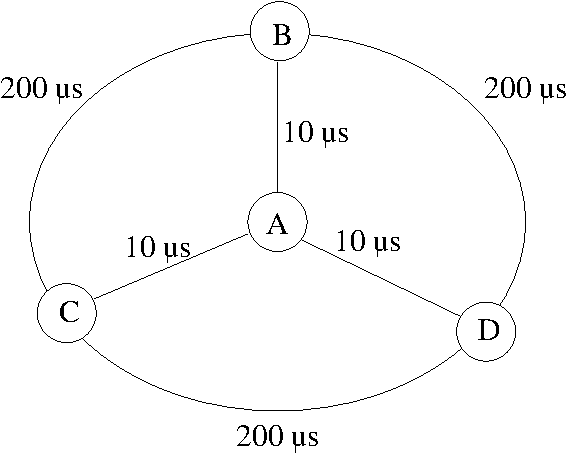
\includegraphics[scale=0.5]{images/topologie/Lowkamp-mistake}
%\par\end{centering}
%
%\caption{\label{Fig:ECOwrong}Contre-exemple à l'algorithme de Lowekamp}
%
%\end{figure}
%
%
%En effet, nous pouvons observer que le noeud A est le seul connecté
%aux autres avec une petite latence. Or, dans ce cas, un groupe \{A,
%B, C, D\} est possible, malgré le fait que l'interconnexion entre
%les noeuds B, C et D est beaucoup plus lente. Dans ce cas, l'hétérogénéité
%des connexions à l'intérieur du groupe peut influencer fortement les
%communications (par exemple, si B devient le coordinateur), sans que
%les modèles de communication soient capables de représenter les performances
%obtenues. Cependant, telles situations sont suffisamment rares pour
%permettre l'utilisation de l'algorithme de Lowekamp dans notre outil
%de découverte de topologie. 
%
%
%\subsection{\label{sec:Getting-pLogP-data}Troisième partie : acquisition efficace
%des paramètres d'interconnexion}
%
%Même si les grappes logiques identifiées par notre \emph{framework}
%présentent la structure effective du réseau, nous ne sommes pas encore
%en mesure de modéliser les communications avec précision. La première
%raison est que la matrice de distances n'est pas totalement remplie.
%Comme expliqué dans la section \ref{sec:First-Phase:-Gathering},
%l'obtention des informations de connectivité se fait localement à
%chaque grappe, et les connexions entre les grappes ne sont pas encore
%établies. 
%
%Une autre raison est que les données obtenues par les outils de surveillance
%du réseau ne sont pas adaptées à nos modèles de communication. Par
%exemple, la latence est obtenue de façon différente par les outils
%NWS \cite{Wolski97} et LogP-MPI \cite{Kielmann00}. Dans le cas de
%NWS, la latence est obtenue directement à partir du temps d'aller-retour
%d'un message. L'outil LogP-MPI, par contre, décompose le temps d'aller-retour
%en deux composants, la latence et le \emph{gap}, comme illustré dans
%la Figure \ref{Figure:Differences-between-NWS}. Les différences entre
%les deux stratégies d'obtention de la latence sont suffisamment grandes
%pour interférer sur la précision des modèles de communication. 
%
%%
%\begin{figure}[h]
%\begin{centering}
%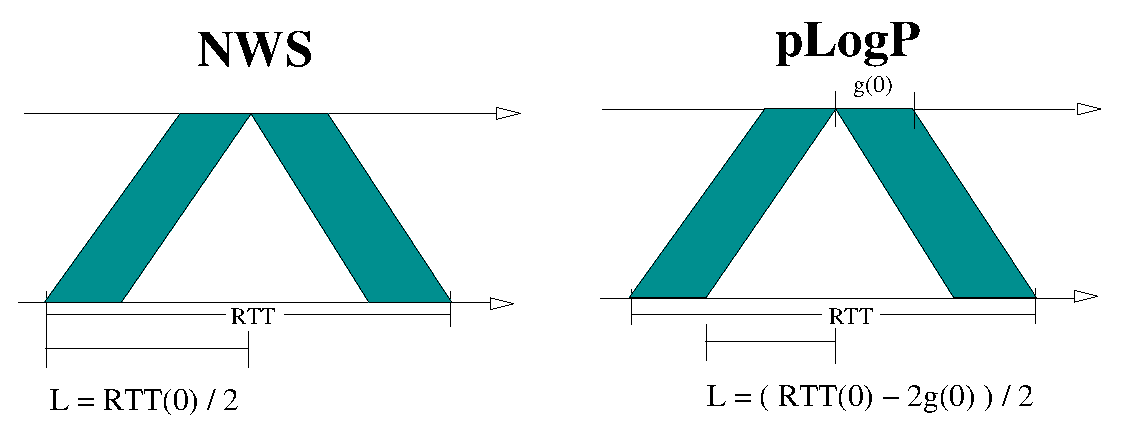
\includegraphics[width=0.9\linewidth,keepaspectratio]{images/topologie/NWSxpLogP}
%\par\end{centering}
%
%\caption{\label{Figure:Differences-between-NWS}Différence entre la latence
%de NWS et de pLogP}
%
%\end{figure}
%
%
%Heureusement, nous n'avons plus besoin d'exécuter $n(n-1)$ mesures,
%une pour chaque interconnexion possible. En effet, l'homogénéité des
%grappes logiques permet qu'une seule mesure des paramètres d'interconnexion
%à l'intérieur de chaque grappe soit suffisante pour représenter toutes
%les communications à l'intérieur cette grappe. De même, il suffirait
%de mesurer une connexion entre chaque grappe pour représenter toutes
%les connexions distantes possibles. 
%
%Finalement, nous pouvons encore réduire le nombre de mesures par moitié,
%si nous considérons que les liens de connexion sont symétriques $a\rightarrow b=b\rightarrow a$.
%Ainsi, se le nombre de grappes logiques identifiées précédemment est
%C, la quantité de mesures est réduite à :
%
%\[
%\frac{C\times(C-1)}{2}+C\]
%
%
%\subsubsection*{Obtention des paramètres}
%
%Comme pLogP est le modèle le plus souple pour représenter les différents algorithmes
%de communication collective, il est aussi important
%de bien obtenir les paramètres nécessaires à ce modèle.
%
%Pour cela, nous avons utilisé la méthode proposée et implantée par
%Kielmann \cite{Kielmann00}. L'avantage de cette méthode par rapport
%à des techniques précédentes comme celles de Culler \cite{Culler96b}
%et Ianello \cite{Ianello97} réside dans l'obtention du paramètre
%\emph{gap}. En effet, les méthodes décrits par Culler et Ianello utilisent
%des grands messages pour saturer le réseau, afin que le débit du lien
%(représenté par le \emph{gap}) soit mesuré. Cependant, cette technique
%est très intrusive et nécessite un temps assez élevé pour mesurer
%le gap dans les réseaux à très haut débit.
%
%Dans l'approche proposé par Kielmann, par contre, le gap est obtenu
%à partir de l'envoi de petits messages de taille zéro. Ainsi, pour
%mesurer \emph{g(0)}, la méthode proposé mesure le temps d'aller-retour
%d'un message de taille zéro - $RTT_{1}(0)$ - entre deux processus,
%\emph{measure} et \emph{mirror}. Ensuite, le nombre de messages envoyés
%simultanés est augmenté, de manière à ce que le temps $RTT_{n}(0)$
%indique le temps nécessaire à l'envoi de \emph{n} messages vers le
%\emph{mirror} suivies d'une unique réponse d'acquittement vers le
%\emph{measure}. Le nombre de messages \emph{n} est doublé jusqu'à
%ce que le \emph{gap} par message ne varie que de d'une marge d'erreur
%$\epsilon$. À ce point, $RTT_{n}(0)$ est considéré comme équivalent
%à \emph{$n\times g(0)$} et la valeur de \emph{$g(0)$} peut être
%facilement obtenue. 
%
%En effet, un premier échange envoie un message de \emph{m} octets,
%qui est répondu par un message de taille zéro (c'est équivalent à
%faire $RTT_{1}(m)$). À partir de $RTT_{1}(m)$, les valeurs de $g(m)$
%et \emph{L} peuvent être déduites directement à partir des équations
%présentées dans le Tableau \ref{Tableau:pLogp_Equations}.
%
%%
%\begin{table}[h]
%	\caption{\label{Tableau:pLogp_Equations}Équations pour l'obtention de $g(m)$
%		avec pLogP \cite{Kielmann00}}
%	
%	
%	\begin{centering}
%		\begin{tabular}{|c|}
%			\hline 
%			$RTT_{1}(0)=2\times(L+g(0))$\tabularnewline
%			$L=(RTT_{1}(0)-2\times g(0))/2$\tabularnewline
%			$RTT_{1}(m)=L+g(m)+L+g(0)$\tabularnewline
%			$g(m)=RTT_{1}(m)-RTT_{1}(0)+g(0)$\tabularnewline
%			\hline
%		\end{tabular}
%		\par\end{centering}
%\end{table}
%
%
%Pour obtenir les autres paramètres comme $o_{s}(m)$ et $o_{r}(m)$,
%nous utilisons la procédure représentée dans la Figure \ref{Figure: pLogP_acquisition}.
%Dans un premier moment, le paramètre $o_{s}(m)$ est obtenu à partir
%de la mesure du temps de l'envoi simple (sans attendre une réponse).
%Dans le deuxième échange de messages, le processus \emph{measure}
%envoie un message de taille zéro et attend pendant un temps $\Delta>RTT_{1}(m)$
%avant de recevoir un message de \emph{m} octets. Cet échange permet
%l'obtention de $o_{r}(m)$, car après le temps $\Delta>RTT_{1}(m)$
%le processus \emph{measure} est certain que le message envoyé par
%\emph{mirror} est déjà disponible dans la mémoire tampon de son interface
%réseau. Il faut observer cependant que cette mesure de $o_{r}(m)$
%n'est correcte que si la communication entre les deux noeuds \emph{measure}
%et \emph{mirror} est symétrique. Si le débit entre \emph{mirror} et
%\emph{measure} est moins important que celui entre \emph{measure}
%et \emph{mirror}, cela peut donner des valeurs de $o_{r}(m)$ plus
%grands que $g(m)$. Ainsi, une manière d'éviter cette situation serait
%de mesurer $o_{r}(m)$ dans une communication \emph{measure-measure},
%si $o_{r}(m)$ est un paramètre essentiel aux modèles étudiés.
%
%%
%\begin{figure}[h]
%	\begin{centering}
%		\includegraphics[width=0.55\linewidth]{images/p2p/pLogP_acquiring}
%		\par\end{centering}
%	
%	\caption{\label{Figure: pLogP_acquisition}Méthode d'obtention des paramètres
%		pLogP \cite{Kielmann00}}
%	
%\end{figure}
%
%
%Répété avec différentes valeurs de \emph{m}, cette procédure permet
%l'obtention de $g(m)$, $o_{s}(m)$ et $o_{r}(m)$ à partir d'un tableau
%contenant une liste d'échantillons, comme présenté dans la Figure
%\ref{Figure:exemple fichier pLogP}. Ces échantillons sont obtenus
%de manière à ce que la détermination des valeurs pour une taille de
%message \emph{m} donnée soit faite à partir de l'interpolation des
%points de mesure les plus proches.
%
%%
%\begin{figure}[h]
%	\begin{centering}
%		{\footnotesize }\begin{tabular}{|l|}
%			\hline 
%			{\footnotesize \texttt{}\foreignlanguage{english}{{\footnotesize \#
%						LogP network performance data: logp\_test-Send-Recv}}{\footnotesize }}\tabularnewline
%			{\footnotesize \texttt{}\foreignlanguage{english}{{\footnotesize \#
%						Latency = 32.66}}{\footnotesize }}\tabularnewline
%			{\footnotesize \texttt{}\foreignlanguage{english}{{\footnotesize \#
%						time }\textbf{\footnotesize bytes}{\footnotesize{} os os\_min os\_cnfint
%						or or\_min or\_cnfint }\textbf{\footnotesize g}}{\footnotesize }}\tabularnewline
%			{\footnotesize \texttt{}\foreignlanguage{english}{{\footnotesize 1113829432
%					}\textbf{\footnotesize 0}{\footnotesize{} 0.0000053 0.0000043 0.0000004
%					0.0000024 0.0000014 0.0000009 }\textbf{\footnotesize 0.0000014}}{\footnotesize }}\tabularnewline
%		{\footnotesize \texttt{}\foreignlanguage{english}{{\footnotesize 1113829432
%				}\textbf{\footnotesize 1}{\footnotesize{} 0.0000056 0.0000043 0.0000005
%				0.0000036 0.0000024 0.0000004 }\textbf{\footnotesize 0.0000035}}{\footnotesize }}\tabularnewline
%	{\footnotesize \texttt{}\foreignlanguage{english}{{\footnotesize 1113829432
%			}\textbf{\footnotesize 2}{\footnotesize{} 0.0000058 0.0000043 0.0000004
%			0.0000038 0.0000033 0.0000010 }\textbf{\footnotesize 0.0000036}}{\footnotesize }}\tabularnewline
%{\footnotesize \texttt{...}}\tabularnewline
%{\footnotesize \texttt{}\foreignlanguage{english}{{\footnotesize 1113829432
%		}\textbf{\footnotesize 256}{\footnotesize{} 0.0000059 0.0000043 0.0000005
%		0.0000042 0.0000033 0.0000007 }\textbf{\footnotesize 0.0000090}}{\footnotesize }}\tabularnewline
%{\footnotesize \texttt{}\foreignlanguage{english}{{\footnotesize 1113829432
%		}\textbf{\footnotesize 512}{\footnotesize{} 0.0000061 0.0000045 0.0000011
%		0.0000041 0.0000033 0.0000009 }\textbf{\footnotesize 0.0000158}}{\footnotesize }}\tabularnewline
%{\footnotesize \texttt{}\foreignlanguage{english}{{\footnotesize 1113829432
%		}\textbf{\footnotesize 1024}{\footnotesize{} 0.0000063 0.0000052 0.0000010
%		0.0000044 0.0000033 0.0000004 }\textbf{\footnotesize 0.0000292}}{\footnotesize }}\tabularnewline
%{\footnotesize \texttt{...}}\tabularnewline
%{\footnotesize \texttt{}\foreignlanguage{english}{{\footnotesize 1113829432
%		}\textbf{\footnotesize 262144}{\footnotesize{} 0.0017727 0.0017314
%		0.0001001 0.0023521 0.0023274 0.0001276 }\textbf{\footnotesize 0.0023500}}{\footnotesize }}\tabularnewline
%{\footnotesize \texttt{}\foreignlanguage{english}{{\footnotesize 1113829433
%		}\textbf{\footnotesize 524288}{\footnotesize{} 0.0039728 0.0038664
%		0.0002125 0.0046024 0.0045595 0.0002578 }\textbf{\footnotesize 0.0045943}}{\footnotesize }}\tabularnewline
%{\footnotesize \texttt{}\foreignlanguage{english}{{\footnotesize 1113829433
%		}\textbf{\footnotesize 1048576}{\footnotesize{} 0.0085095 0.0084665
%		0.0002588 0.0090407 0.0090144 0.0001601 }\textbf{\footnotesize 0.0091020}}{\footnotesize }}\tabularnewline
%{\footnotesize \texttt{...}}\tabularnewline
%\hline
%\end{tabular}{\footnotesize{} }
%\par\end{centering}{\footnotesize \par}
%
%\caption{\label{Figure:exemple fichier pLogP}Exemple d'un tableau avec les
%	paramètres pLogP pour des tailles de message différentes (1 octet
%	jusqu'à 1Mo)}
%
%\end{figure}
%
%
%
%\subsection{\label{sec:Practical Results}Évaluation pratique}
%
%Pour évaluer l'utilisation de notre \emph{framework}, nous avons intégré
%les trois parties de découverte de topologie dans la bibliothèque
%LaPIe, une bibliothèque MPI conçue pour optimiser pour les communications collectives (broadcast, gather, scatter, all-to-all, etc.) dans les environnments de type grille hétérogène. Les deux premières parties du framework sont implantées en une application
%indépendante, alors que la troisième partie est implantée directement dans les
%procédures d'initialisation du MPI.
%
%\subsubsection{Clusterisation}
%
%En effet, les étapes de collecte d'informations et de partitionnement
%des machines ont été regroupées en une application indépendante, exécutée
%par l'utilisateur avant le déploiement de son application, et qui
%fournit un fichier de description des grappes homogènes. Nous avons
%profité des fonctionnalités de la bibliothèque MagPIe, dont nous sommes
%inspirés, pour fournir à l'application une description de la répartition
%des machines qui sera utilisée ensuite pour la construction de la
%topologie des processus. Seule différence, notre bibliothèque a permis
%l'automatisation de la génération de ce fichier de description, ce
%qui est notamment avantageux du point de vue des heuristiques d'optimisation
%qui utilisent cette description.
%
%La troisième partie a été intégrée à la fonction \emph{MPI\_Init},
%appelée à l'initialisation de chaque application MPI. Nous avons intégré
%les fonctions d'obtention des paramètres d'interconnexion aux fonctions
%de description de la topologie. Cela permet notamment la prise en
%charge des coûts de communication réels de l'application.
%
%Pour illustrer notre approche de découverte de topologie, notamment
%la première et la deuxième partie, nous présentons deux expériences,
%l'une sur la grappe IDPOT à Grenoble, et l'autre sur une grille de 78 machines
%réparties entre les sites d'Orsay, Toulouse, Sophia-Antipolis et Grenoble
%(IDPOT). 
%
%La grappe IDPOT était constituée de machines Intel Xeon biprocesseur
%dont une partie des machines utilise des cartes réseau Broadcom Giga
%Ethernet et l'autre partie utilise des cartes réseau Intel Giga Ethernet.
%L'interaction entre les différentes cartes réseau occasionne une forte
%variation de performance des communications, ce qui est très intéressante
%pour les expériences de découverte du réseau (conformément à ce que
%nous avons présenté en \cite{Steffenel04b}). 
%
%À partir de la procédure de découverte de topologie présentée précédemment,
%nous avons pu repartir les machines IDPOT en trois groupes homogènes,
%comme indique la Figure \ref{Figure:exemplefichermagpie_idpot}.
%
%%
%\begin{figure}[h]
%\begin{centering}
%{\footnotesize }\begin{tabular}{|l|}
%\hline 
%{\footnotesize \texttt{cluster 0 }}\tabularnewline
%{\footnotesize \texttt{process 0 1 2 3 6 7 8 9 11 12 17}}\tabularnewline
%{\footnotesize \texttt{cluster 1 }}\tabularnewline
%{\footnotesize \texttt{process 4 5}}\tabularnewline
%{\footnotesize \texttt{cluster 2 }}\tabularnewline
%{\footnotesize \texttt{process 10 13 14 15 16}}\tabularnewline
%{\footnotesize \texttt{\# Min edge 0-0 = 35.524368}}\tabularnewline
%{\footnotesize \texttt{\# Min edge 0-1 = 59.962273}}\tabularnewline
%{\footnotesize \texttt{\# Min edge 0-2 = 59.962273}}\tabularnewline
%{\footnotesize \texttt{\# Min edge 1-1 = 60.439110 }}\tabularnewline
%{\footnotesize \texttt{\# Min edge 1-2 = 122.54715 }}\tabularnewline
%{\footnotesize \texttt{\# Min edge 2-2 = 60.081482 }}\tabularnewline
%\hline
%\end{tabular}{\footnotesize{} }
%\par\end{centering}{\footnotesize \par}
%
%\caption{\label{Figure:exemplefichermagpie_idpot}Fichier de description de
%grappes logique homogènes pour le réseau IDPOT, avec la latence entre
%les grappes (microsecondes)}
%
%\end{figure}
%
%
%Cette différence entre les machines IDPOT se reflète aussi sur le
%gap, comme indiqué dans le Tableau \ref{Tableau :Gap-IDPOT}, malgré
%le fait que les machines appartiennent toutes au même sous-réseau
%IP, technique normalement utilisée pour regrouper les machines. 
%
%En effet, une telle variation des valeurs des paramètres d'interconnexion
%(le gap et la latence) ne permet pas une prédiction de performance
%très précise, car les modèles de performance considèrent que le réseau
%est uniforme, c'est-à-dire, une valeur unique de gap et latence pour
%tout le réseau. À l'aide de notre outil pour la découverte de topologie
%nous pouvons alors identifier les sous-réseaux homogènes et les traiter
%séparément, de manière, par exemple, à réorganiser les communications
%selon les heuristiques présentées dans le chapitre \ref{cha:Comm sur grille}.
%En conséquence, l'identification des sous-réseaux homogènes rend possible
%une meilleure modélisation du réseau réel que le simple regroupement
%des noeuds par localisation ou sous-réseau IP.
%
%%
%\begin{table}
%\caption{\label{Tableau :Gap-IDPOT}Gap pour un message de 1Mo sur les sous-réseaux
%IDPOT, en millisecondes}
%
%
%\begin{centering}
%\begin{tabular}{|c||c|c|c|}
%\hline 
% & sous-réseau 0 & sous-réseau 1 & sous-réseau 2\tabularnewline
%\hline
%\hline 
%sous-réseau 0 & 9,0906 & 19,7898 & 16,4515\tabularnewline
%\hline 
%sous-réseau 1 & 19,7898 & 25,0942 & 25,2701\tabularnewline
%\hline 
%sous-réseau 2 & 16,4515 & 25,2701 & 26,1203\tabularnewline
%\hline
%\end{tabular}
%\par\end{centering}
%\end{table}
%
%
%La deuxième expérience réalisée considère une grille de 78 machines,
%dont 20 machines de la grappe GdX d'Orsay, 20 machines de la grappe
%de Toulouse, 19 machines de la grappe de Sophia-Antipolis et 17 machines
%de la grappe IDPOT.
%
%À l'aide de notre application de découverte de topologie (appelée
%\emph{subnets}), nous pouvons obtenir un fichier de description de
%la topologie similaire à celui présenté dans la Figure \ref{Figure:exemplefichermagpie_clusters}.
%
%%
%\begin{figure}[h]
%\begin{centering}
%{\footnotesize }\begin{tabular}{|l|}
%\hline 
%{\footnotesize \texttt{cluster 0 }}\tabularnewline
%{\footnotesize \texttt{process 0 1 2 3 4 5 6 7 8 9 10 11 12 13 14
%15 16 17 18 19 }}\tabularnewline
%{\footnotesize \texttt{cluster 1 }}\tabularnewline
%{\footnotesize \texttt{process 20 21 22 23 26 28 29 30 32 33 38 }}\tabularnewline
%{\footnotesize \texttt{cluster 2 }}\tabularnewline
%{\footnotesize \texttt{process 24 25 27 31 34 35 37 }}\tabularnewline
%{\footnotesize \texttt{cluster 3 }}\tabularnewline
%{\footnotesize \texttt{process 36 }}\tabularnewline
%{\footnotesize \texttt{cluster 4 }}\tabularnewline
%{\footnotesize \texttt{process 39 40 41 42 43 44 45 46 47 48 49 50
%51 52 53 54 55 56 57 58 }}\tabularnewline
%{\footnotesize \texttt{cluster 5}}\tabularnewline
%{\footnotesize \texttt{process 59 60 61 62 63 64 65 66 67 68 69 70
%71 72 73 74 75 76 77 }}\tabularnewline
%\hline
%\end{tabular}{\footnotesize{} }
%\par\end{centering}{\footnotesize \par}
%
%\caption{\label{Figure:exemplefichermagpie_clusters}Fichier de description
%de grappes logique homogènes}
%
%\end{figure}
%
%
%Il faut noter que les machines sont identifiées par le rang du processus
%MPI ; pour mieux identifier l'appartenance de chaque machine, nous
%présentons dans la Figure \ref{Figure: Topo Grille 78 machines} la
%distribution des six grappes homogènes par rapport à la localisation
%de ces machines.
%
%%
%\begin{figure}[h]
%\begin{centering}
%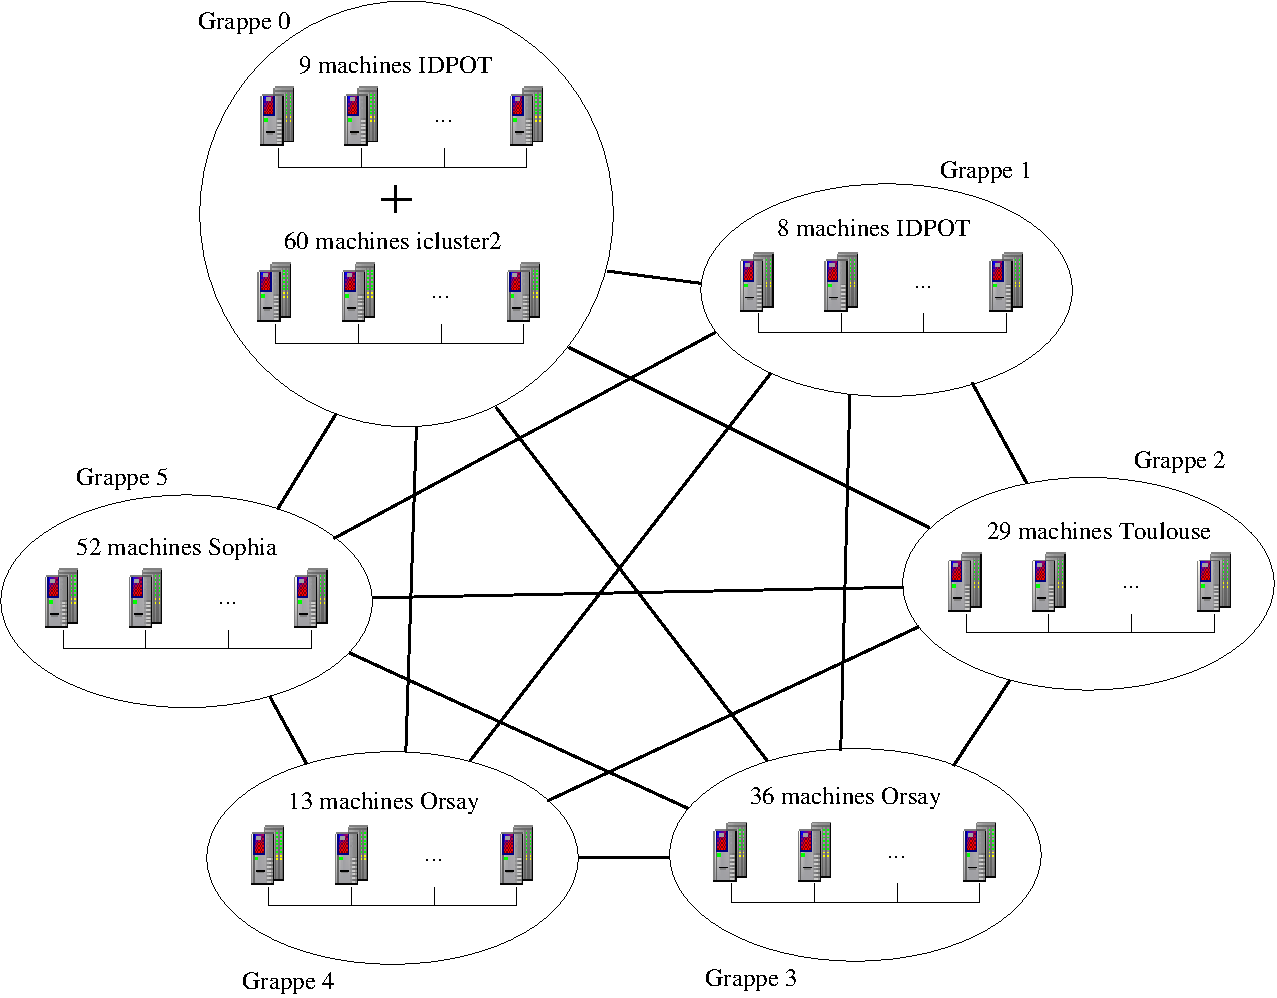
\includegraphics[width=0.75\linewidth]{images/Grid/Bcast/case2/grappe-case2}
%\par\end{centering}
%
%\caption{\label{Figure: Topo Grille 78 machines}Répartition des grappes homogènes
%dans une grille de 78 machines }
%
%\end{figure}
%
%
%Dans cet environnement, l'hétérogénéité est majoritairement due au
%facteur géographique. Cependant, le facteur matériel est aussi important,
%comme illustré par les machines du réseau IDPOT. Dans ce cas, nous
%observons que certaines machines peuvent être regroupées en grappes
%différentes malgré leur proximité géographique. Ainsi, les latences
%d'interconnexion entre les différents sites sont présentées dans le
%Tableau \ref{Tableau: topo case 2 latences}. On observe que malgré
%le seuil de tolérance de 30\% utilisée par l'algorithme de partitionnement,
%la différence entre les machines IDPOT est suffisamment élevée pour
%forcer le regroupement des machines en différentes grappes.
%
%%
%\begin{table}[h]
%\caption{\label{Tableau: topo case 2 latences}Latence entre les différents
%sites (en microsecondes)}
%
%
%\begin{centering}
%{\footnotesize }\begin{tabular}{|c||c|c|c|c|c|c|}
%\hline 
% & {\footnotesize Grappe 0} & {\footnotesize Grappe 1} & {\footnotesize Grappe 2} & {\footnotesize Grappe 3} & {\footnotesize Grappe 4} & {\footnotesize Grappe 5}\tabularnewline
%\hline 
% & {\footnotesize 20 x Orsay} & {\footnotesize 11 x IDPOT} & {\footnotesize 7 x IDPOT} & {\footnotesize 1 x IDPOT} & {\footnotesize 20 x Toulouse} & {\footnotesize 19 x Sophia}\tabularnewline
%\hline
%\hline 
%{\footnotesize Grappe 0} & {\footnotesize 48.39} & {\footnotesize 6577.49} & {\footnotesize 6586.49} & {\footnotesize 6592.51} & {\footnotesize 5211.94} & {\footnotesize 8602.73}\tabularnewline
%\hline 
%{\footnotesize Grappe 1} & {\footnotesize 6577.49} & {\footnotesize 35.52} & {\footnotesize 59.96} & {\footnotesize 59.96} & {\footnotesize 5387.48} & {\footnotesize 2736.56}\tabularnewline
%\hline 
%{\footnotesize Grappe 2} & {\footnotesize 6586.49} & {\footnotesize 59.96} & {\footnotesize 60.08} & {\footnotesize 79.51} & {\footnotesize 5393.98} & {\footnotesize 2740.26}\tabularnewline
%\hline 
%{\footnotesize Grappe 3} & {\footnotesize 6592.51} & {\footnotesize 59.96} & {\footnotesize 79.51} & {\footnotesize 0$^{*}$} & {\footnotesize 5405.78} & {\footnotesize 2745.98}\tabularnewline
%\hline 
%{\footnotesize Grappe 4} & {\footnotesize 5211.94} & {\footnotesize 5387.48} & {\footnotesize 5393.98} & {\footnotesize 5405.78} & {\footnotesize 26.94} & {\footnotesize 3630.51}\tabularnewline
%\hline 
%{\footnotesize Grappe 5} & {\footnotesize 8602.73} & {\footnotesize 2736.56} & {\footnotesize 2740.26} & {\footnotesize 2745.98} & {\footnotesize 3630.51} & {\footnotesize 35.04}\tabularnewline
%\hline
%\end{tabular}
%\par\end{centering}{\footnotesize \par}
%
%\begin{centering}
%{\footnotesize {*} cette grappe contient une seule machine.}
%\par\end{centering}
%\end{table}
%
%
%La dernière partie de notre \emph{framework} de découverte de topologie
%est dédiée à l'obtention des paramètres d'interconnexion, nécessaires
%à la modélisation des communications. Cette partie est exécutée à
%l'initialisation de l'application, à partir des informations préliminaires
%fournies par le fichier de description de la topologie du réseau obtenu
%précédemment. Comme la procédure de mesure des paramètres peut demander
%un temps non négligeable, nous avons l'intérêt en minimiser le temps
%d'obtention des paramètres pour ne pas trop gêner l'utilisateur. À
%l'aide de notre \emph{framework} de découverte de topologie, le nombre
%de mesures est naturellement réduit grâce au regroupement des machines
%en grappes logique homogènes. Dans le cas de notre exemple, le nombre
%de mesures nécessaires est seulement 21 ($(C\times(C-1))/2+C$), ce
%qui représente moins de 1\% du nombre total d'interconnexions ($n\times(n-1)/2$).
%En plus, nous utilisons un algorithme d'ordonnancement pour que ces
%21 mesures soient effectuées, dans la mesure du possible, de manière
%parallèle. 

\section{Modélisation de MPI\_Broadcast dans une Grille}

%Plusieurs travaux récents visent l'implémentation des opérations de
%communication collective adaptées aux systèmes à grande échelle, notamment
%les grilles. Dans ces environnements, l'hétérogénéité est un facteur
%prépondérant qui doit obligatoirement être pris en compte, comme nous
%l'avons déjà observé \cite{Barchet04b}. Cette hétérogénéité représente
%néanmoins un vrai défi pour la prédiction des performances, car les
%facteurs qui influencent les communications ont des origines très
%variées, comme la distribution des processus (par exemple, sur une
%grappe de machines multiprocesseurs), la distance entre les machines
%et/ou les grappes, le taux d'utilisation du matériel (surtout la congestion
%du réseau) et la variation de performance du matériel. En effet, les
%grilles de calcul combinent, la plupart du temps, différentes machines
%et réseaux.
%
%L'hétérogénéité inhérente à ces environnements, associée à la volatilité
%des noeuds dans les grilles de calcul, empêche la création d'opérations
%spécifiques pour ces environnements, comme en attestent \cite{Bhat03}
%et \cite{Vadhiyar00}. Pour simplifier cette modélisation, la plupart
%des solutions considèrent les grilles comme l'interconnexion d'îlots
%de grappes homogènes. Dans ce contexte, la majorité des systèmes concentre
%l'optimisation au niveau des communications entre les grappes, puisque
%ces liaisons sont généralement plus lentes que celles intérieures
%à la grappe. Quelques exemples de cette approche en deux couches incluent
%les bibliothèques ECO \cite{Lowekamp96}, MagPIe \cite{Kielmann99b}\cite{Kielmann01},
%et même la bibliothèque LAM-MPI 7 \cite{LAM04}, qui considère les
%machines SMP comme des îlots de communication rapide. Il reste néanmoins
%la nécessité de régler les paramètres de communication pour avoir
%des performances optimales. Pour cela, la prédiction des performances
%à travers des modèles de communications est un choix très avantageux.
%
%Il existe toutefois la possibilité d'organiser les communications
%en un plus grand nombre de couches. En effet, le travail de Karonis
%et \emph{al.} \cite{Karonis00}\cite{Karonis02} a démontré que le
%découpage en plusieurs couches de communication peut conduire à des
%réductions du temps d'exécution plus importantes qu'un découpage en
%deux couches. Cependant, il est nécessaire de connaître \emph{a priori}
%le coût de communication interne à chaque grappe. Dans ce cas, le
%calcul de la distribution et de la hiérarchie des communications dépend
%des temps de communication à l'intérieur des grappes. Ces temps varient
%selon l'opération de communication collective, le nombre de noeuds
%et les caractéristiques du réseau de chaque grappe. 
%
%
%\subsubsection{État de l'art}

L'opération \emph{Broadcast} est une des plus simples opérations de
communication collective : initialement, seul le processus \emph{racine}
détient le message qui doit être diffusé ; à la fin de l'opération,
une copie de ce message est déposée dans chaque processus du groupe.
La détermination du meilleur arbre de diffusion pour un environnement
homogène est une tâche relativement facile : le choix de l'arbre dépend
surtout des paramètres d'interconnexion.

Cependant, dans le cas d'un réseau hétérogène, ce problème devient
bien plus difficile : en effet, l'identification du meilleur arbre
de diffusion est un problème NP-complet \cite{Bhat99}\cite{Beaumont04c,Beaumont05b}\cite{PangfengLiu04}.

%En raison de ces restrictions, plusieurs travaux s'intéressent au
%développement de techniques d'approximation qui soient suffisamment
%efficaces pour être utilisées dans un système réel. Parmi ces travaux
%on note celui de Beaumont \emph{et al.} \cite{Beaumont04c,Beaumont05b},
%Banikazemi \cite{Banikazemi98}, Bhat \cite{Bhat99,Bhat03}, Liu \cite{Liu03},
%Park \cite{Park96}, Mateescu \cite{Mateescu05}, Miled \cite{Miled98}
%et Vorakosit \cite{Vorakosit03}. L'approche de Beaumont utilise des
%algorithmes de type \og \emph{prunning} \fg{} pour identifier le
%meilleur arbre de diffusion possible à l'intérieur d'un réseau, alors
%que la plupart des travaux font la construction d'un arbre de diffusion
%à partir d'une source donnée. L'approche \emph{\og prunning \fg{}}
%est plus adaptée à une diffusion en régime continu, comme par exemple
%la transmission d'un flux multimédia. Leurs efforts sont alors concentrés
%sur l'optimisation du débit maximal atteint. 
%
%L'approche la plus générale, utilisée par les autres auteurs cités
%ci-dessus (Banikazemi, Bhat, Vorakosit, etc.), utilise comme processus
%racine un processus indiqué par l'utilisateur. Cette approche est
%plutôt orientée vers des diffusions occasionnelles où la source du
%broadcast peut changer d'un appel à l'autre. Ce modèle correspond
%plus exactement au format de l'appel MPI\_Bcast.

La plupart des travaux dédiés à l'optimisation des communications
collectives dans des environnements hétérogènes font référence aux
processus communicants. C'est-à-dire, les optimisations sont faites
en tenant compte du coût d'interconnexion entre chaque paire de processus
concernée par le broadcast. C'est le cas de Banikazemi \cite{Banikazemi98},
Bhat \cite{Bhat99,Bhat03} et Mateescu \cite{Mateescu05}, qui utilisent
différentes stratégies pour construire des arbres de diffusion optimisés.

Cependant, l'environnement de type grille est normalement caractérisé
par un grand nombre de processus communicants, résultat de l'association
des différentes grappes de calcul. Dans ce cas, la complexité de la
tâche d'optimisation est bien plus importante, et des simplifications
s'imposent afin de permettre l'utilisation de telles méthodes dans
la pratique. Une de ces simplifications est le regroupement des processus
selon leurs performances relatives (par exemple, par rapport à la
communication), de manière à ce que toute une classe de processus
puisse être traitée comme une entité unique. De cette manière, l'augmentation
massive du nombre de processus dans une grille de calcul peut être
encore facilement abordable par les méthodes d'optimisation classiques, i.e., la division des communications en deux couches, l'\textit{inter-grappes} et l'\textit{intra-grappes}. 

%Toutefois, cette simplification au niveau de l'optimisation requiert
%en contrepartie l'organisation des différentes classes de processus
%autour d'un ou plusieurs \og coordinateurs \fg{}. Ces derniers sont
%des processus responsables de la communication avec les autres grappes
%et de la diffusion à l'intérieur du groupe de processus. Cette organisation
%des processus assume tout naturellement une disposition hiérarchique,
%où les messages sont diffusés d'abord entre les coordinateurs des
%groupes, et finalement vers les autres processus.
%
%L'un des premiers travaux à adresser ce problème pour les grilles
%est celui de Lowekamp \cite{Lowekamp96,Lowekamp00}, où les machines
%sont regroupées selon leur localisation dans le réseau. Le même principe
%est suivi par la bibliothèque MagPIe \cite{Kielmann99b}, de manière
%à ce que les échanges de messages à travers les liens plus lents (ceux
%qui connectent les différentes grappes) soient réduits au minimum. 
%
%Une caractéristique commune à ces deux travaux est que la communication
%se fait en deux couches, l'\emph{inter-grappes} et l'\emph{intra-grappes}.
%Si cette disposition permet la minimisation du trafic sur les liens
%les plus lents, elle ne tire pas partie des caractéristiques du Broadcast
%comme la multiplication des sources de diffusion, principe de base
%du Broadcast en systèmes homogènes. Karonis \cite{Karonis00,Karonis02}
%a adressé ce problème en établissant des communications à plusieurs
%niveaux, de manière à permettre le recouvrement des communications
%des différentes grappes et à minimiser le temps de diffusion inter-grappes.
%Cependant, l'approche de Karonis est purement orientée par la latence
%de communication, et comme l'atteste Lacour \cite{Lacour01}, l'implémentation
%de MPICH-G2 identifie les différents niveaux selon leurs latences
%relatives (cf. Tableau \ref{Tableau: niveaux mpichg2}). De cette
%manière, la communication entre différentes grappes (niveaux 0 et
%1) est établie de façon similaire au modèle en deux couches, ce qui
%ne permet pas une véritable amélioration par rapport au modèle de
%MagPIe.

%%
%\begin{table}[h]
%	\caption{\label{Tableau: niveaux mpichg2}Ordre des niveaux selon la latence
%		des protocoles de communication \cite{Lacour01}}
%	
%	
%	\begin{centering}
%		\begin{tabular}{|c|c|c|c|}
%			\hline 
%			Niveau 0 > & Niveau 1 > & Niveau 2 > & Niveau 3, 4, ...\tabularnewline
%			\hline
%			\hline 
%			&  &  & mémoire partagée\tabularnewline
%			WAN-TCP & LAN-TCP & localhost-TCP & Myrinet\tabularnewline
%			&  &  & MPI fabricants\tabularnewline
%			\hline
%		\end{tabular}
%		\par\end{centering}
%\end{table}


Cependant, à défaut de leur apport aux algorithmes de Broadcast, ces
techniques peuvent être améliorées. En effet, les travaux précédents
ont été établis dans un contexte où les communications de longue distance
étaient plusieurs ordres plus lentes que celles à l'intérieur des
réseaux locaux, et la réduction des communications inter-grappes permettait
la minimisation de la congestion sur les liens les plus lents. Si
cela est encore vrai en ce qui concerne la latence entre les noeuds,
il n'est plus exact pour le débit d'un lien de longue distance. D'autre
part, le faible coût du matériel informatique permet aujourd'hui que
les grappes regroupent des centaines de noeuds. Or, plus le coût de
diffusion \og intra-grappes \fg{} devient important, plus son influence
sur la performance sera importante au moment de définir l'ordonnancement
des communications.

C'est exactement ce qui différencie les heuristiques traitant (ou
ne traitant pas) la communication à l'intérieur des groupes : les
heuristiques \og traditionnelles \fg{} et celle appelées \og heuristiques
sensibles au contexte des grilles de calcul \fg{} (\og \emph{grid-aware} \fg{}
en anglais). Dans le premier cas, l'optimisation ne tient compte que
des communications entre les différents coordinateurs, alors que le
deuxième cas s'occupe aussi de la diffusion à l'intérieur des grappes. 

%Afin de permettre une optimisation moins centrée sur la latence, et
%qui fait aussi usage des autres paramètres de connexion dont nous
%disposons, nous avons étudié certaines heuristiques proposées par
%Banikazemi \cite{Banikazemi98}, Bhat \cite{Bhat03} et Liu \cite{Liu02},
%proposées initialement dans le cadre des réseaux hétérogènes. Ces
%heuristiques ont pour objectif la construction d'arbres de diffusion
%(à travers l'ordonnancement des communications) qui minimisent le
%temps de complétion du Broadcast. Alors que ces heuristiques peuvent
%être utilisées pour la construction d'un arbre de diffusion complet,
%cela implique une augmentation de la complexité des optimisations
%qui parfois n'est pas justifiée, comme par exemple dans le cas des
%réseaux homogènes, dont nous connaissons déjà la meilleure stratégie
%de diffusion (conformément à ce qui a été présenté en chapitre \ref{cha:Mod=0000E9lisation des comms collectives}).
%C'est pour cette raison que nous avons utilisé ces heuristiques seulement
%pour structurer la communication inter-grappes, intrinsèquement hétérogène.

Les prochaines sections présentent les différentes heuristiques étudiées
pour l'optimisation des communications de type MPI\_Bcast. Certaines
de ces heuristiques sont la simple application des méthodes pour les
réseaux hétérogènes dans le contexte des grappes hiérarchisées. Dans
ce travail nous proposons trois nouvelles méthodes, qui au contraire
des techniques précédentes, considèrent autant les communications
entre les coordinateurs que les temps nécessaires à la diffusion des
messages à l'intérieur des grappes.


\subsubsection*{Formalisme utilisé}

Pour décrire les heuristiques présentées dans cette section, nous
utilisons un formalisme de groupes similaire à celui de Bhat \cite{Bhat03}.
Dans ce formalisme, les grappes sont séparées en deux groupes, \textbf{A}
et \textbf{B}. Le groupe \textbf{A} contient les grappes qui ont déjà
reçu le message (la réception du message par le coordinateur de la
grappe est suffisante). Le groupe \textbf{B} contient les grappes
qui devront recevoir le message. De cette manière, le groupe \textbf{A}
contient initialement la grappe du processus \emph{source} ou \emph{racine},
tandis que le groupe \textbf{B} contient toutes les autres grappes
du réseau.

À chaque étape, un émetteur appartenant au groupe \textbf{A} et un
récepteur appartenant au groupe \textbf{B} sont choisis. Après la
communication entre ces deux grappes (plus exactement, leurs coordinateurs),
la grappe réceptrice est transférée au groupe \textbf{A}. 

L'implémentation de ces communications est faite de manière à rendre
prioritaires les communications entre les grappes. En effet, les coordinateurs
diffusent le message à l'intérieur de ses grappes seulement après
la fin des communications inter-grappes. Cette stratégie favorise
la multiplication des sources disponibles et l'application des heuristiques,
ainsi que la prédiction du temps total d'exécution du Broadcast.


\subsubsection*{Diffusion en Arbre Plat (Flat)}

L'heuristique en \emph{Arbre Plat} (approche utilisée par la bibliothèque
MagPIe), découpe la communication en deux niveaux, \emph{inter-grappes}
et \emph{intra-grappes}. 

Dans le premier niveau, le processus \emph{racine} envoie le message
à tous les coordinateurs des différentes grappes. L'ordre d'envoi
suit le \og rang \fg{} des différentes grappes, prédéfini à l'initialisation
de MagPIe (normalement, à travers le fichier \emph{magpie\_clusters}).
Formellement, cela veut dire qu'à chaque étape, le processus \emph{racine}
choisi comme récepteur la première grappe du groupe \textbf{B}. Dans
cette \og heuristique \fg{}, le processus émetteur est toujours
le même (le processus \emph{racine}), malgré le fait que les grappes
qui ont déjà reçu le message font désormais partie du groupe \textbf{A}.
Dans le deuxième niveau de diffusion, exécuté à l'intérieur de chaque
grappe, les coordinateurs exécutent un \emph{broadcast} en arbre binomial.

Même si cette heuristique est très simple à implanter, elle est toutefois
très peu optimisée. En effet, la diffusion des données ne tient pas
compte des performances des différentes grappes, ni les vitesses d'interconnexion
entre les \emph{coordinateurs}. Même si l'utilisateur organise le
fichier de description des grappes de manière à favoriser les communications
émises d'une certaine grappe, celles-ci restent soumises à une structure
de diffusion \emph{plate}. 


\subsubsection*{Fastest Node First - FNF}

L'heuristique \emph{Fastest Node First} (le noeud le plus rapide d'abord)
a été proposée par Banikazemi \emph{et al.} \cite{Banikazemi98}.
Dans leur modèle de communication, le réseau est composé d'un certain
nombre de noeuds \emph{$P$}. À chaque noeud \emph{$P_{\textrm{i}}$}
on associe un coût d'envoi \emph{$C_{\textrm{i}}$}. Ce coût \emph{$C_{\textrm{i}}$}
est indépendant de la destination et de la taille du message, et indique
seulement la différence de vitesse entre les noeuds.

L'heuristique proposée par Banikazemi \emph{et al.} nécessite $P-1$
itérations, où à chaque étape l'heuristique définie un émetteur et
un récepteur. Le récepteur est choisi parmi les possibles récepteurs
du groupe \textbf{B} dont le coût \emph{$C_{\textrm{i}}$} est le
plus petit. L'émetteur est le processus du groupe \textbf{A} qui peut
finir la communication le plus rapidement possible. Cela dit, cette
stratégie choisit l'émetteur le plus rapide et le récepteur qui pourrait
retransmettre les messages le plus rapidement possible, à son tour.

L'efficacité de l'heuristique FNF dans le cadre des environnements
homogènes a été démontrée par Liu \cite{PangfengLiu00b}, qui a prouvé que
l'heuristique FNF produit des ordonnancements avec au plus deux fois
le temps optimal.

Cependant, des environnements homogènes comme ceux considérés par
Banikazemi sont assez rares dans les grilles, ce qui rend cette heuristique
très limitée par rapport à la modélisation des communications. En
effet, le modèle de coût unique $C_{\textrm{i}}$ n'est pas suffisant
pour représenter l'hétérogénéité d'un réseau d'interconnexion, comme
indiqué par Bhat \cite{Bhat03}. 


\subsubsection*{Fastest Edge First - FEF}

Proposée par Bhat \emph{et al.} \cite{Bhat03}, l'heuristique \emph{Fastest
	Edge First} (l'arête la plus rapide d'abord) est un algorithme glouton
qui fait partie d'une collection d'heuristiques proposées comme alternative
à l'heuristique FNF. 

Assez simple, cette heuristique est très similaire à l'heuristique
FNF. Seulement, au lieu d'un coût de communication unique $C_{\textrm{i}}$,
l'heuristique évalue le poids de chaque lien de communication $L_{i,j}$
entre deux noeuds différents (les arêtes), correspondants à la latence
de communication entre les deux processus. 

Pour identifier l'ordonnancement des communications nécessaire à l'exécution
de l'opération de Broadcast, l'algorithme FEF, ordonne les processus
du groupe A selon leurs arêtes les plus rapides. Cela permet le choix
du lien le plus rapide parmi toutes les possibilités, et en même temps,
sert à définir l'émetteur et le récepteur, déterminés implicitement
par l'arête choisie. Une fois que le récepteur est désigné, celui-ci
est transféré du groupe \textbf{B} vers le groupe \textbf{A}. À cet
instant, les arêtes minimales doivent être recalculées.

Le raisonnement de cette heuristique est que le choix des liens les
plus rapides permet d'augmenter rapidement le nombre d'émetteurs.
À leur tour, ces émetteurs pourront disséminer le message vers les
processus les plus éloignés, tout en choisissant le lien le moins
coûteux.


\subsubsection*{Early Completion Edge First - ECEF}

Selon les heuristiques précédentes, une fois que le récepteur était
assigné, celui-ci était immédiatement transféré vers le groupe des
émetteurs, le groupe \textbf{A}. Toutefois, à cause des délais de
communication, il est possible que ce récepteur n'ait pas encore reçu
le message et qu'il soit choisi pour le retransmettre à un deuxième
processus. La communication subira un retard supplémentaire, alors
qu'une autre arête, moins rapide, pourrait finir la transmission plus
vite si son émetteur a déjà le message. 

Pour tenir compte des retards dus à la transmission des données, l'heuristique
\emph{Early Completion Edge First} (arête qui finit le plus tôt) considère
aussi dans son évaluation l'instant où les émetteurs ont les données
disponibles pour l'envoi. Ainsi, la \emph{disponibilité} $RT_{i}$
du processus émetteur (\emph{Ready Time} en anglais) est alors utilisée
conjointement avec le temps nécessaire à la transmission du message
entre les processus (le gap plus la latence) de manière à choisir
le couple émetteur-récepteur qui minimise le temps : 

\[
RT_{i}+g_{i,j}(m)+L_{i,j}\]


Ainsi, l'objectif de cette heuristique est d'augmenter le nombre de
processus qui peuvent \emph{effectivement} transmettre les messages
aux autres processus.


\subsubsection*{Early Completion Edge First with lookahead - ECEF-LA}

Pour augmenter l'efficacité de l'heuristique précédente, la dernière
heuristique proposée par Bhat \emph{et al.} \cite{Bhat03} propose
une recherche plus approfondie sur les possibles choix. En effet,
si l'objectif des heuristiques précédentes était la multiplication
des sources disponibles, cela suppose que ces sources pourront, à
leur tour, retransmettre les messages de manière efficace.

C'est ainsi que Bhat a proposé l'utilisation d'une fonction de \emph{lookahead}
(recherche en avant) pour évaluer si le choix d'un récepteur est réellement
bon. De cette manière, l'algorithme calcule préalablement la fonction
de \emph{lookahead} $F_{j}$ pour tous les processus dans le groupe
\textbf{B}, et la paire émetteur-récepteur est celle qui minimise
la somme :

\[
RT_{i}+g_{i,j}(m)+L_{i,j}+F_{j}\]


Cette fonction de \emph{lookahead} peut être définie de plusieurs
façons. Bhat \cite{Bhat03} propose, par exemple, le coût minimal
pour que le processus \emph{j} transmette à d'autres processus encore
dans le groupe \textbf{B}. Cette fonction est alors la suivante :

\begin{eqnarray*}
	F_{j} & = & \min_{P_{k}\in B}\,(g_{j,k}(m)+L_{j,k})\end{eqnarray*}


Intuitivement, cette fonction indique l'utilité du processus $P_{j}$
si à son tour il est transféré vers le groupe \textbf{A}. D'ailleurs,
Bhat a proposé d'autres fonctions de \emph{lookahead}, dont par exemple
la moyenne de la latence entre $P_{j}$ et les autres processus en
\textbf{B}, ou alors la latence moyenne entre les émetteurs et les
récepteurs, si on considère que $P_{j}$ est transféré vers le groupe
\textbf{A}. 


\subsection*{Heuristiques "sensibles au contexte des grilles de calcul"}

Si parmi les heuristiques présentées précédemment nous avons déjà
hiérarchisé les communications en deux niveaux - \emph{inter-grappes}
et \emph{intra-grappes} - , jusqu'à présent les fonctions d'évaluation
ne tiennent compte que des coûts de transmission entre les coordinateurs
des différentes grappes du réseau.

Cependant, comme nous l'avons déjà exposé, le coût d'une communication
hiérarchique ne dépend pas seulement des latences entre les différentes
grappes, mais aussi du temps nécessaire à la diffusion des messages
à l'intérieur de ces grappes. Ce coût de diffusion intra-grappes devient
encore plus important avec l'augmentation du nombre de noeuds à l'intérieur
des grappes, qui aujourd'hui dépasse facilement la centaine de machines.
Par exemple, l'envoi d'un message de 1Mo entre les grappes \emph{Grid
	eXplorer} et \emph{icluster-2} requiert 349 millisecondes, alors que
le broadcast de ce même message entre 50 noeuds de la grappe \emph{icluster-2}
peut nécessiter jusqu'à 3 secondes selon le réseau et l'algorithme
utilisé. Si ce temps n'est pas pris en compte lors de la modélisation
des communications, l'ordonnancement des communications risque d'être
sous-optimal.

Plus exactement, le temps de diffusion intra-grappes, appelé $T_{k}$,
correspond aux prédictions des modèles de communication. Ce temps
est obtenu grâce aux modèles présentés en chapitre \ref{cha:Mod=0000E9lisation des comms collectives}.
Cette notation $T_{k}$ est équivalente à une notation où un noeud
fictif $k'$ est associé à chaque coordinateur $k$, dont :

\[
L_{k,k'}+g_{k,k'}=\left\{ \begin{array}{c}
\begin{array}{cc}
T_{k} & si\: k'\, est\, associe\, a\, k\\
\infty & \,\,\,\,\,\,\,\,\,\,\,\,\, pour\, tout\, autre\, processus\, j\neq k\end{array}\end{array}\right.\]


Alors que les deux notations sont équivalentes, chacune a des avantages
: l'adjonction d'un noeud fictif permet l'utilisation des heuristiques
précédentes sans la nécessité d'une modification des algorithmes,
notamment le ECEF. L'utilisation de $T_{k}$ permet une implémentation
plus simple des algorithmes, qui n'ont pas besoin de garder les deux
identités \emph{k} et \emph{k'} associées à une grappe \emph{k}. Si
ces deux notations sont facilement transformées, nous avons gardé
toutefois la description séparée \emph{L}, \emph{g} et \emph{T}, afin
de permettre une identification plus facile des facteurs évalués.

Dans ce sens, nous présentons deux nouvelles stratégies d'évaluation
dites \og sensibles au contexte des grilles de calcul \fg{}, où
le temps de diffusion \emph{intra-grappe} est aussi considéré lors
de la construction des arbres de diffusion. Pour mieux analyser l'efficacité
de ces stratégies, nous avons aussi développé une version de l'heuristique
ECEF-LA où le temps intra-grappes est pris en compte. Cette version
sert de comparaison par rapport aux heuristiques de Bhat, présentées
précédemment. 


\subsubsection*{ECEF-LA\emph{t}}

L'heuristique ECEF-LA\emph{t} est l'évolution naturelle de l'heuristique
ECEF-LA où nous utilisons une fonction de \emph{lookahead} adaptée
à la représentation du coût de communication intra-grappes $T_{k}$. 

Ainsi, l'heuristique ECEF-LA\emph{t} cherche à minimiser le coût total
de transmission et le temps nécessaire à la diffusion d'un message
dans une grappe distante (en effet, le \og petit \emph{t} \fg{}
du nom de cette heuristique indique qu'on cherche le minimum des temps).
Pour cela, elle utilise une fonction d'évaluation :

\begin{eqnarray*}
	F_{j} & = & \min_{P_{k}\in B}\,(g_{j,k}(m)+L_{j,k}+T_{k})\end{eqnarray*}


À l'instar de l'heuristique ECEF-LA, le but de cette stratégie est
que le récepteur soit choisi parmi les grappes qui peuvent retransmettre
le message le plus vite possible à d'autres grappes. L'adjonction
du temps $T_{k}$ dans la fonction d'évaluation implique aussi que
le choix d'un interlocuteur minimisera le temps de complétion des
grappes contactées dans le futur. 


\subsubsection*{ECEF-LA\emph{T}}

Une contrepartie de la technique précédente est que cette stratégie
a tendance à favoriser les grappes rapides, ce qui peut entraîner
des retards supplémentaires aux grappes plus lentes, reléguées aux
dernières places. Pour éviter une telle situation, nous proposons
une nouvelle fonction de \emph{lookahead}, où le choix des grappes
considère le maximum du temps nécessaire à la transmission et à la
diffusion d'un message : 

\begin{eqnarray*}
	F_{j} & = & \max_{P_{k}\in B}\,(g_{j,k}(m)+L_{j,k}+T_{k})\end{eqnarray*}


Malgré sa similarité avec l'heuristique précédente, cette nouvelle
fonction d'évaluation cherche à équilibrer le temps de communication
vers les différentes grappes, lentes ou rapides. En effet, nous cherchons
dans un premier instant la grappe la plus lente qu'il reste à contacter
(la fonction de \emph{lookahead}), et parmi les choix d'émetteurs
disponibles, nous choisissons celui qui peut la contacter le plus
rapidement possible (fonction d'évaluation \emph{min} de l'heuristique
ECEF).

Le raisonnement de cette heuristique est que si les grappes les plus
distantes ou les plus lentes (dans le sens où la diffusion des messages
prend plus de temps) sont contactées en dernière place, leur diffusion
prendra encore plus de retard, ce qui augmentera le temps d'exécution
du Broadcast. Avec la fonction de \emph{lookahead} de ECEF-LA\emph{T},
nous choisissons comme récepteur la grappe qui prendra le moins de
temps possible pour contacter la grappe la plus lente : cela garantit
que si besoin est, les grappes les plus lentes seront contactées dans
le minimum de temps possible.


\subsubsection*{BottomUp}

La troisième heuristique proposée dans ce travail utilise une logique
d'optimisation différente de celle utilisée par Bhat. En effet, l'approche
de Bhat vise toujours la minimisation des facteurs liés à la transmission
des messages et à sa diffusion, ce qui généralement finit par donner
priorité aux grappes les plus rapides. Cependant, nous considérons
que le temps d'exécution d'un Broadcast hiérarchique dépend surtout
des grappes les plus lentes.

À partir des heuristiques précédentes, nous observons que, malgré
l'utilisation de différentes fonctions de \emph{lookahead}, les heuristiques
de type ECEF-LA suivent toujours l'approche \emph{min-max} ou \emph{min-min}.
Or, l'heuristique ECEF-LA\emph{T} considère que parfois il est plus
intéressant d'envoyer les messages d'abord aux grappes les plus lentes,
pour ne pas retarder encore plus leur diffusion. D'autre part, il
est aussi vrai qu'un grand nombre d'émetteurs favorise la conclusion
rapide du Broadcast, et que l'envoi à des grappes plus lentes n'aide
guère à augmenter le nombre d'émetteurs. Si ces deux raisonnements
sont a priori opposés, ils ne sont pas incompatibles. En effet, les
deux approches peuvent être combinées si des règles précises sont
déterminées.

C'est ainsi que dans l'heuristique BottomUp nous définissons initialement
une approche de type \emph{max-min}, où l'émetteur est choisi parmi
les grappes qui pourront contacter le plus rapidement possible la
grappe la plus lente du réseau :

\[
\max_{P_{j}\in B}\,(\min_{P_{i}\in A}\,(g_{i,j}(m)+L_{i,j}+T_{j}))\]


En effet, cette approche permet que les grappes les plus lentes soient
contactées dans le plus petit temps possible, ce qui peut minimiser
le retard imputé à ces grappes. Toutefois, cette technique n'offre
aucune garantie sur l'efficacité future des grappes émettrices. Pour
cela, il serait peut-être intéressant d'ajouter une fonction de \emph{lookahead},
à l'exemple des heuristiques de type ECEF-LA.


\subsection{Évaluation pratique}

Les différentes heuristiques ont été implantées sur une version modifiée
de la bibliothèque MagPIe que nous avons adapté pour l'acquisition
et la manipulation des paramètres de communication entre les grappes.
Pour cela, nous utilisons la procédure de découverte de topologie,
présentée dans le chapitre \ref{cha: topo MPI}. Cette procédure de
découverte de topologie permet non seulement le regroupement des noeuds
en grappes logiques homogènes (plus adaptées à la modélisation de
performance), mais aussi fait automatiquement l'acquisition des paramètres
pLogP correspondant à chaque sous-réseau homogène. Ces paramètres
pLogP, une fois chargés en mémoire, sont associés à la structure hiérarchique
du réseau décrite par la bibliothèque MagPIe. Ils sont utilisés pour
prédire la performance des communications et pour choisir les meilleures
stratégies selon les caractéristiques des réseaux.

Pour cette validation nous avons utilisé 88 machines réparties entre les sites
d'Orsay, Toulouse et Grenoble (IDPOT). Nous avons utilisé 60 machines
de la grappe GdX d'Orsay, 20 machines de la grappe de Toulouse et
8 machines de la grappe IDPOT. À l'aide de notre outil de découverte
de topologie \emph{subnets}, ces machines ont été regroupées en 6
grappes homogènes différentes comme indiqué par le Tableau \ref{Tableau: Latence grid 1}. 
%La disposition des grappes, représentée
%dans la Figure \ref{Figure: Bcast Grille 88 machines}, est fournie
%à la bibliothèque MagPIe à travers le fichier d'entrée \emph{magpie\_clusters},
%et utilisé pour établir la répartition des processus sur différentes
%grappes.

%%
%\begin{figure}[h]
%	\begin{centering}
%		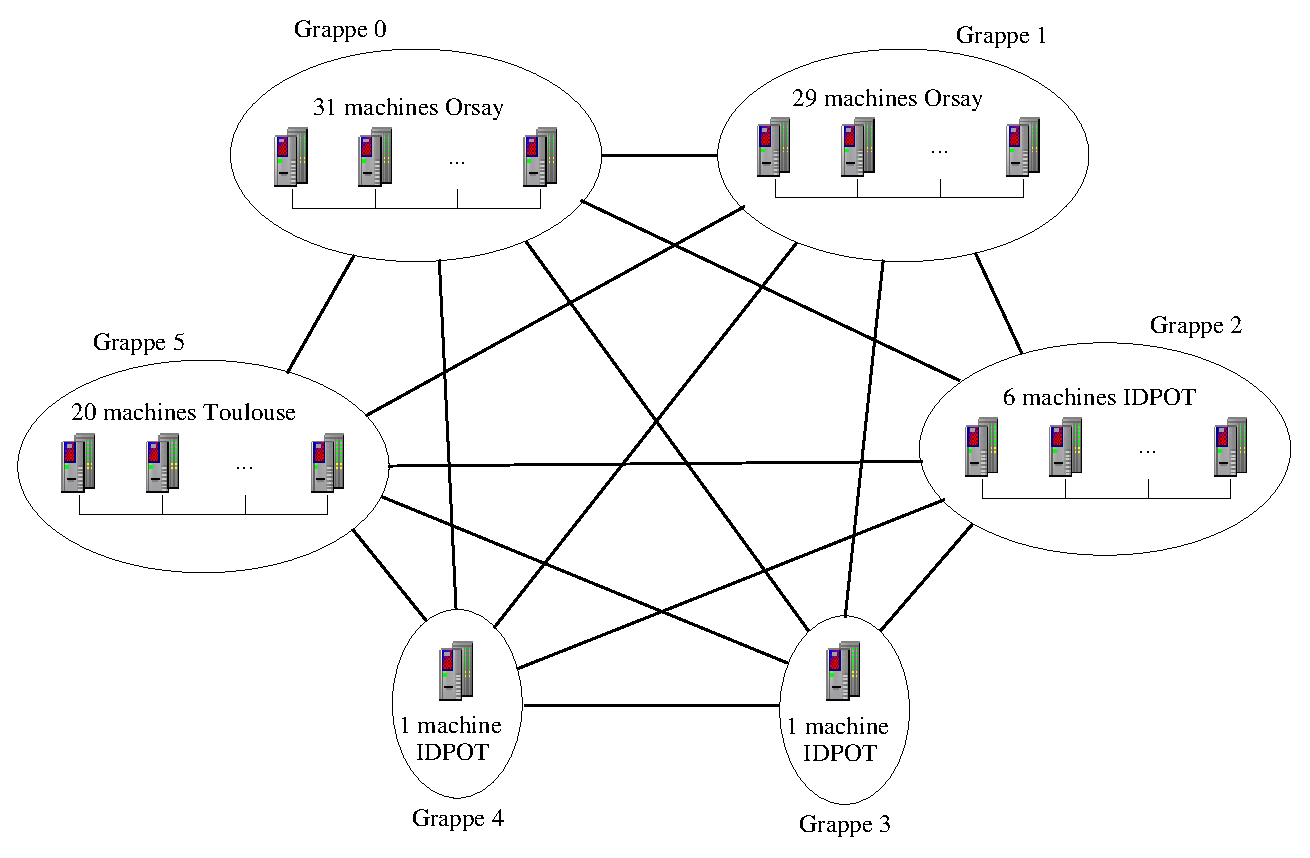
\includegraphics[width=0.75\linewidth]{images/Grid/Bcast/case1/grappe-case1}
%		\par\end{centering}
%	
%	\caption{\label{Figure: Bcast Grille 88 machines}Grille de 88 machines utilisée
%		dans les expérimentations pratiques}
%	
%\end{figure}
%

%Pour obtenir cette répartition des machines, on a utilisé l'algorithme
%de Lowekamp avec une tolérance de 30\%. Alors que le Tableau \ref{Tableau: Latence grid 1}
%indique la latence entre deux sites différents ou entre deux machines
%d'un même site (à part les grappes qui ont une seule machine), nous
%constatons des variations importantes de performance pour le réseau
%IDPOT. En effet, la latence d'interconnexion entre les machines IDPOT
%varie entre de $35\,\mu s$ et $242\,\mu s$, selon les machines.
%Ces variations sont dues surtout à l'utilisation de deux types différents
%de carte réseau, qui ont des performances distinctes, conformément
%à ce que nous avons indiqué dans \cite{Barchet04b}.

%
\begin{table}
	\caption{\label{Tableau: Latence grid 1}Latence entre les différents sites
		(en microsecondes)}
	
	
	\begin{centering}
		{\footnotesize }\begin{tabular}{|c||c|c|c|c|c|c|}
			\hline 
			& {\footnotesize Grappe 0} & {\footnotesize Grappe 1} & {\footnotesize Grappe 2} & {\footnotesize Grappe 3} & {\footnotesize Grappe 4} & {\footnotesize Grappe 5}\tabularnewline
			\hline 
			& {\footnotesize 31 x Orsay} & {\footnotesize 29 x Orsay} & {\footnotesize 6 x IDPOT} & {\footnotesize 1 x IDPOT} & {\footnotesize 1 x IDPOT} & {\footnotesize 20 x Toulouse}\tabularnewline
			\hline
			\hline 
			{\footnotesize Grappe 0} & {\footnotesize 47.56} & {\footnotesize 62.10} & {\footnotesize 12181.52} & {\footnotesize 12187.24} & {\footnotesize 12197.49} & {\footnotesize 5210.99}\tabularnewline
			\hline 
			{\footnotesize Grappe 1} & {\footnotesize 62.10} & {\footnotesize 47.92} & {\footnotesize 12181.52} & {\footnotesize 12198.03} & {\footnotesize 12195.22} & {\footnotesize 5211.47}\tabularnewline
			\hline 
			{\footnotesize Grappe 2} & {\footnotesize 12181.52} & {\footnotesize 12181.52} & {\footnotesize 35.52} & {\footnotesize 60.08} & {\footnotesize 60.08} & {\footnotesize 5388.49}\tabularnewline
			\hline 
			{\footnotesize Grappe 3} & {\footnotesize 12187.24} & {\footnotesize 12198.03} & {\footnotesize 60.08} & {\footnotesize 0$^{*}$} & {\footnotesize 242.47} & {\footnotesize 5393.98}\tabularnewline
			\hline 
			{\footnotesize Grappe 4} & {\footnotesize 12197.49} & {\footnotesize 12195.22} & {\footnotesize 60.08} & {\footnotesize 242.47} & {\footnotesize 0$^{*}$} & {\footnotesize 5394.10}\tabularnewline
			\hline 
			{\footnotesize Grappe 5} & {\footnotesize 5210.99} & {\footnotesize 5211.47} & {\footnotesize 5388.49} & {\footnotesize 5393.98} & {\footnotesize 5394.10} & {\footnotesize 27.53}\tabularnewline
			\hline
		\end{tabular}
		\par\end{centering}{\footnotesize \par}
	
	\begin{centering}
		{\footnotesize {*} cette grappe contient une seule machine.}
		\par\end{centering}
\end{table}


%Les mesures ont été effectuées en utilisant un processus de la grappe
%0 comme racine, et leur résultat est présenté dans la Figure \ref{Figure: Bcast - Case1 - Mesure}.
%On a comparé ces résultats avec l'implémentation \og pure \fg{} MPI,
%qui utilise des arbres binomiaux, comme décrit dans le chapitre \ref{cha:Mod=0000E9lisation des comms collectives}.
%Les prédictions de performance ont utilisé les valeurs de \emph{gap}
%et \emph{latence} (conformément au modèle pLogP) mesurées lors de
%l'initialisation de l'application, à travers la procédure de découverte
%de topologie décrite dans le chapitre \ref{cha: topo MPI}. Cependant,
%afin de permettre une meilleure compréhension de l'interconnexion
%entre les grappes, nous présentons les mesures des paramètres pLogP
%entre chaque grappe dans l'Annexe \ref{Annexe_A}.

Le premier résultat à noter est la faible performance de la stratégie
Flat, même par rapport à l'implémentation par défaut de LAM-MPI. Cela
ne veut pas dire que la stratégie Flat est toujours moins performante
que les autres stratégies, mais indique que cette stratégie est trop
dépendante de la configuration du réseau, de l'ordre de représentation
des grappes et du processus racine.

Dans le cas des autres heuristiques, on observe des gains de performance
déjà très importants. L'heuristique BottomUp %, comme prévu par lessimulations, 
n'est pas aussi efficace que les autres heuristiques,
qui de leur côté, se comportent de manière très similaire.

%
\begin{figure}[h]
	\begin{centering}
		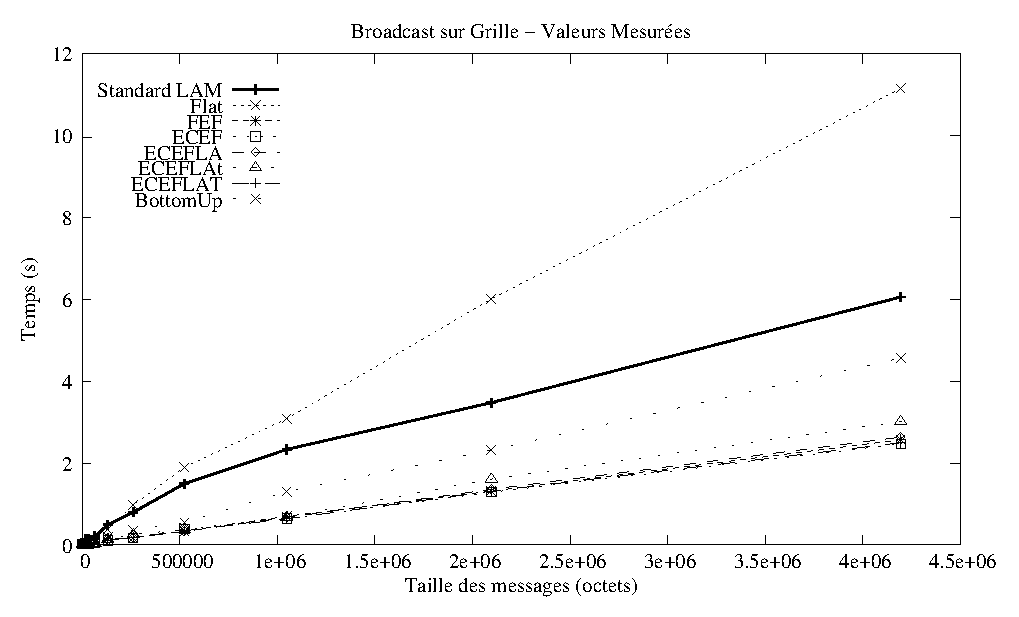
\includegraphics[width=0.8\linewidth]{images/Grid/Bcast/case1/comp}
		\par\end{centering}
	
	\caption{\label{Figure: Bcast - Case1 - Mesure}Performance du Broadcast sur
		une grille de 88 machines }
	
\end{figure}


Le faible écart observé entre les prédictions des heuristiques de
type FEF et ECEF-{*} est justifié surtout par le nombre réduit de
grappes, qui réduit le nombre de combinaisons possibles et fait converger
les résultats des différentes heuristiques. 

Pour mieux valider les résultats des expériences, la Figure \ref{Figure: Bcast case 1 predictions}
présente les temps prévus des différentes heuristiques. Ces temps,
calculés automatiquement par les heuristiques d'ordonnancement des
communications, donnent une meilleure indication de la fiabilité des
modèles par rapport aux résultats pratiques. Dans ce cas, nous observons
que les heuristiques de type FEF et ECEF-{*} ont des résultats très
rapprochés, certainement parce qu'elles ont obtenu le même ordonnancement
des communications. D'un autre côté, l'écart entre ces prédictions
et les résultats réels sont bien plus importants pour les heuristiques
FEF et ECEF-{*} que pour le BottomUp ou le Flat. Cela indique que
le coût du calcul de l'ordonnancement et le coût de la mise en oeuvre
de ces communications sont les facteurs les plus importants, et reflètent
l'augmentation de complexité d'une communication à couches multiples.

%
\begin{figure}[h]
	\begin{centering}
		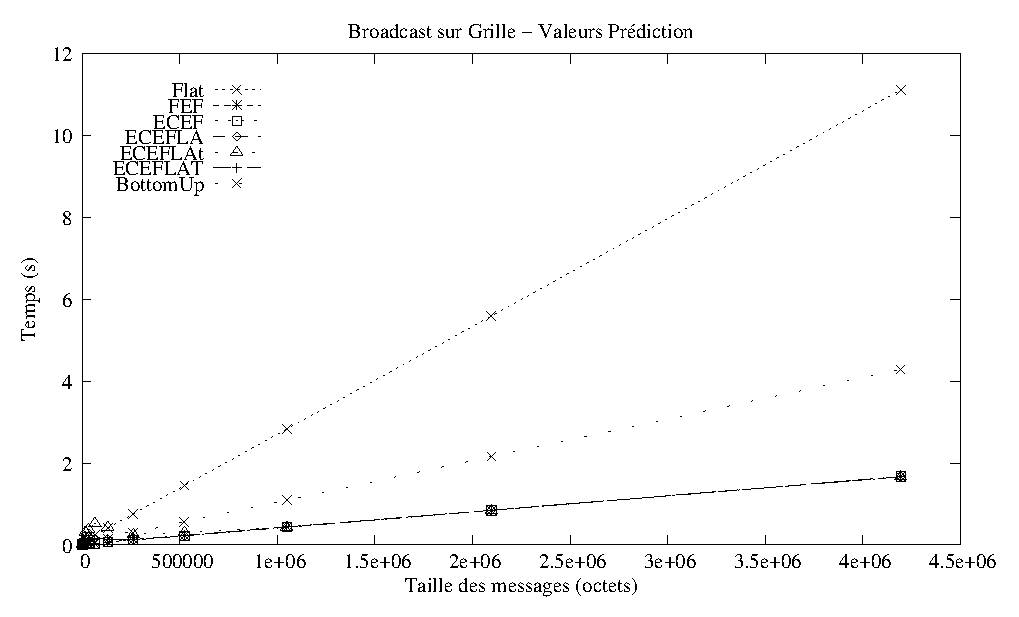
\includegraphics[width=0.8\linewidth]{images/Grid/Bcast/case1/simul}
		\par\end{centering}
	
	\caption{\label{Figure: Bcast case 1 predictions}Prédictions pour une grille
		avec 88 machines}
	
\end{figure}


%
%\subsubsection*{Cas No. 2}
%
%La deuxième expérience utilise 78 machines réparties entre les sites
%d'Orsay, Toulouse, Sophia-Antipolis et Grenoble (IDPOT). Alors que
%dans le cas précédent la majorité des machines appartenait à une seule
%grappe (Orsay), cette fois-ci nous avons utilisé des grappes plus
%équilibrées. En effet, nous avons utilisé 20 machines de la grappe
%GdX d'Orsay, 20 machines de la grappe de Toulouse, 19 machines de
%la grappe de Sophia-Antipolis et 17 machines de la grappe IDPOT.
%
%Comme dans le cas précédent, ces machines ont été regroupées en 6
%grappes homogènes différentes à l'aide de notre outil de découverte
%de topologie, qui implante l'algorithme de \emph{clustering} de Lowekamp.
%La disposition des grappes, représentée dans la Figure \ref{Figure: Bcast Grille 78 machines},
%est utilisée par la bibliothèque MagPIe pour établir la répartition
%des processus sur différentes grappes.
%
%%
%\begin{figure}[h]
%	\begin{centering}
%		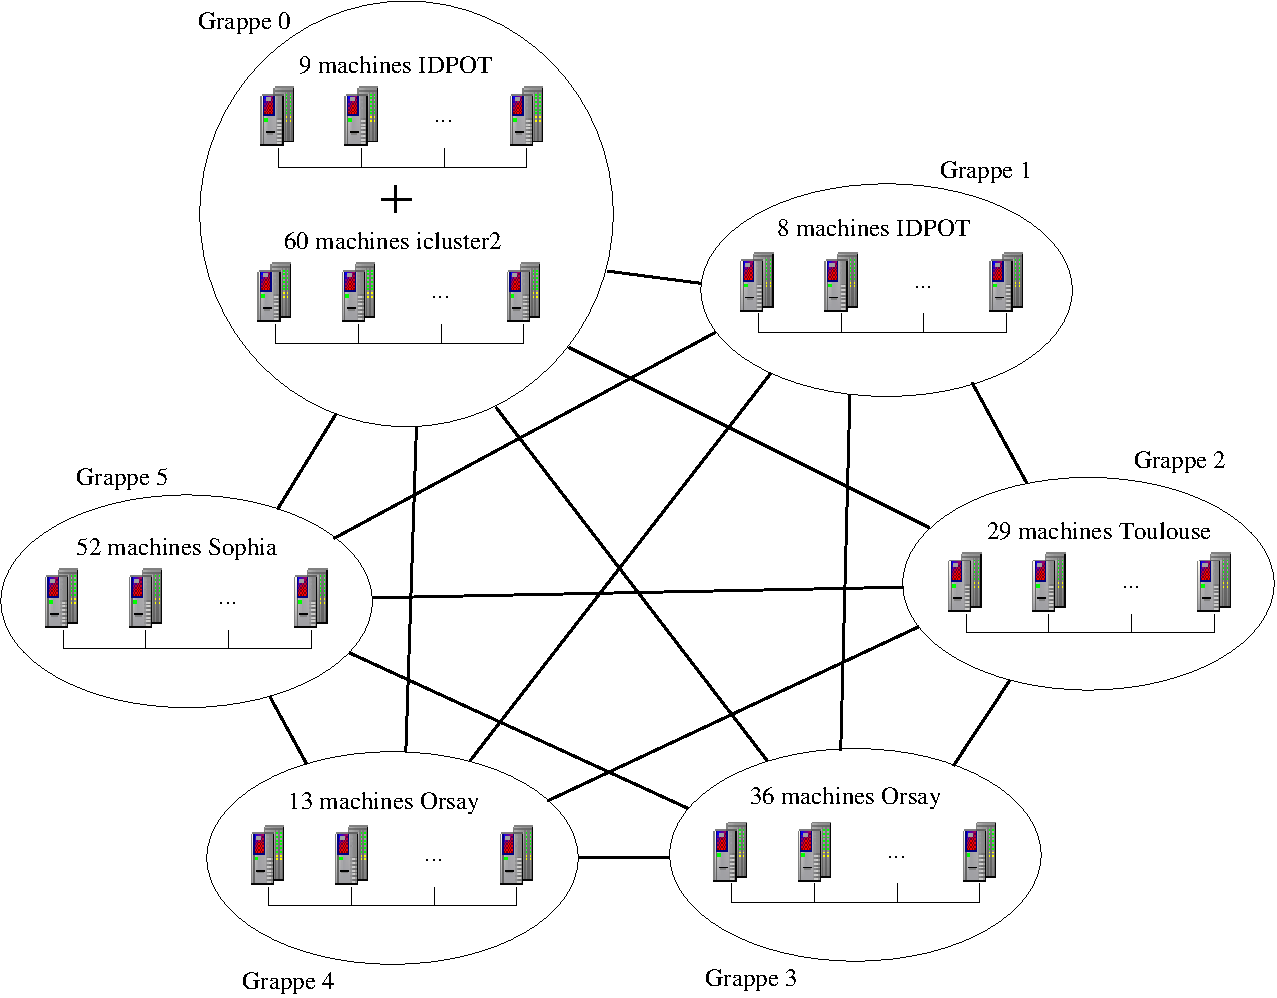
\includegraphics[width=0.75\linewidth]{images/Grid/Bcast/case2/grappe-case2}
%		\par\end{centering}
%	
%	\caption{\label{Figure: Bcast Grille 78 machines}Grille de 78 machines}
%	
%\end{figure}
%
%
%Les latences d'interconnexion entre les différents sites sont présentées
%dans le Tableau \ref{Tableau: bcast case 2 latences}. On observe
%que malgré la tolérance de 30\% utilisée par l'algorithme de \emph{clustering},
%la différence entre les machines IDPOT est suffisamment élevée pour
%forcer le regroupement des machines en plusieurs grappes.
%
%%
%\begin{table}
%	\caption{\label{Tableau: bcast case 2 latences}Latence entre les différents
%		sites (en microsecondes)}
%	
%	
%	\begin{centering}
%		{\footnotesize }\begin{tabular}{|c||c|c|c|c|c|c|}
%			\hline 
%			& {\footnotesize Grappe 0} & {\footnotesize Grappe 1} & {\footnotesize Grappe 2} & {\footnotesize Grappe 3} & {\footnotesize Grappe 4} & {\footnotesize Grappe 5}\tabularnewline
%			\hline 
%			& {\footnotesize 20 x Orsay} & {\footnotesize 11 x IDPOT} & {\footnotesize 7 x IDPOT} & {\footnotesize 1 x IDPOT} & {\footnotesize 20 x Toulouse} & {\footnotesize 19 x Sophia}\tabularnewline
%			\hline
%			\hline 
%			{\footnotesize Grappe 0} & {\footnotesize 48.39} & {\footnotesize 6577.49} & {\footnotesize 6586.49} & {\footnotesize 6592.51} & {\footnotesize 5211.94} & {\footnotesize 8602.73}\tabularnewline
%			\hline 
%			{\footnotesize Grappe 1} & {\footnotesize 6577.49} & {\footnotesize 35.52} & {\footnotesize 59.96} & {\footnotesize 59.96} & {\footnotesize 5387.48} & {\footnotesize 2736.56}\tabularnewline
%			\hline 
%			{\footnotesize Grappe 2} & {\footnotesize 6586.49} & {\footnotesize 59.96} & {\footnotesize 60.08} & {\footnotesize 79.51} & {\footnotesize 5393.98} & {\footnotesize 2740.26}\tabularnewline
%			\hline 
%			{\footnotesize Grappe 3} & {\footnotesize 6592.51} & {\footnotesize 59.96} & {\footnotesize 79.51} & {\footnotesize 0$^{*}$} & {\footnotesize 5405.78} & {\footnotesize 2745.98}\tabularnewline
%			\hline 
%			{\footnotesize Grappe 4} & {\footnotesize 5211.94} & {\footnotesize 5387.48} & {\footnotesize 5393.98} & {\footnotesize 5405.78} & {\footnotesize 26.94} & {\footnotesize 3630.51}\tabularnewline
%			\hline 
%			{\footnotesize Grappe 5} & {\footnotesize 8602.73} & {\footnotesize 2736.56} & {\footnotesize 2740.26} & {\footnotesize 2745.98} & {\footnotesize 3630.51} & {\footnotesize 35.04}\tabularnewline
%			\hline
%		\end{tabular}
%		\par\end{centering}{\footnotesize \par}
%	
%	\begin{centering}
%		{\footnotesize {*} cette grappe contient une seule machine.}
%		\par\end{centering}
%\end{table}
%
%
%Le résultat des mesures effectuées est présenté dans la Figure \ref{Figure: Bcast - case 2 - mesure}.
%On a comparé ces résultats avec l'implémentation \og pure \fg{} MPI,
%qui utilise des arbres binomiaux. Cette fois-ci, la disposition des
%grappes dans le fichier d'entrée de MagPIe a favorisé la stratégie
%Flat, qui a obtenu des performances similaires à celle des heuristiques
%plus élaborées. 
%
%%
%\begin{figure}[h]
%	\begin{centering}
%		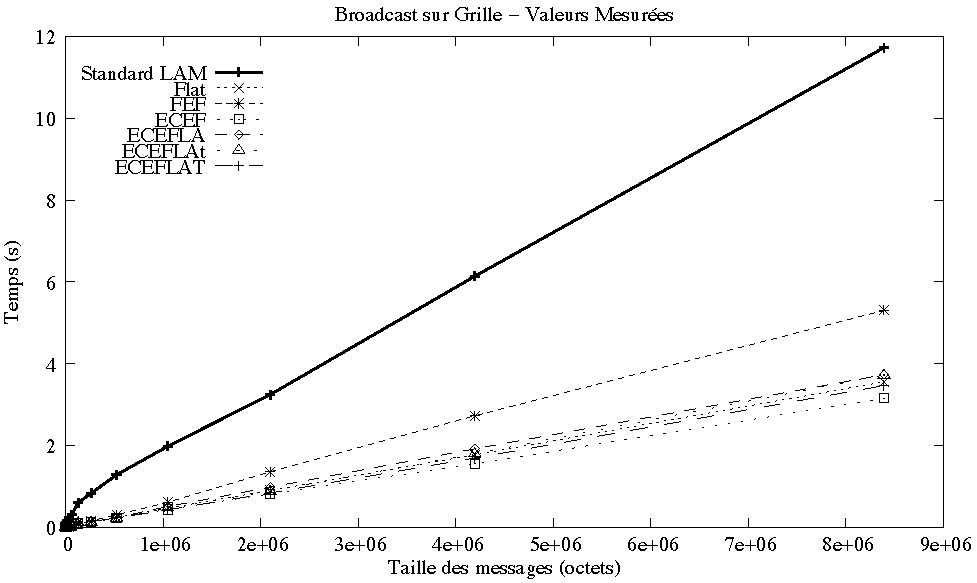
\includegraphics[width=0.8\linewidth]{images/Grid/Bcast/case3/comptipo3}
%		\par\end{centering}
%	
%	\caption{\label{Figure: Bcast - case 2 - mesure}Performance du Broadcast sur
%		une grille de 78 machines }
%	
%\end{figure}
%
%
%Dans un premier temps, l'analyse de la Figure \ref{Figure: Bcast - Case2 - zoom}
%indique que les heuristiques permettent un gain de performances important
%par rapport à l'algorithme en arbre binomial de la bibliothèque LAM-MPI.
%Parmi ces heuristiques, nous observons que les stratégies qui considèrent
%seulement la vitesse des liens, à l'instar de l'heuristique FEF, n'atteignent
%pas la meilleure performance. En effet, celle-ci est atteinte par
%les heuristiques de type ECEF, qui considèrent la disponibilité des
%processus, et non seulement la vitesse des liens. 
%
%Une remarque importante est que dans ce cas la stratégie Flat a obtenu
%des résultats similaires à ceux des meilleures heuristiques. Cela
%ne veut pas dire que l'heuristique Flat est optimale, mais seulement
%qu'elle est adaptée à l'ordre des grappes et au processus racine utilisé
%dans cette expérience. 
%
%%
%\begin{figure}[h]
%	\begin{centering}
%		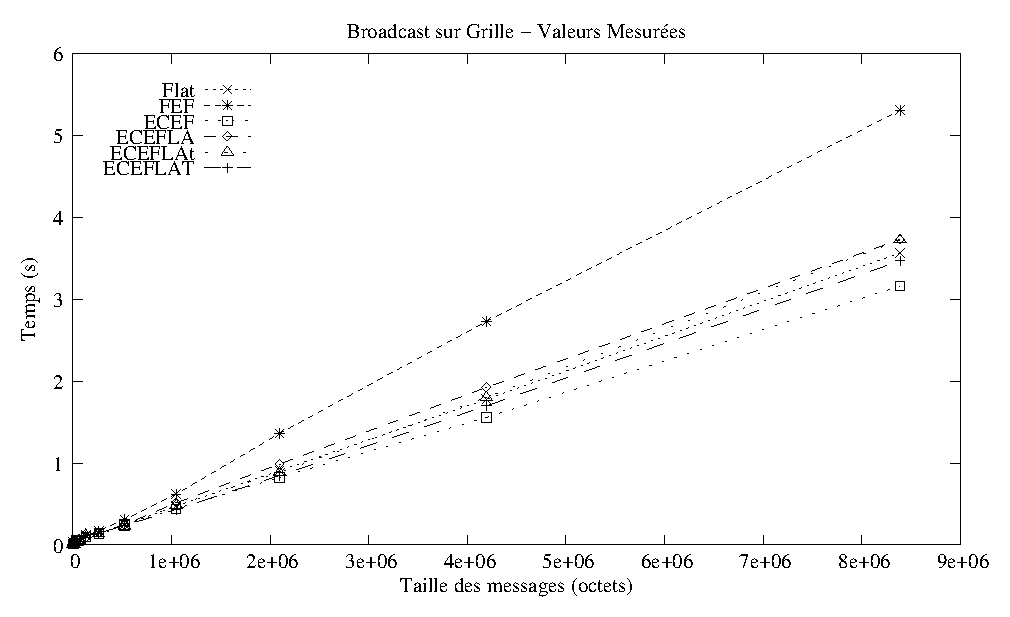
\includegraphics[width=0.8\linewidth]{images/Grid/Bcast/case3/comptipo3-zoom}
%		\par\end{centering}
%	
%	\caption{\label{Figure: Bcast - Case2 - zoom}Détails des performances des
%		heuristiques pour le Broadcast}
%	
%\end{figure}
%
%

\subsection{Considérations sur l'opération MPI\_Bcast }

Si dans un premier temps l'analyse des trois cas d'étude permet la
validation des certaines prédictions faites à travers la simulation
de différents environnements réseau, son apport le plus important
est l'observation du comportement des implémentations des heuristiques. 

Les trois situations étudiées ont notamment mis en évidence l'importance
du processus racine et de la répartition des processus sur des différentes
grappes sur la performance des stratégies plus simples. En effet,
la performance de la stratégie Flat est fortement liée à l'ordre de
représentation des grappes répartition, généralement fournie par l'utilisateur.
De surcroît, la stratégie Flat utilise toujours le même ordre de diffusion,
indépendamment du rang du processus racine. Au contraire, les heuristiques
les plus élaborées construisent des arbres de diffusion adaptés à
chaque situation, ce qui rend possible un gain de performance plus
important, surtout quand le rôle de \emph{racine} est alterné entre
plusieurs processus.

D'ailleurs, les simulations indiquent que la performance des stratégies
simples, comme le Flat, supportent très mal l'augmentation du nombre
de grappes interconnectées. Ceci met en cause l'efficacité de ces
stratégies dans un futur proche. Ainsi, nous croyons que, même si
la grille compte un nombre réduit de grappes, l'utilisation d'une
heuristique un peu plus élaborée, comme par exemple l'heuristique
ECEFLA-T, offre le meilleur rapport coût-bénéfice-robustesse.




\section{Bilan et Perspectives}

Dans ce chapitre nous avons présenté une stratégie efficace pour identifier
et découper les réseaux en grappes logiques homogènes. La présence
des hétérogénéités réduit la précision des modèles de communication
utilisés pour optimiser les communications collectives. Le \emph{framework}
proposé réussi à obtenir des paramètres de connectivité par un coût
très faible, à partir du regroupement d'informations obtenues indépendamment
dans chaque grappe. Notre approche, validée par des tests pratiques,
démontre que la découverte de topologie peut se faire de façon rapide
et précise. Associé à des modèles de prédiction de performance, le
découpage des grappes s'avère essentiel à l'optimisation des primitives
de communication collective, spécialement pour celles structurées
en multiples couches. De plus, ce \emph{framework} peut être étendu,
de manière à détecter aussi la présence de machines multiprocesseur,
information importante pour l'optimisation des communications.

Toutefois, la découverte de topologie a aussi des applications avec
d'autres domaines que le calcul parallèle. En effet, nous avons travaillé
au début de cette thèse avec l'application de la topologie sur les
algorithmes repartis comme la Diffusion Totalement Ordonnée. Ainsi,
l'Annexe \ref{cha:topo FT} montre comme la connaissance de la topologie
du réseau peut être utilisée pour augmenter la performance des algorithmes
repartis, réputés peu performants.


